\subsection{Results}
\label{Results3}
\setlength{\parindent}{20pt}
\justifying

\subsubsection{\large{\emph{Participants}}}
\label{Exp3_ParticipantExclusion}

\noindent
Two hundred participants were recruited for the third experiment. Four participants were then found to have average response times during testing over 2 seconds, which led to their exclusion. One participant responded ``yes'' to all items presented in the testing phase, and was also excluded. This left 195 participants' data in the final analysis sample. These were made up of 138 males, and participants' mean age was 22.21 years.



\subsubsection{\large{\emph{Group-level analyses}}}

\noindent
\underline{Familiarity test}

\noindent 
Despite the removal of the morpheme spelling task, familiarity scores rose considerably (t(194) = 17.91, p $<$ 2.2e$^{-16}$, estimate = 66\%). This represents a 9\% increase from experiment 2. The mean response time was also approximately 150 ms quicker in this version, at 1515 ms on average. This increase in accuracy combined with a decrease in response times provides evidence that participants segmented the words more easily than previously.

\begin{figure}[!htbp]
    \begin{center}
        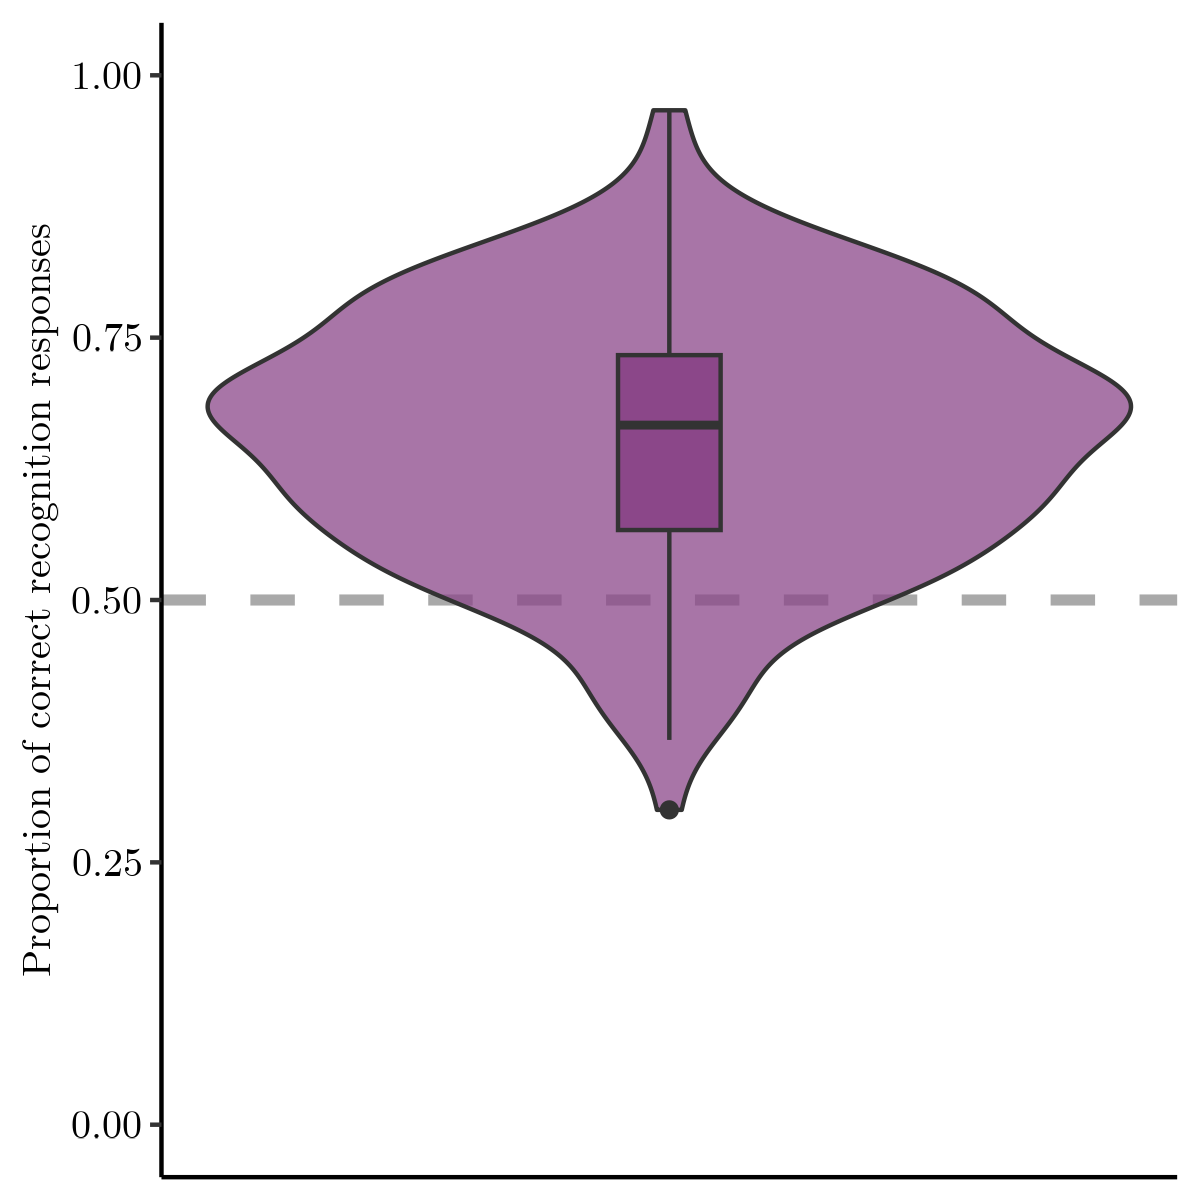
\includegraphics[width=0.6\textwidth]{Figures/exp3_familiarity_violinplt.png}
    \end{center}
    \caption[]{\justifying Violin plot and boxplot of the accuracy of familiarity test responses. The dashed line indicates chance level.}
    \label{exp3_familiarity}
\end{figure}

\noindent
\underline{Morpheme familiarity effect}

\noindent
In line with both previous experiments, the morpheme familiarity effect was strong also in experiment 3. Linear modelling found significant differences in responses between the 0M (Intercept, $\beta$ = -0.50, z-value = -10.96, p = 6.2e$^{-28}$), 1M ($\beta$ = 0.63, z-value = 18.16, p = 1.0e$^{-73}$), and 2M ($\beta$ = 1.25, z-value = 35.22, p = 1.0e$^{-271}$) conditions. Estimated marginal means revealed that participants tended to reject items from the 0M condition (model fit of the proportion of ``yes'' responses = 0.38, SE = 0.01), responded near but above chance level for 1M items (model fit = 0.53, SE = 0.01), and strongly preferred 2M items (model fit = 0.68, SE = 0.01). This is a pattern of responses more balanced around chance level: while in experiment 2, responses to the 0M condition where those around chance level, participants in this design were more able to respond ``no'' to 0M items, and we see instead the cluster of 1M responses fall around chance. This might indicate some hesitation for participants: it seems clearer to reject items with no familiar morphemes here, but those with one familiar word part tied to an unfamiliar string elicit some confusion as to whether to accept these. 

\begin{figure}[!htbp]
    \begin{center}
        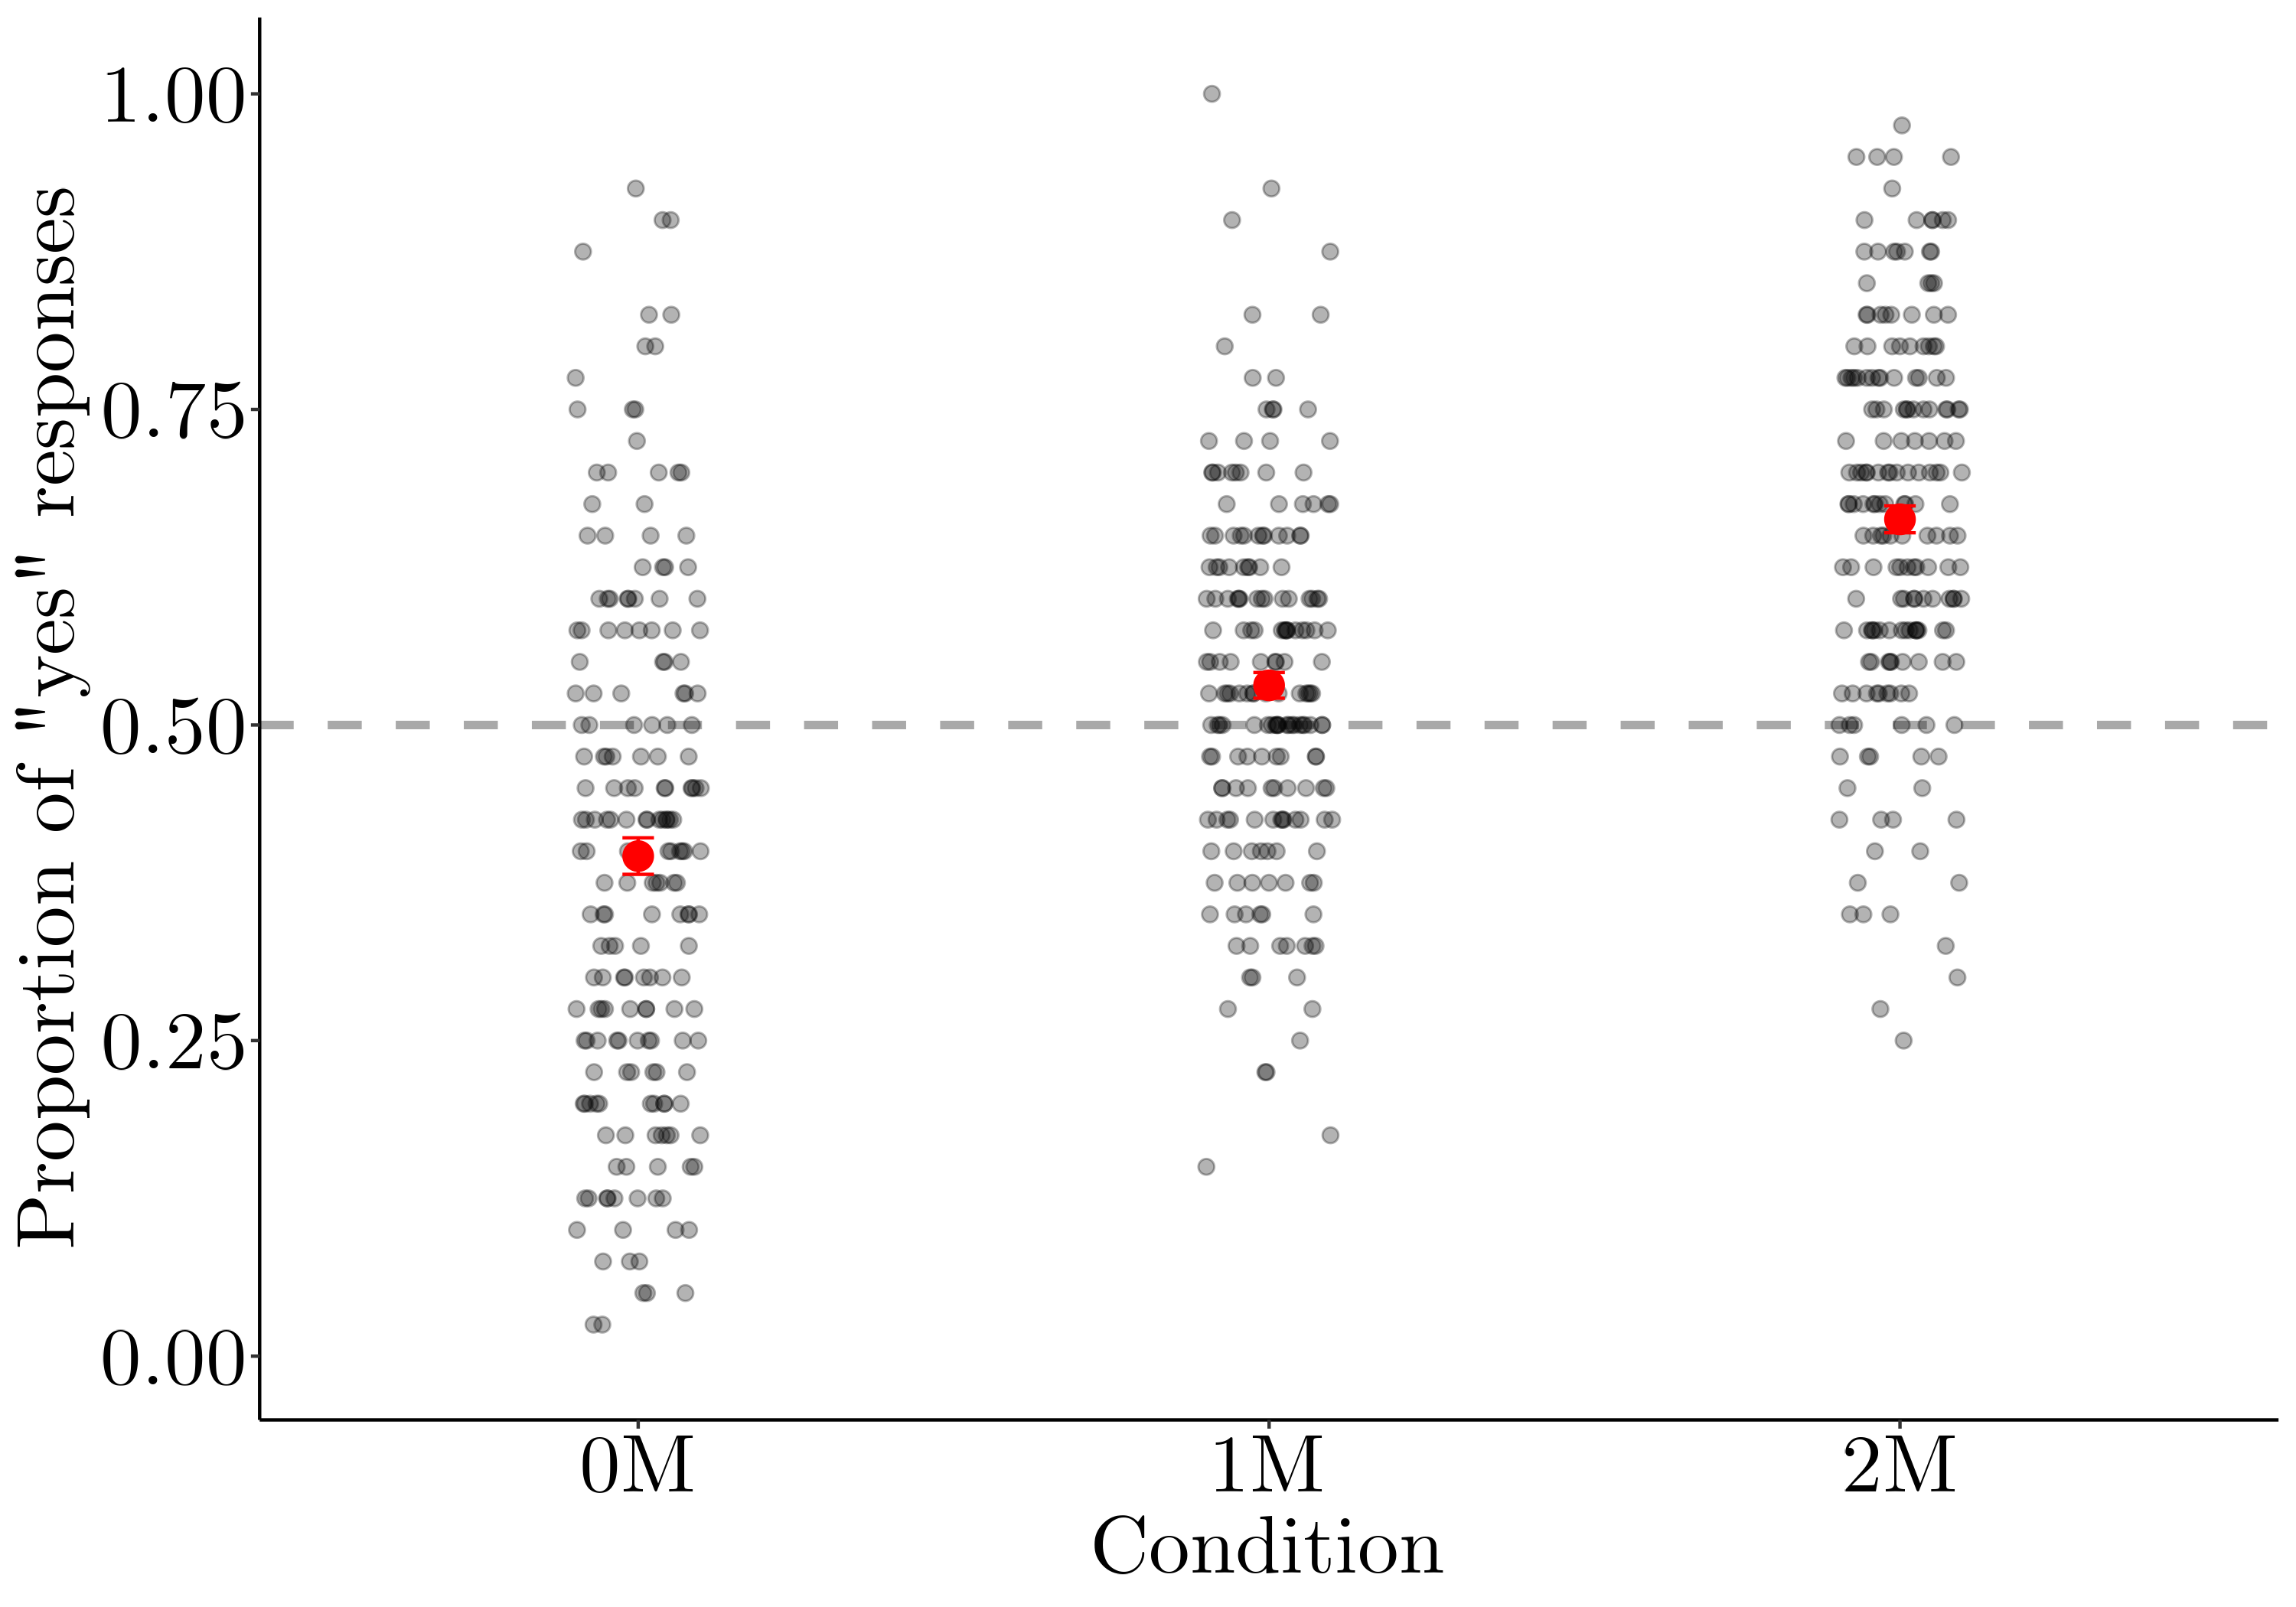
\includegraphics[width=0.6\textwidth]{Figures/exp3_yes_allconditions_scatterplot.png}
    \end{center}
    \caption[]{\justifying Proportion of ``yes'' responses in each testing condition. The dashed line indicates chance level. The red circle shows the group mean, with bars as the standard error of the mean.}
    \label{exp3_morphfam}
\end{figure}


\noindent
\underline{2M performance}

\noindent
As for performance in the 2M condition, participants were able to distinguish between within- and between-language combinations (t(194) = 2.68, p = 0.008, estimate = 0.51). The mean d-prime of participants was 0.07 (t(194) = 2.61, p = 0.01), indicating further that the underlying pattern was detected. The mean c value was of -0.44 (t(194) = -14.40, p $<$ 2.2e$^{-16}$). This is a slightly stronger ``yes'' bias than in previous versions, but with responses more in tune with stimulus nature.


\begin{figure}[!htbp]
    \begin{center}
        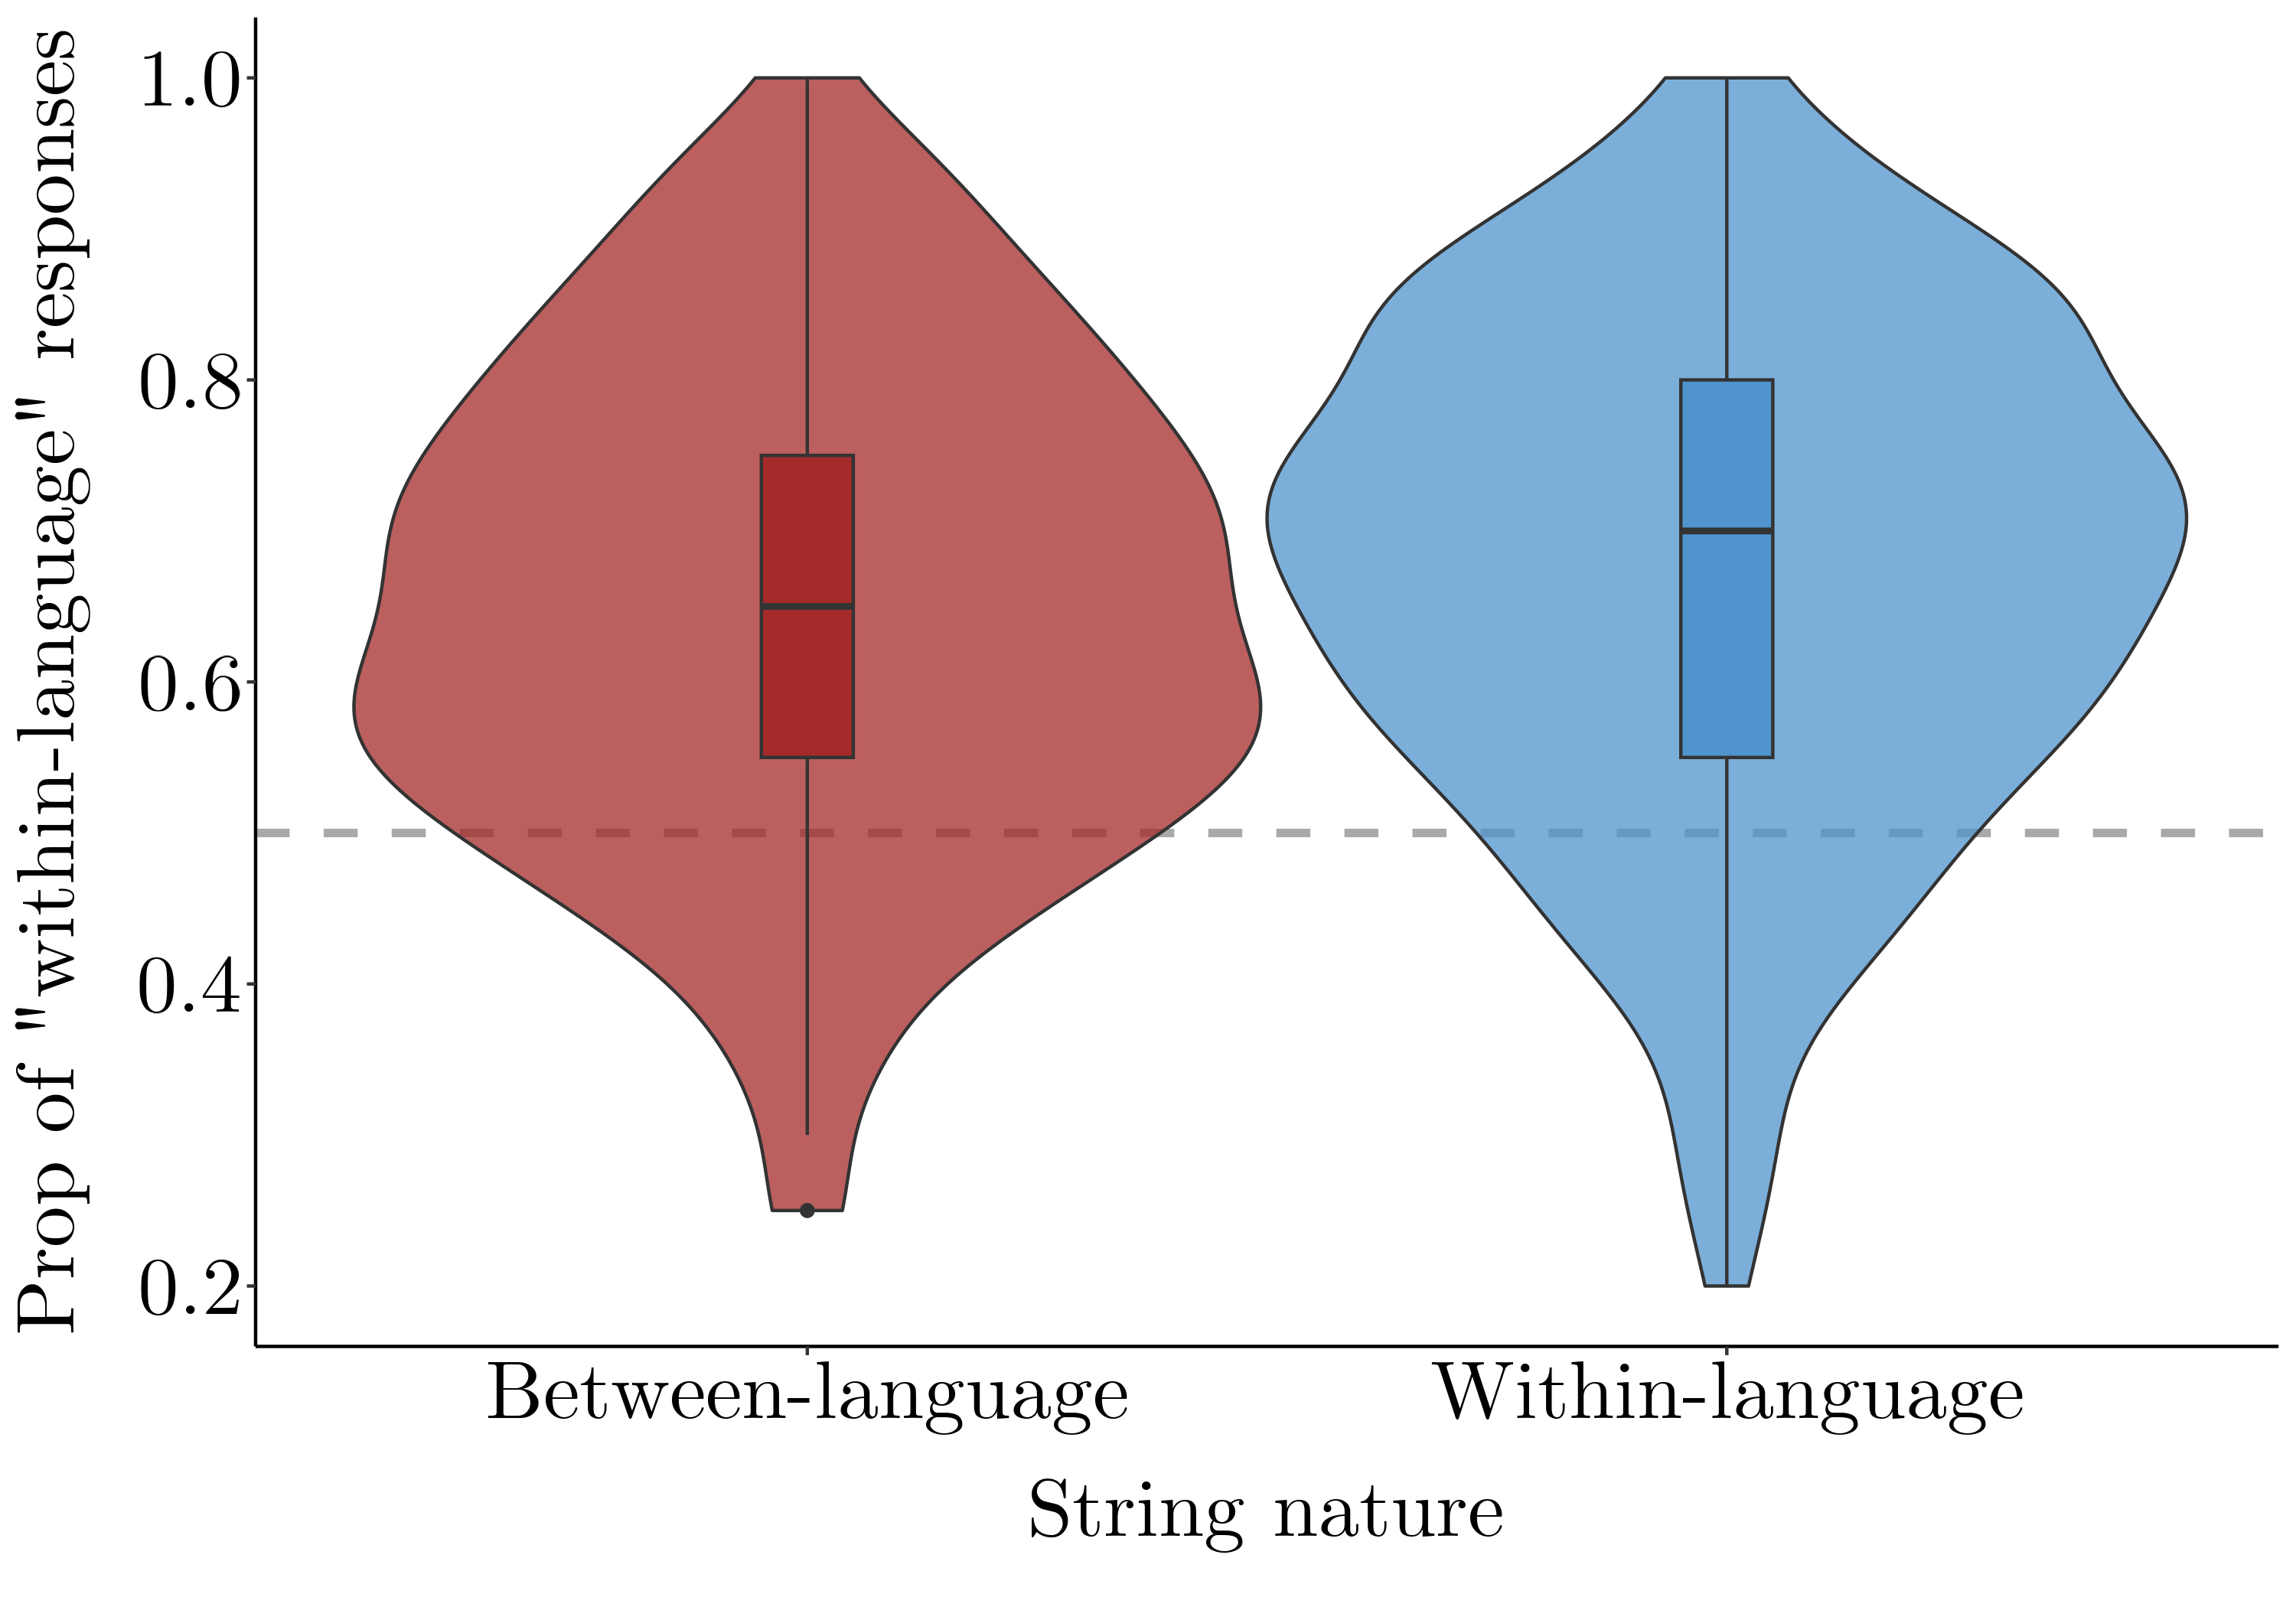
\includegraphics[width=0.6\textwidth]{Figures/exp3_2M_responses.png}
    \end{center}
    \caption[]{\justifying Boxplots of the proportion of ``within-language'' responses to each 2M combination type. The dashed line indicates chance level.}
    \label{exp3_2Mresponses}
\end{figure}


\subsubsection{\large{\emph{Individual differences analyses}}}

\noindent
\underline{BLP}

\noindent
Analysis of the Bilingual Language Profile showed 23 participants only speaking one language, 91 speaking two, 55 speaking three, and 26 speaking four. The most common L1 was Arabic, English the most common L2, and French the most common L3 and L4. Of the declared languages, these belonged to 6 different language families, and represented 13 different language branches. This sample therefore had 105 participants who used languages with one same script, and 90 who used languages with different scripts.

\noindent
\underline{PCA}

\noindent
The Principal Components Analysis on experiment 3's BLP data revealed four components of interest. PC1 loaded L4 history, use, proficiency, and attitudes, and accounted for 21\% of variance in the data. PC3 was the equivalent for L3 metrics, explaining 20\% of variance. PC2, like in experiments 1 and 2, looked at the balance between L1 and L2 language use. This was responsible for 10\% of variance. Finally, PC8, also present in experiments 1 and 2, included L2 history information, and held 6\% of variance.


\noindent
\underline{Familiarity test}

\noindent
In this version of the experiment, none of our measures significantly predicted familiarity responses. It is possible that stimulus parameters (namely, their presentation in a familiar script) made segmentation so straightforward as to not require the aid or involvement of other linguistic capabilities.

\noindent
\underline{Morpheme familiarity effect}

\noindent
Overall, participants who had more balanced multilingual profiles (as computed by cosine similarity) tended to respond with a stronger ``yes'' bias than other participants (cosine similarity main effect $\beta$ = 3.33, z = 2.52, p = 0.01).

\begin{figure}[!htbp]
    \begin{center}
        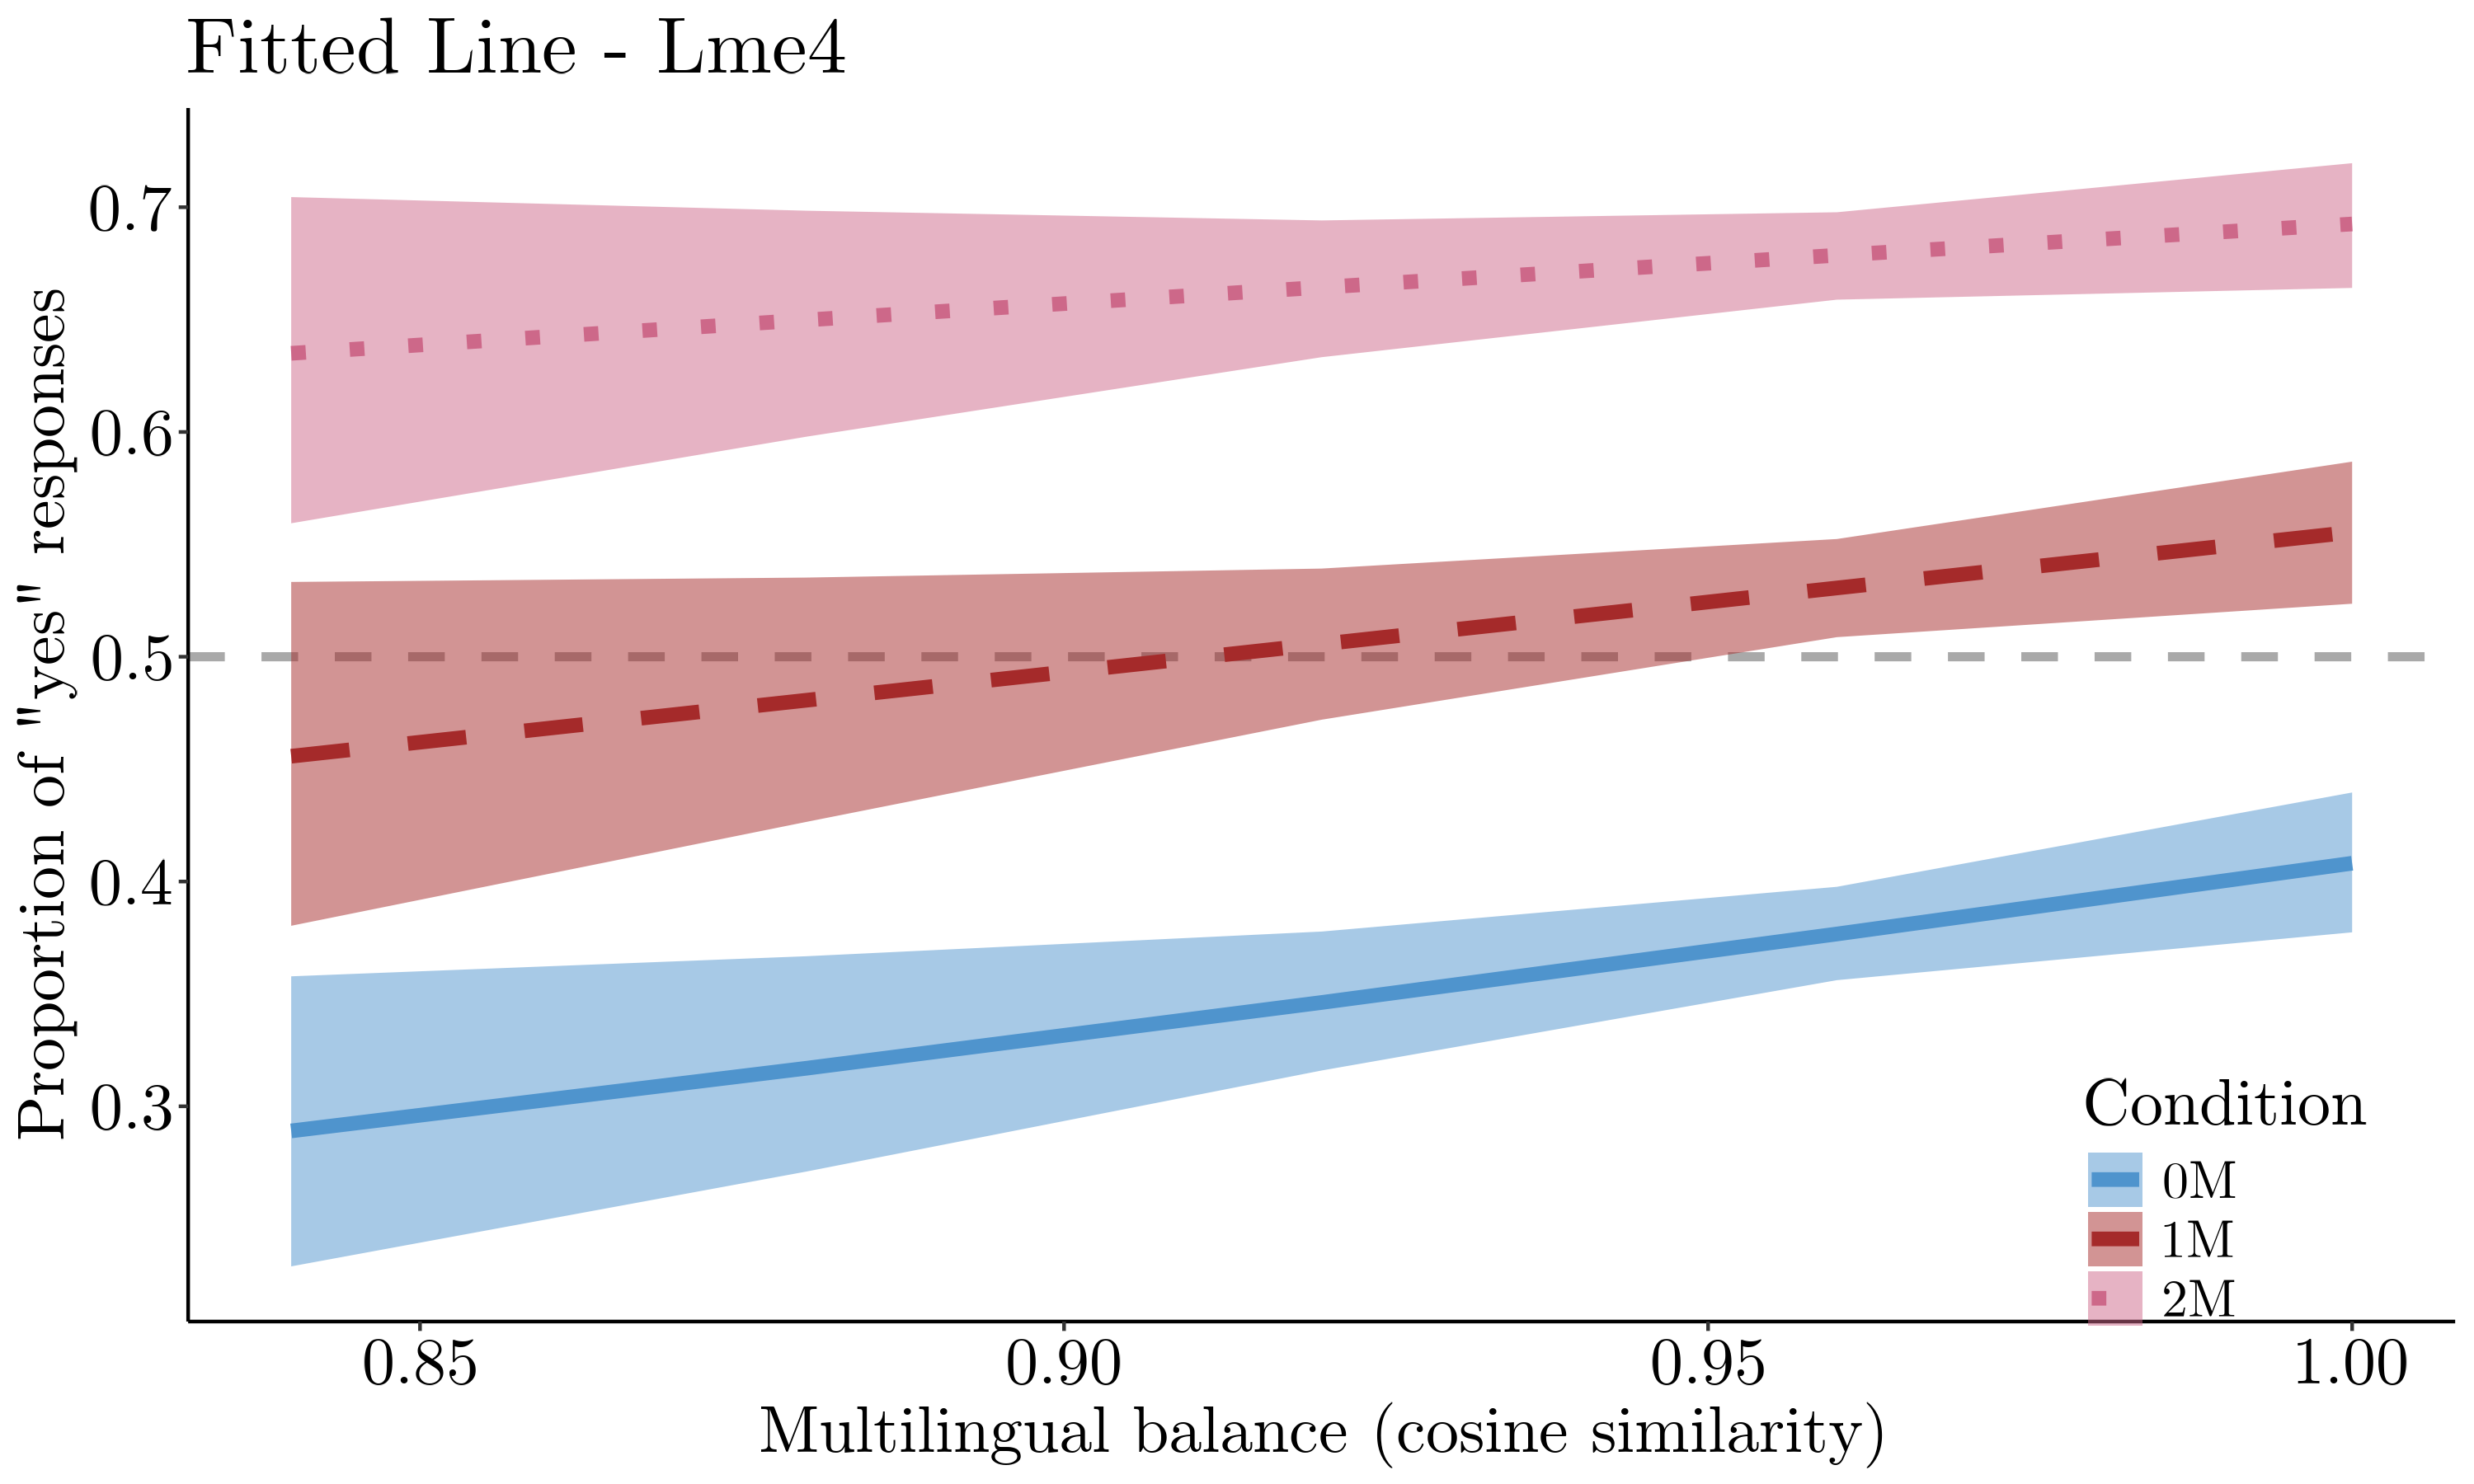
\includegraphics[width=0.6\textwidth]{Figures/exp3_yes_cossim.png}
    \end{center}
    \caption[]{\justifying Model estimates of the effect of the amount of ``yes'' responses over all testing conditions, in relation to multilingual balance (cosine similarity). Cosine similarity scores closer to 1 indicate more balance across a participants' languages. Shaded areas around the lines indicate the 95\% confidence interval. The dashed line at 50\% indicates chance level.}
    \label{exp3_yes_cossim}
\end{figure}

As in experiment 2, participant gender influenced propensity to respond ``yes'' to known morphemes, with women showing not only a lesser proportion of ``yes'' responses over all items (Women main effect $\beta$ = -0.25, z = -2.45, p = 0.01), but also different responses across stimuli than men (1M*Women interaction $\beta$ = 0.15, z = 1.98, p = 0.048; 2M*Women interaction $\beta$ = 0.18, z = 2.29, p = 0.02). 

Multiple multilingual metrics also affected ``yes'' responses. PC1, loading L4 information, revealed accentuated differences between the different testing conditions when participants had low L4 scores (2M*PC1 interaction $\beta$ = -0.11, z = -3.04, p = 0.002). Another PC component, PC2, showed an effect of increase second-language: the more participants made use of their L2 rather than their L1, the stronger their morpheme familiarity effect was (1M*PC2 interaction $\beta$ = 0.10, z = 2.88, p = 0.004; 2M*PC2 interaction $\beta$ = 0.19, z = 5.24, p = 1.61e$^{-7}$). Higher levels of multilingual balance (entropy) also exaggerate the morpheme familiarity effect (1M*entropy interaction $\beta$ = 0.18, z = 2.70, p = 0.01; 2M*entropy interaction $\beta$ = 0.28, z = 4.02, p = 5.20e$^{-5}$).

\begin{figure}[!htbp]
    \begin{minipage}{0.49\linewidth}
        \includegraphics[width=0.99\textwidth]{Figures/exp3_yes_Gender.png}
    \end{minipage}
    \begin{minipage}{0.49\linewidth}
        \centering
        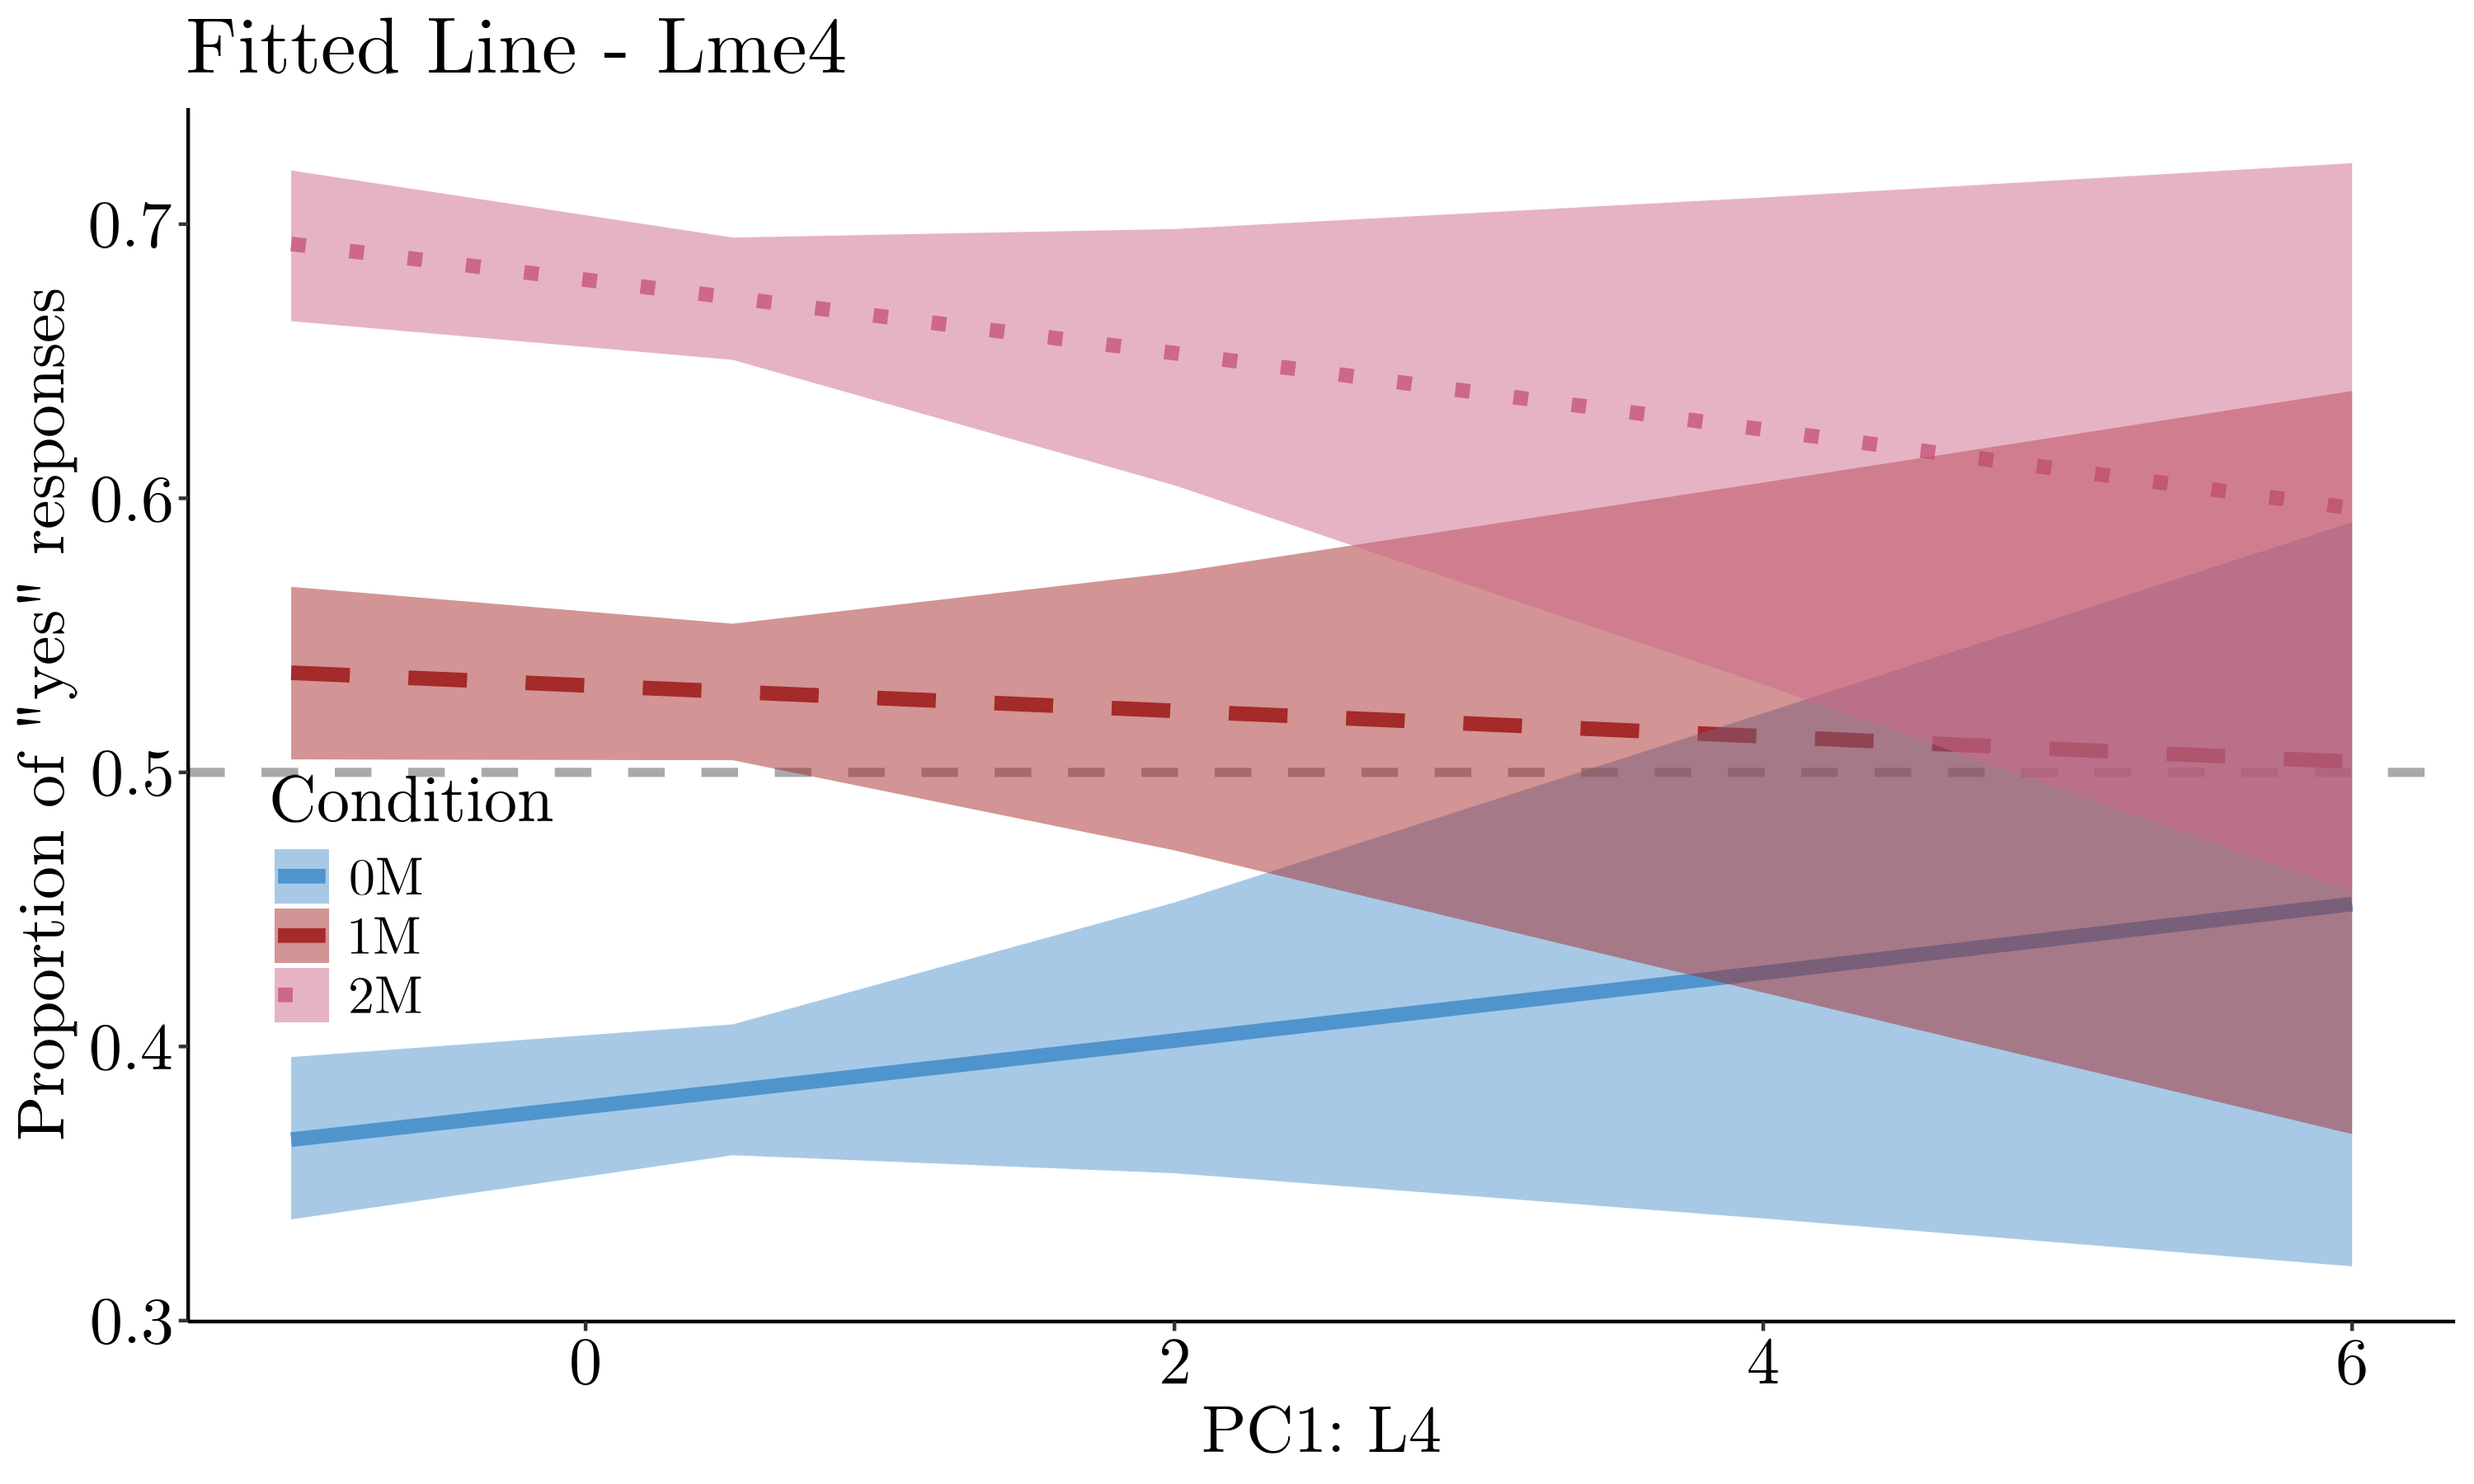
\includegraphics[width=0.99\textwidth]{Figures/exp3_yes_RC1.png}
    \end{minipage}
    \begin{minipage}{0.49\linewidth}
        \centering
        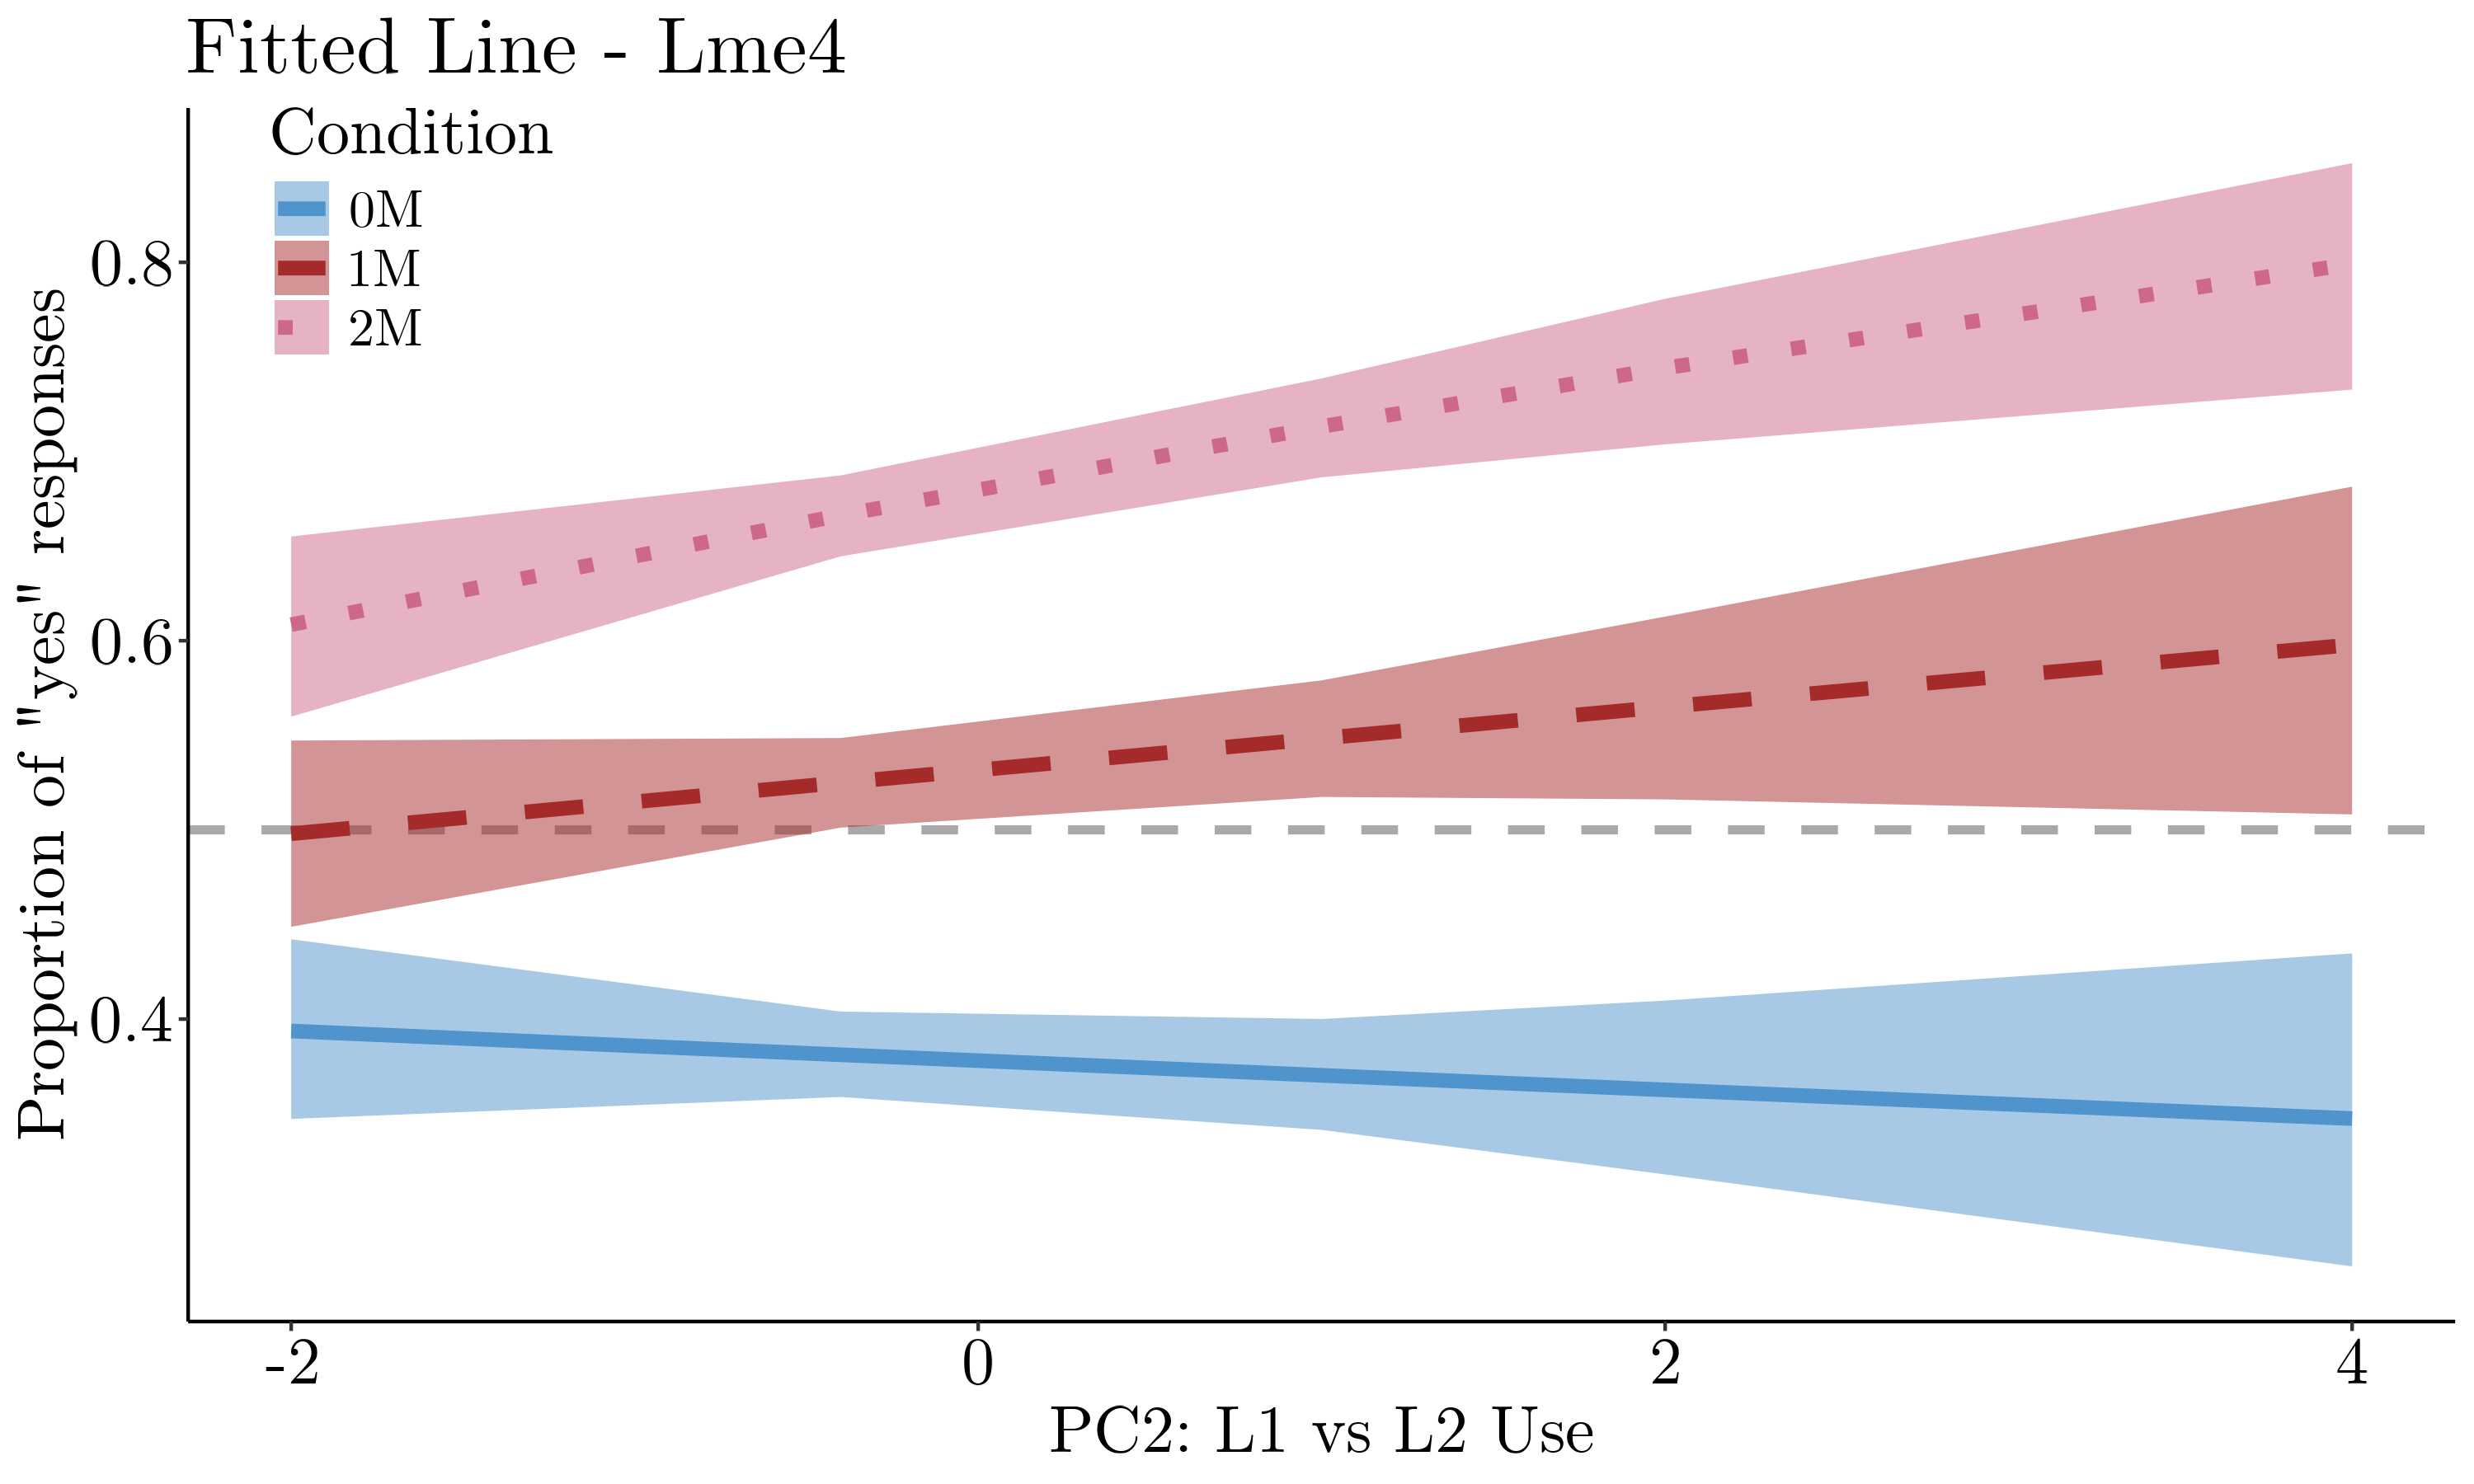
\includegraphics[width=0.99\textwidth]{Figures/exp3_yes_RC2.png}
    \end{minipage}
    \begin{minipage}{0.49\linewidth}
        \centering
        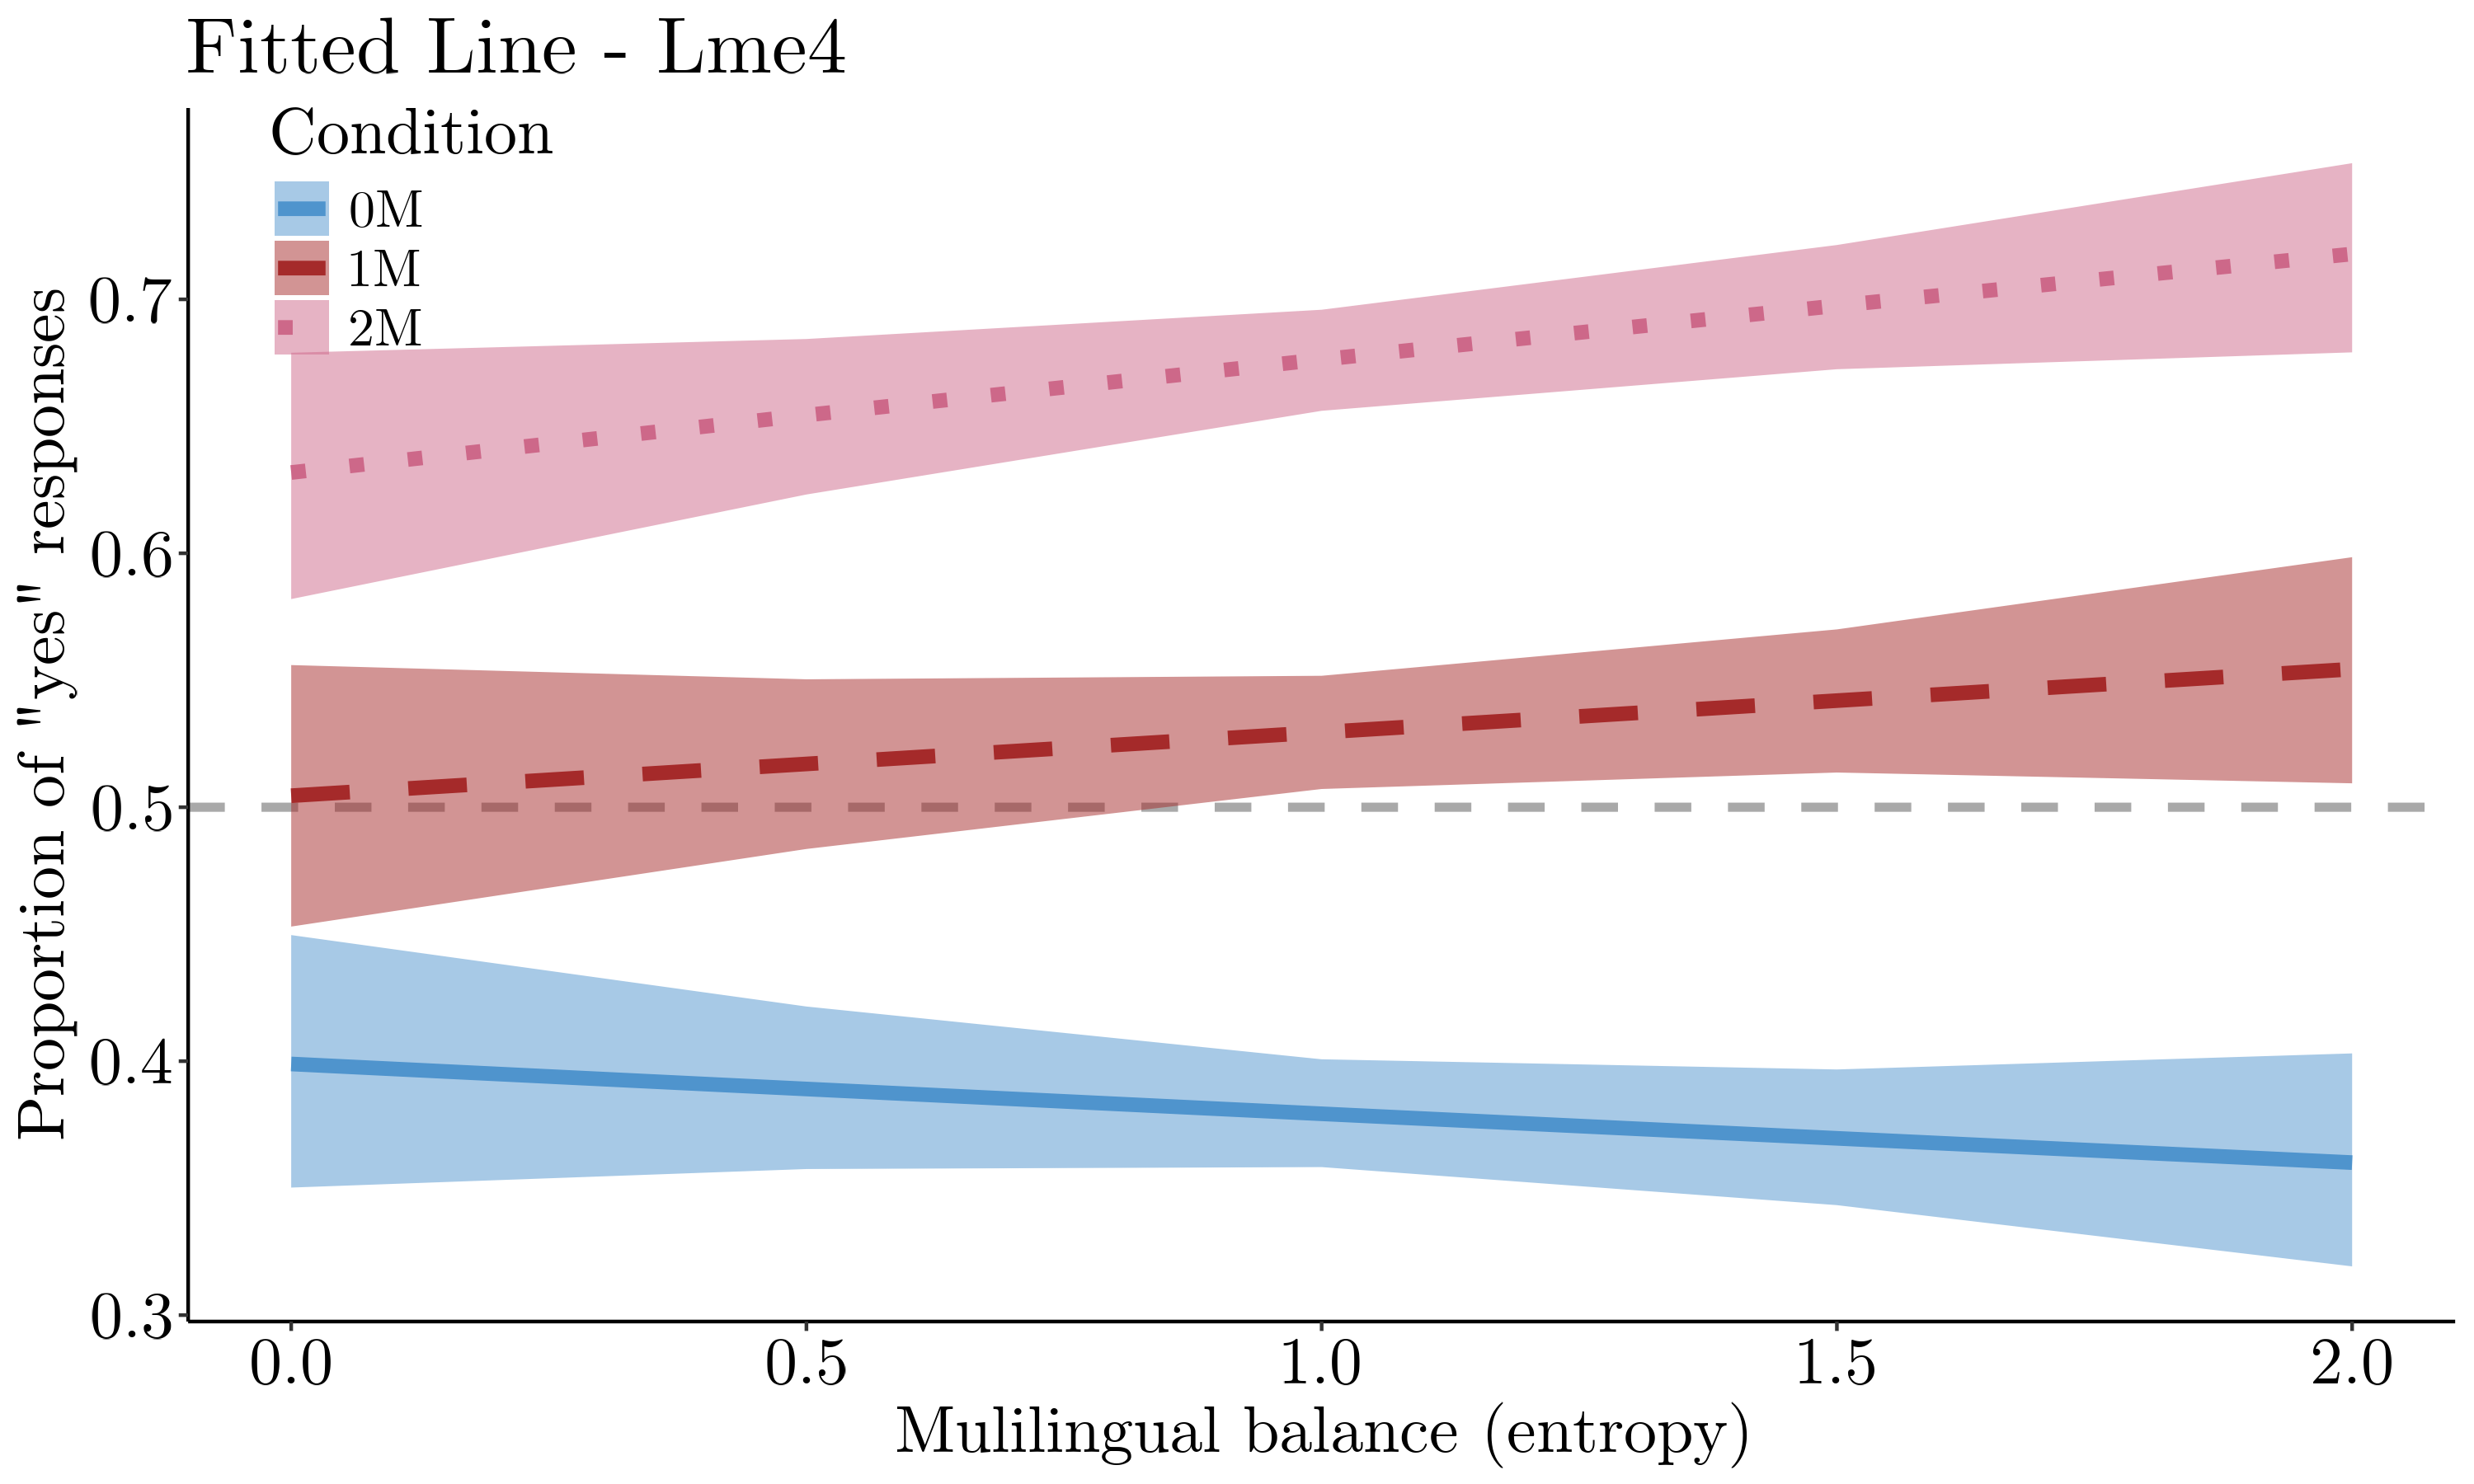
\includegraphics[width=0.99\textwidth]{Figures/exp3_yes_ent.png}
    \end{minipage}
    \caption[]{\justifying Model estimates of the effect of gender (top left), PC1 (L4; top right), PC2 (L1 vs L2 use; bottom left), and multilingual balance (entropy; bottom right)  on ``yes'' responses, for the 0M (blue; solid), 1M (red; dashed), and 2M (pink; dotted)conditions. Higher levels of PC2 means more L2 rather than L1 use. Higher levels of entropy mean a more balanced multilingual profile. Shaded areas around the lines indicate the 95\% confidence interval. The black dashed line at 0.5 indicates chance level.}
    \label{exp3_yes_gender/PC1/PC2/ent}
\end{figure}

Further metrics also interacted with the different testing conditions. Participants with more multilingual experience were more sensitive to the presence of familiar morphemes in testing input (2M*multilingual experience interaction $\beta$ = 0.10, z = 2.71, p = 0.007). Increased balance between participants' first languages also boosted morpheme sensitivity (1M*L1-L2 difference interaction $\beta$ = -0.10, z = -2.77, p = 0.006; 2M*L1-L2 difference interaction $\beta$ = -0.15, z = -4.19, p = 2.85e$^{-5}$). There also seems to be a different pattern of morpheme awareness depending on the number of languages that participants declared to speak. Bilinguals (2M*bilinguals interaction $\beta$ = 0.24, z = 2.07, p = 0.04) and trilinguals (1M*trilinguals interaction $\beta$ = 0.36, z = 2.07, p = 0.04; 2M*trilinguals interaction $\beta$ = 0.54, z = 4.38, p = 1.17e$^{-5}$) both have a stronger morpheme familiarity effect than monolinguals. Quadrilinguals, on the other hand, have different amounts of ``yes'' responses only for the 2M condition (2M*quadrilinguals interaction $\beta$ = 0.32, z = 2.25, p = 0.02).

\begin{figure}[!htbp]
    \begin{minipage}{0.49\linewidth}
        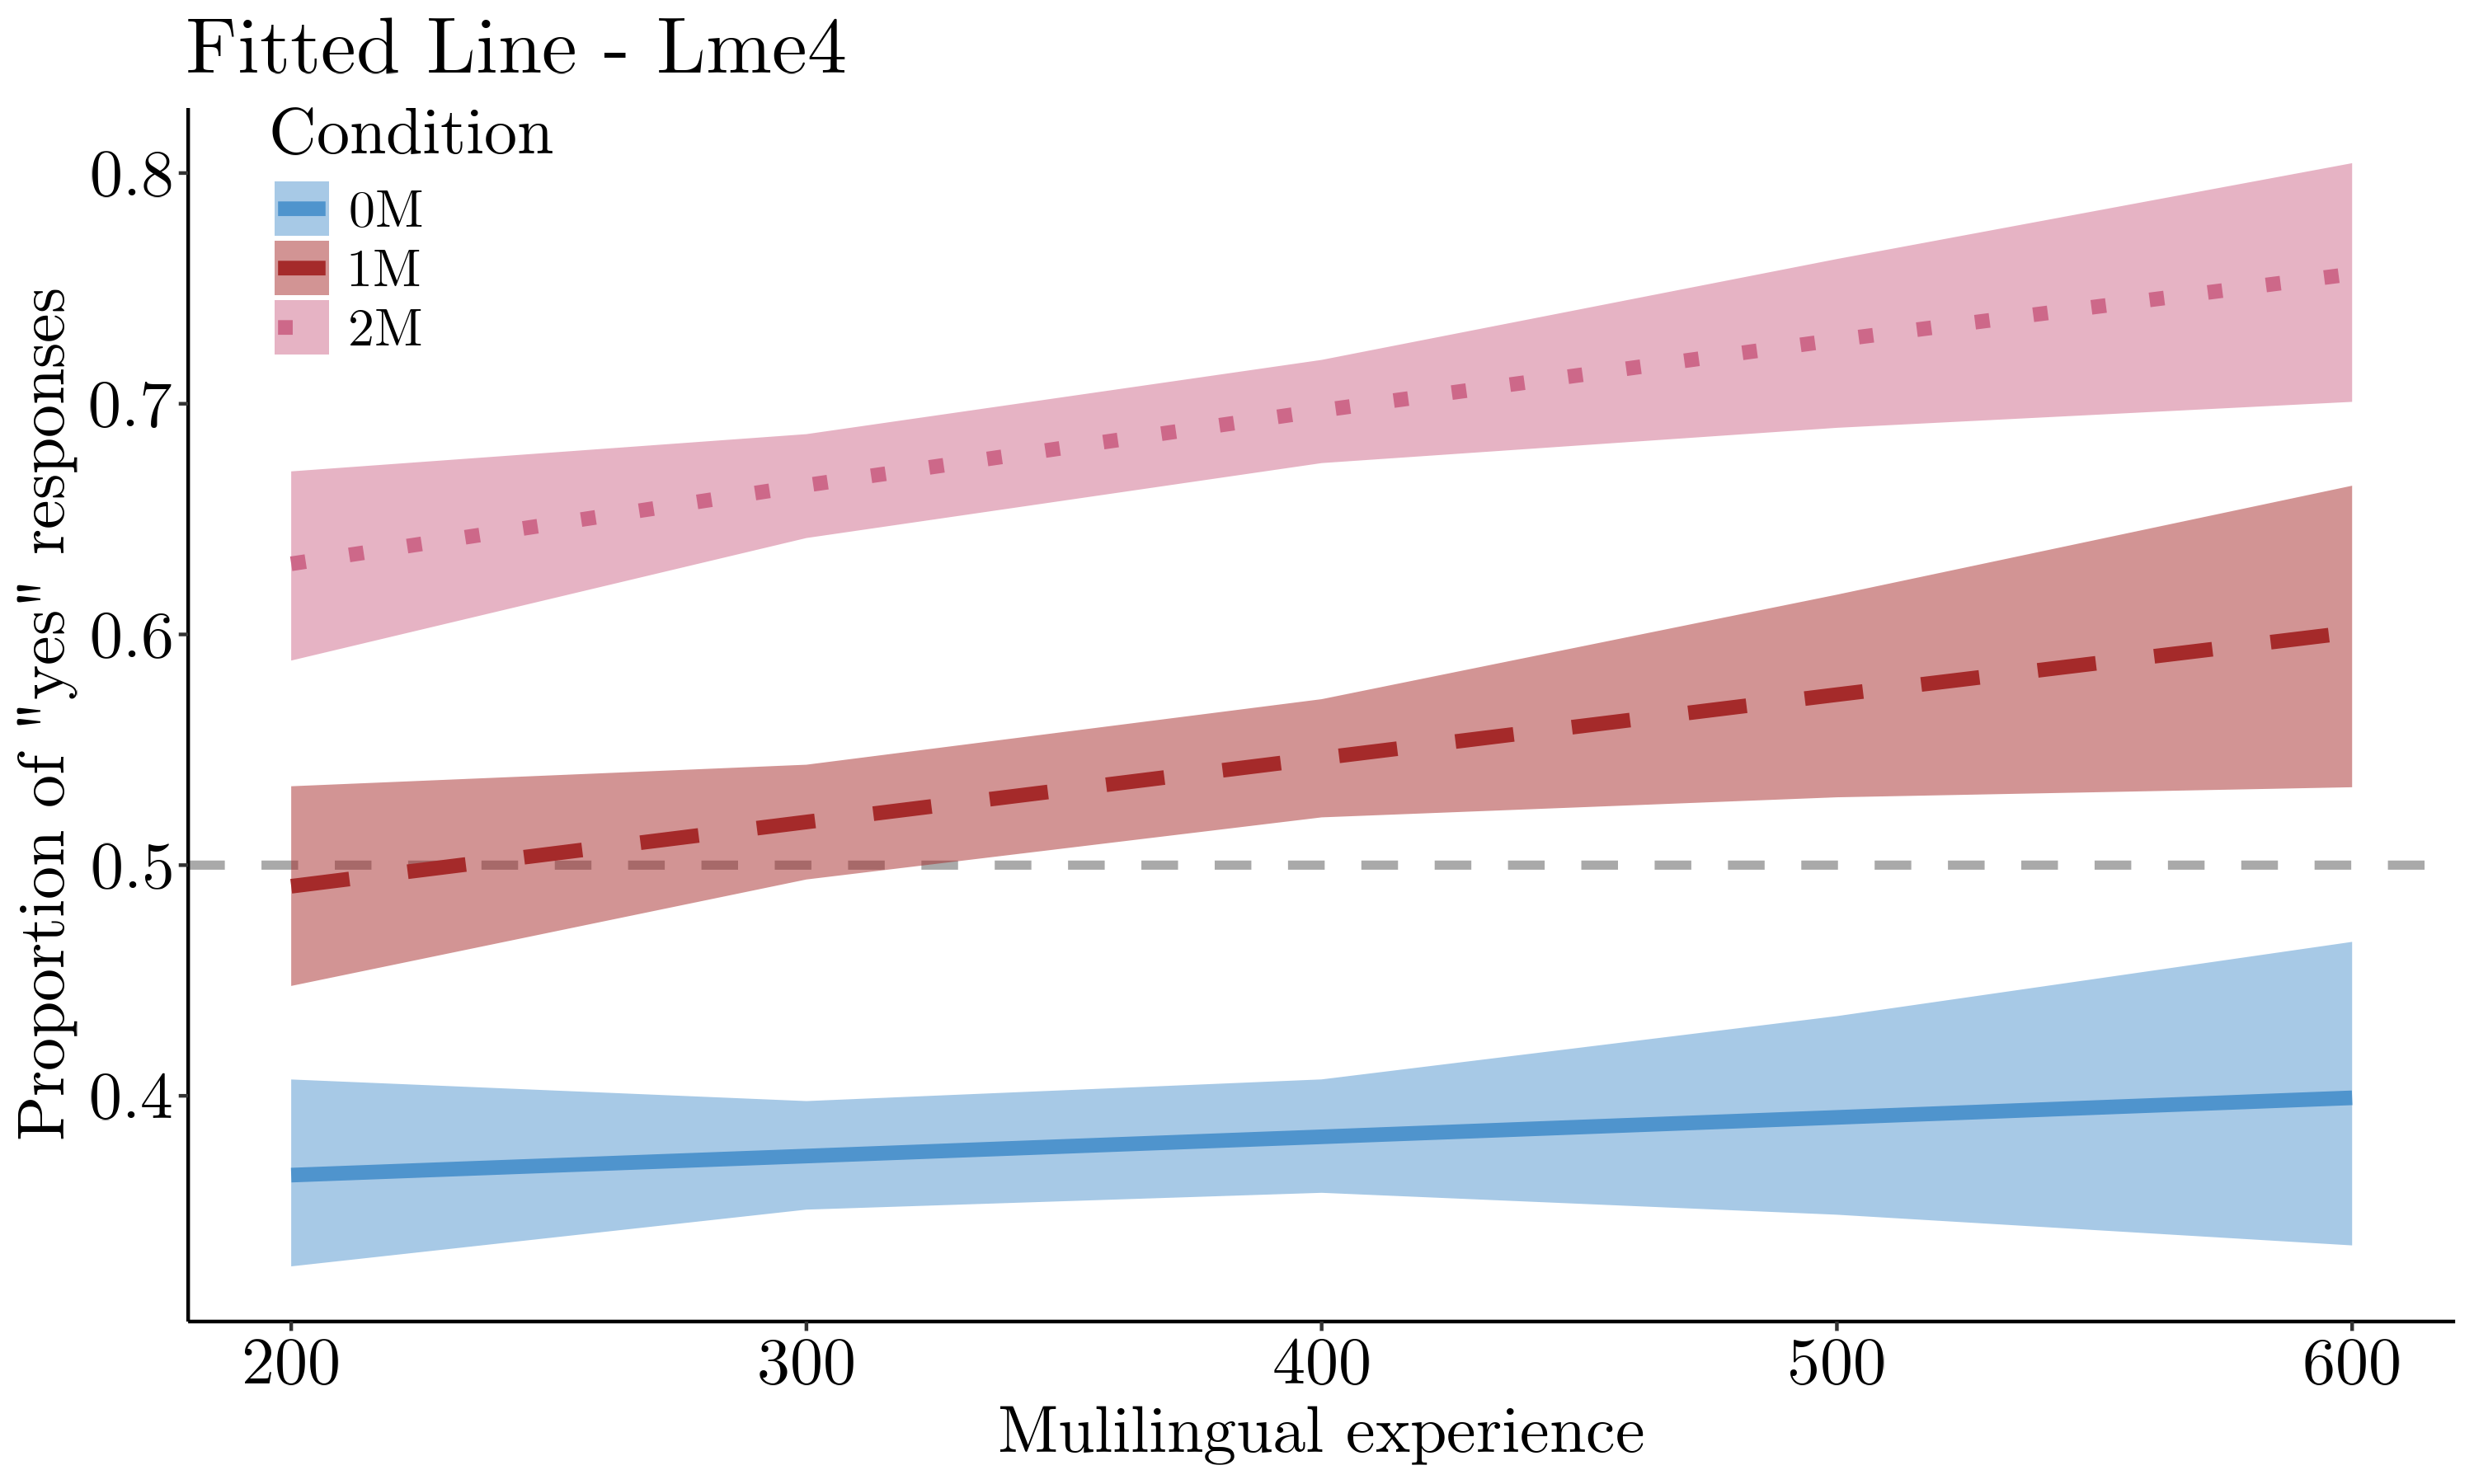
\includegraphics[width=0.99\textwidth]{Figures/exp3_yes_multiexp.png}
    \end{minipage}
    \begin{minipage}{0.49\linewidth}
        \centering
        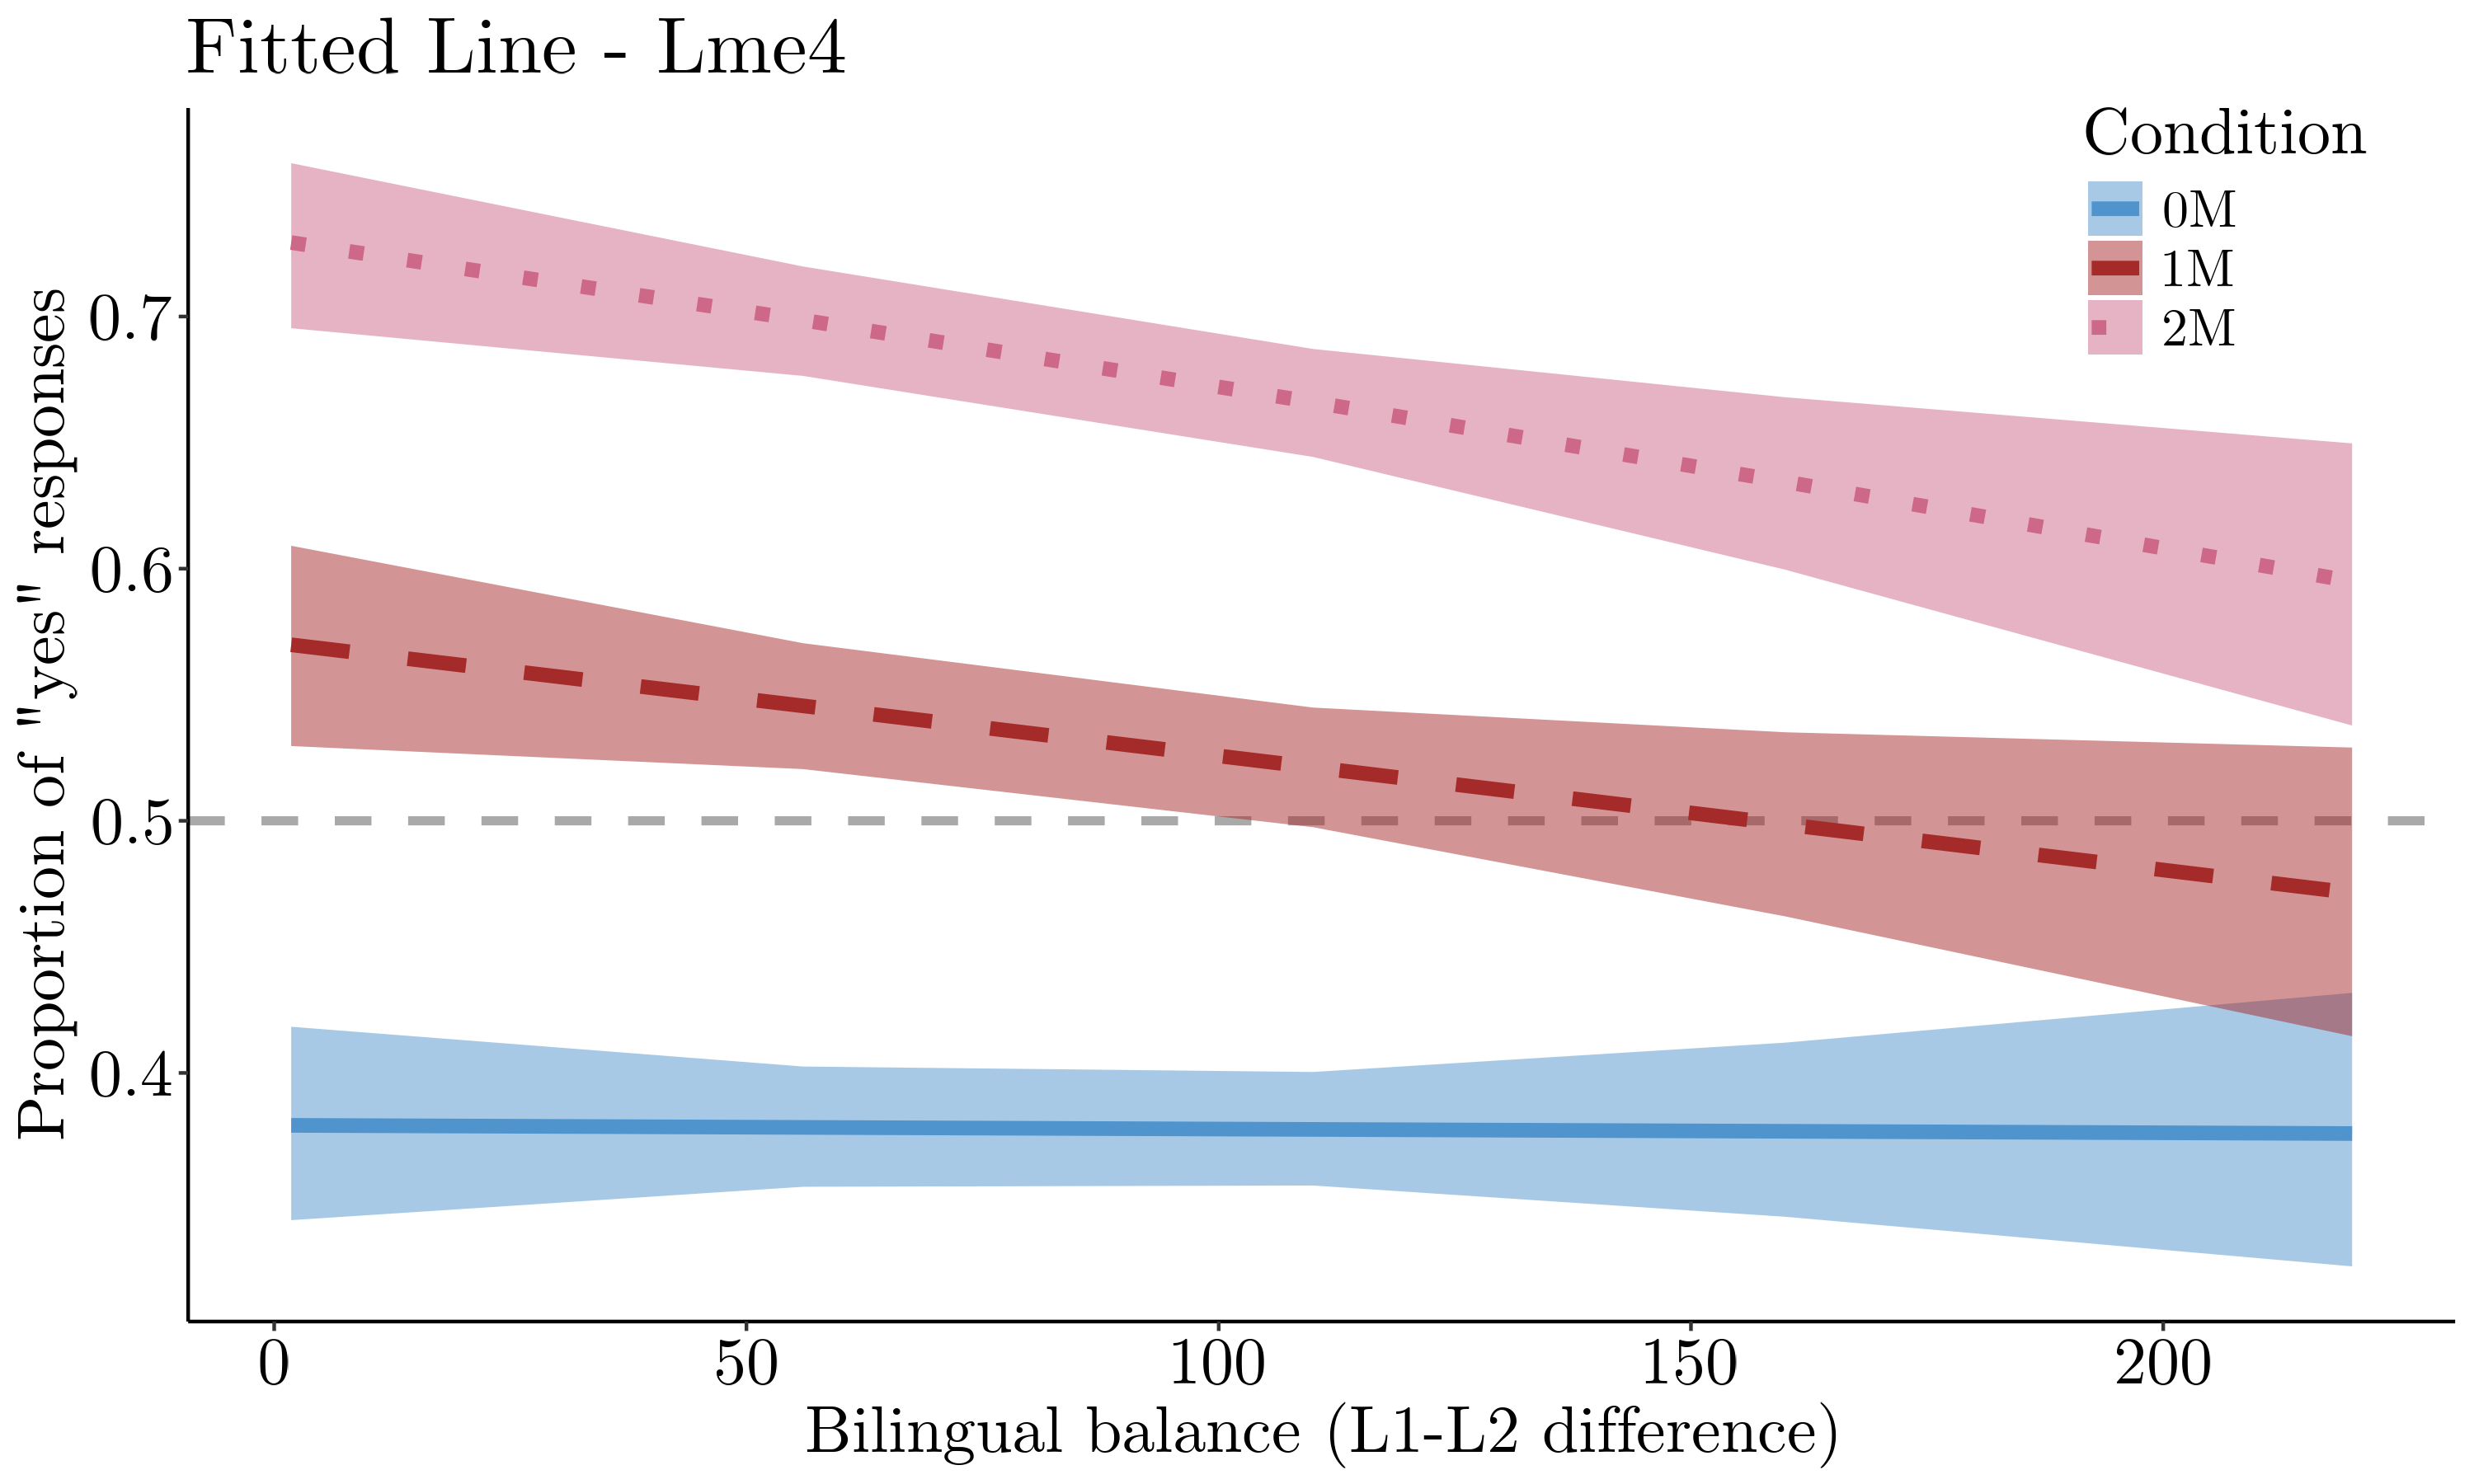
\includegraphics[width=0.99\textwidth]{Figures/exp3_yes_L1L2diff.png}
    \end{minipage}
    \begin{minipage}{0.99\linewidth}
        \centering
        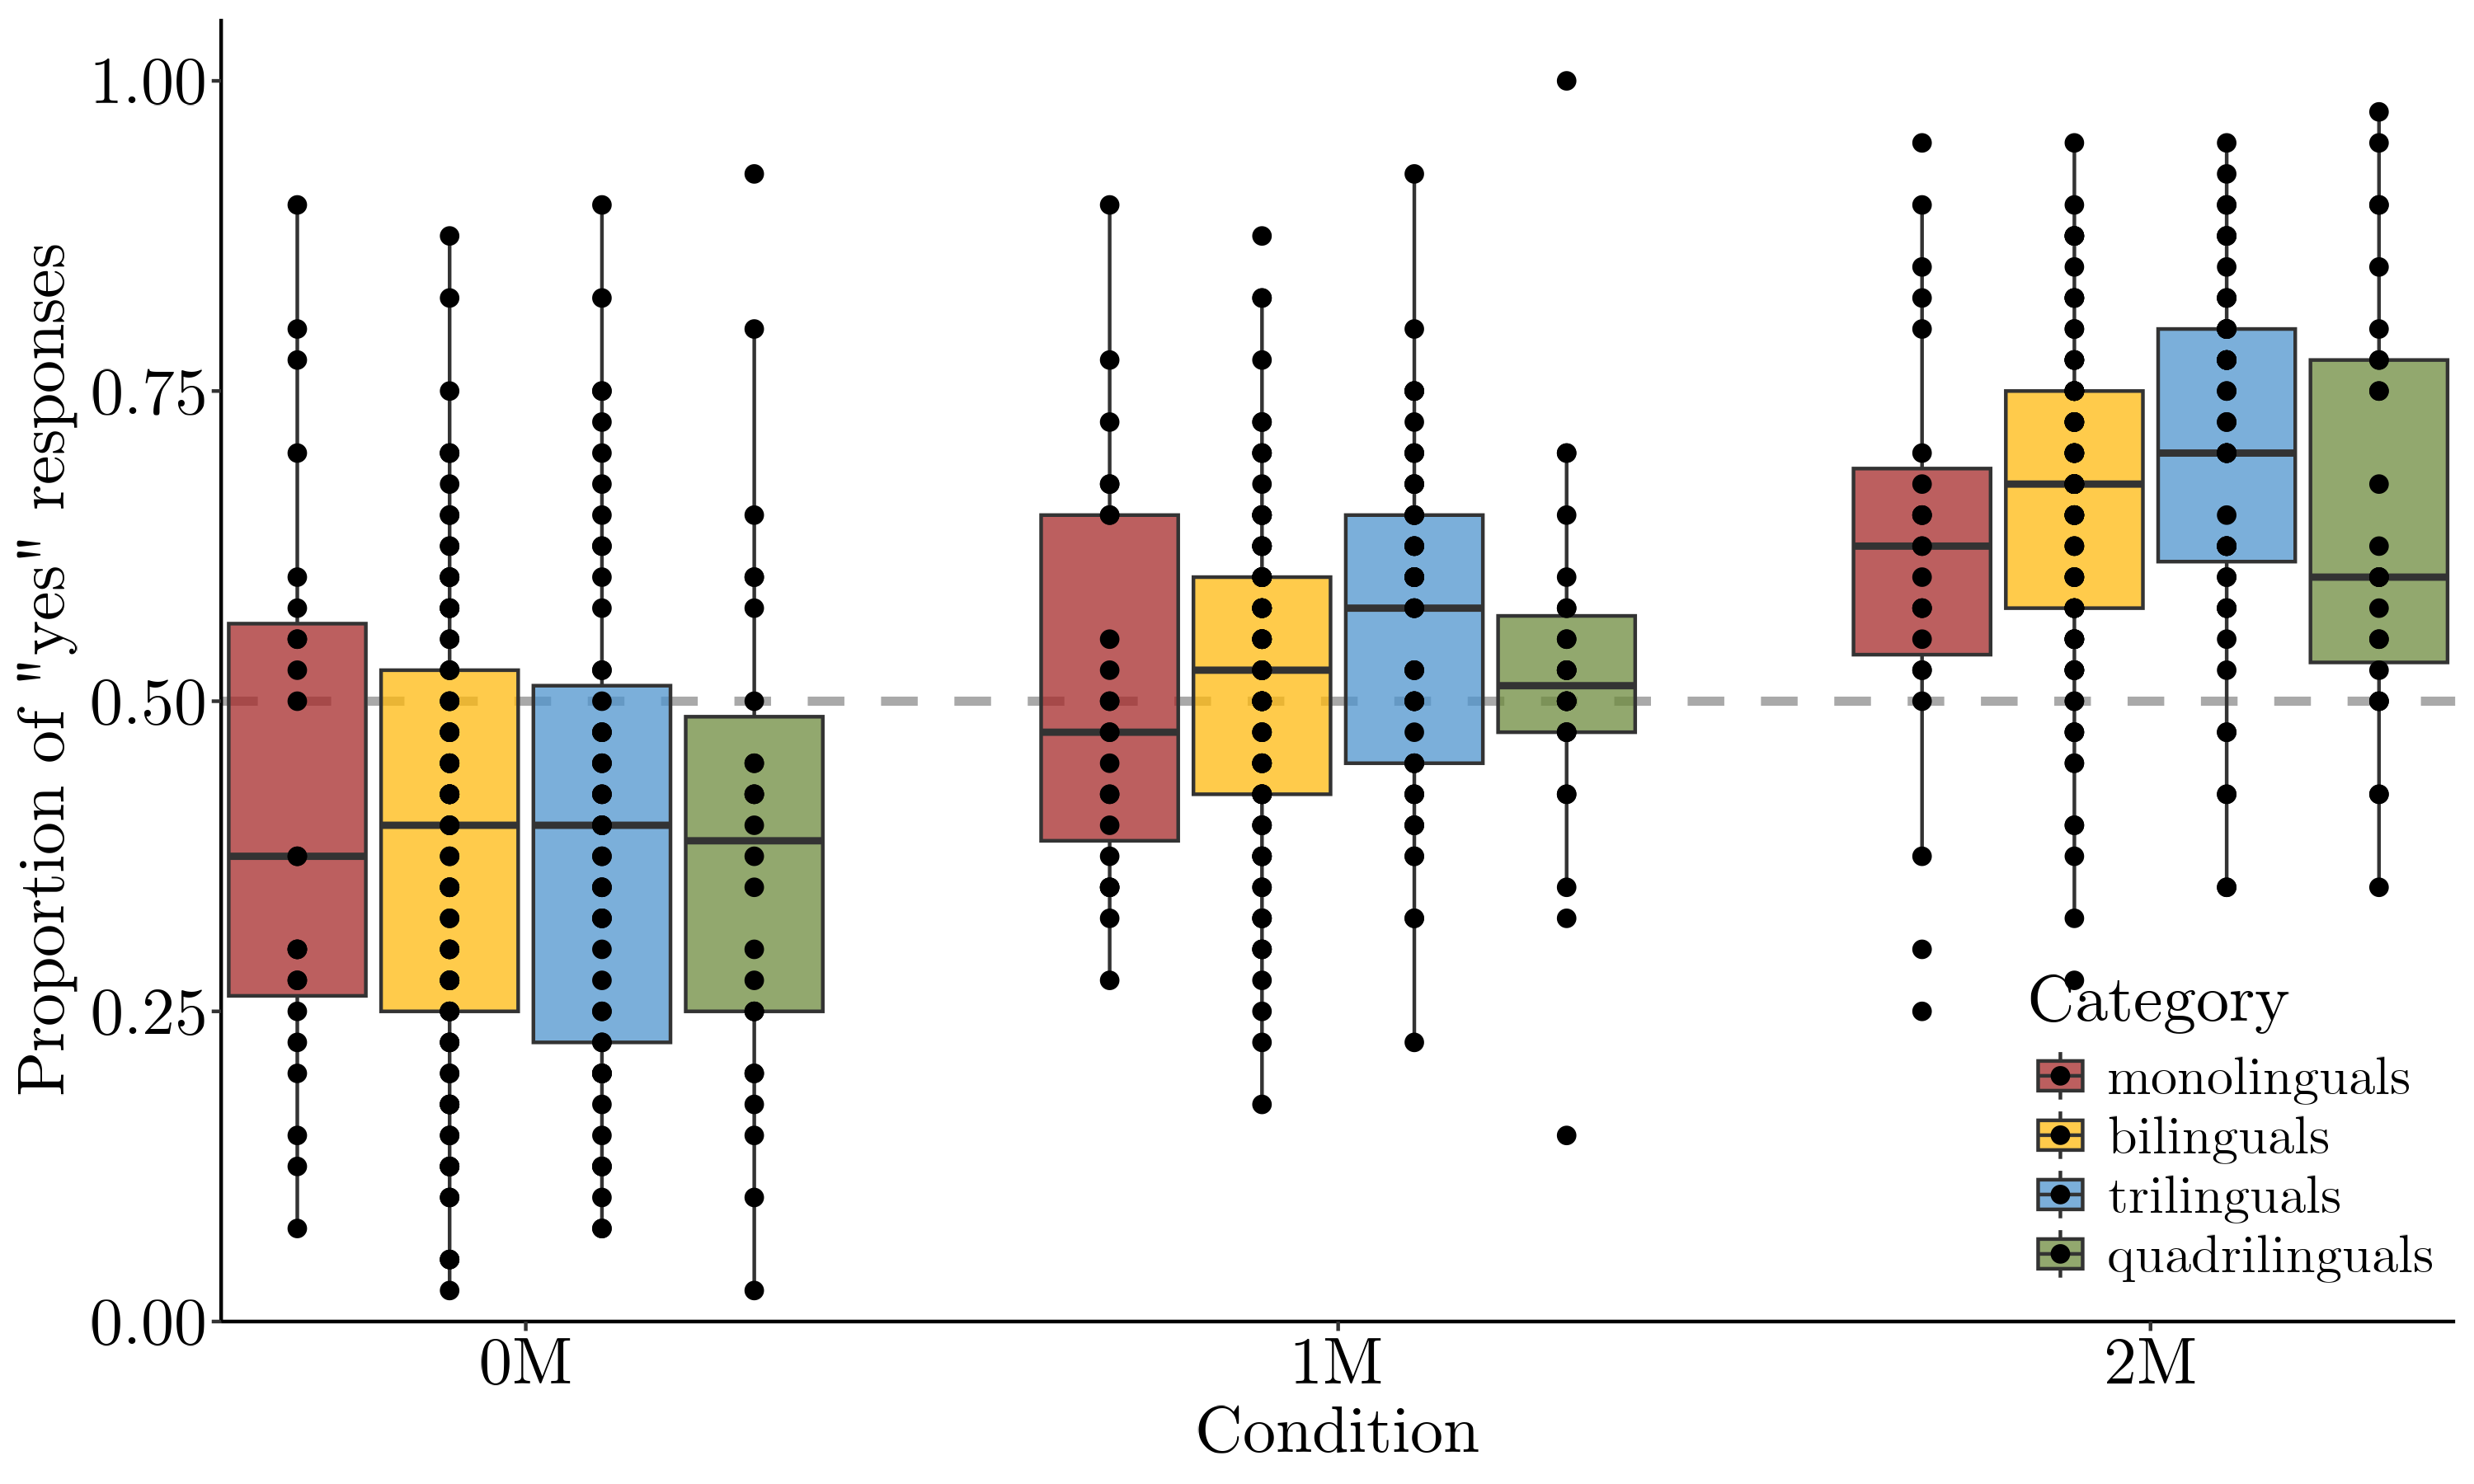
\includegraphics[width=0.99\textwidth]{Figures/exp3_yes_category.png}
    \end{minipage}
    \caption[]{\justifying Model estimates of the effect of multilingual experience (top left), bilingual balance (L1-L2 difference; top right), and multilingual category (bottom )  on ``yes'' responses, for the 0M (blue; solid), 1M (red; dashed), and 2M (pink; dotted) conditions. L1-L2 difference scores closer to 0 indicate a more balanced bilingual profile. Shaded areas around the lines indicate the 95\% confidence interval. The black dashed line at 0.5 indicates chance level.}
    \label{exp3_yes_multiexp/L1L2diff/category}
\end{figure}

\begin{table}[!htbp]
    \begin{center}
        \begin{tabular}{@{}lllll@{}}
            \toprule
            \multicolumn{5}{l}{\textbf{``yes'' responses across conditions}} \\ \midrule
            & \textbf{$\beta$} & \textbf{SE} & \textbf{z-value} & \textbf{p-value} \\ \midrule
            Cosine similarity & 3.30 & 1.26 & 2.61 & 0.009 \\ \midrule
            Women & -0.25 & 0.10 & -2.45 & 0.01 \\ \midrule
            Women$\ast$1M & 0.15 & 0.08 & 1.98 & 0.047 \\ \midrule
            Women$\ast$2M & 0.18 & 0.08 & 2.29 & 0.02 \\ \midrule
            PC1 (L4)$\ast$2M & -0.11 & 0.04 & -3.05 & 0.002 \\ \midrule
            PC2 (L1 vs L2 use)$\ast$1M & 0.10 & 0.03 & 2.89 & 0.004 \\ \midrule
            PC2 (L1 vs L2 use)$\ast$2M & 0.19 & 0.04 & 5.25 & 1.5e$^{-7}$ \\ \midrule
            Entropy$\ast$1M & 0.18 & 0.07 & 2.71 & 0.007 \\ \midrule
            Entropy$\ast$2M & 0.28 & 0.07 & 4.04 & 0.00005 \\ \midrule
            Multilingual experience$\ast$2M & 0.10 & 0.04 & 2.71 & 0.007 \\ \midrule
            L1-L2 difference$\ast$1M & -0.10 & 0.03 & -2.77 & 0.006 \\ \midrule
            L1-L2 difference$\ast$2M & -0.15 & 0.04 & -4.20 & 0.00003 \\ \midrule
            Bilinguals$\ast$2M & 0.24 & 0.11 & 2.07 & 0.04 \\ \midrule
            Trilinguals$\ast$1M & 0.36 & 0.12 & 3.01 & 0.003 \\ \midrule
            Trilinguals$\ast$2M & 0.54 & 0.12 & 4.39 & 0.00001 \\ \midrule
            Quadrilinguals$\ast$2M & 0.32 & 0.14 & 2.25 & 0.02 \\ \midrule
            \bottomrule
        \end{tabular}
    \end{center}
    \caption{Summary of experiment 3 mixed modelling statistics of ``yes'' responses across conditions, for significant variables.}
    \label{exp3_yes_summary}
\end{table}
\break

\noindent
\underline{2M performance}

\noindent
Isolating focus on the key 2M condition, there were some main effects on ``yes'' responses in that condition. More L2 use compared to L1 use led to more ``yes'' responses in the 2M condition (PC2 main effect $\beta$ = 0.18, z = 3.10, p = 0.002). These responses were also increased for participants with more multilingual experience (multilingual experience main effect $\beta$ = 015, z = 2.59, p = 0.0098). Those with more balance, either bilingual or multilingual, responded ``yes'' more as well (L1-L2 difference main effect $\beta$ = -0.15, z = -2.74, p = 0.006; cosine similarity main effect $\beta$ = 0.11, z = 1.99, p = 0.047). In this version of the experiment, participants who spoke language with different scripts also tended to respond ``yes'' more often in the 2M condition (script main effect $\beta$ = 0.24, z = 2.14, p = 0.03).

\begin{figure}[!htbp]
    \begin{minipage}{0.49\linewidth}
        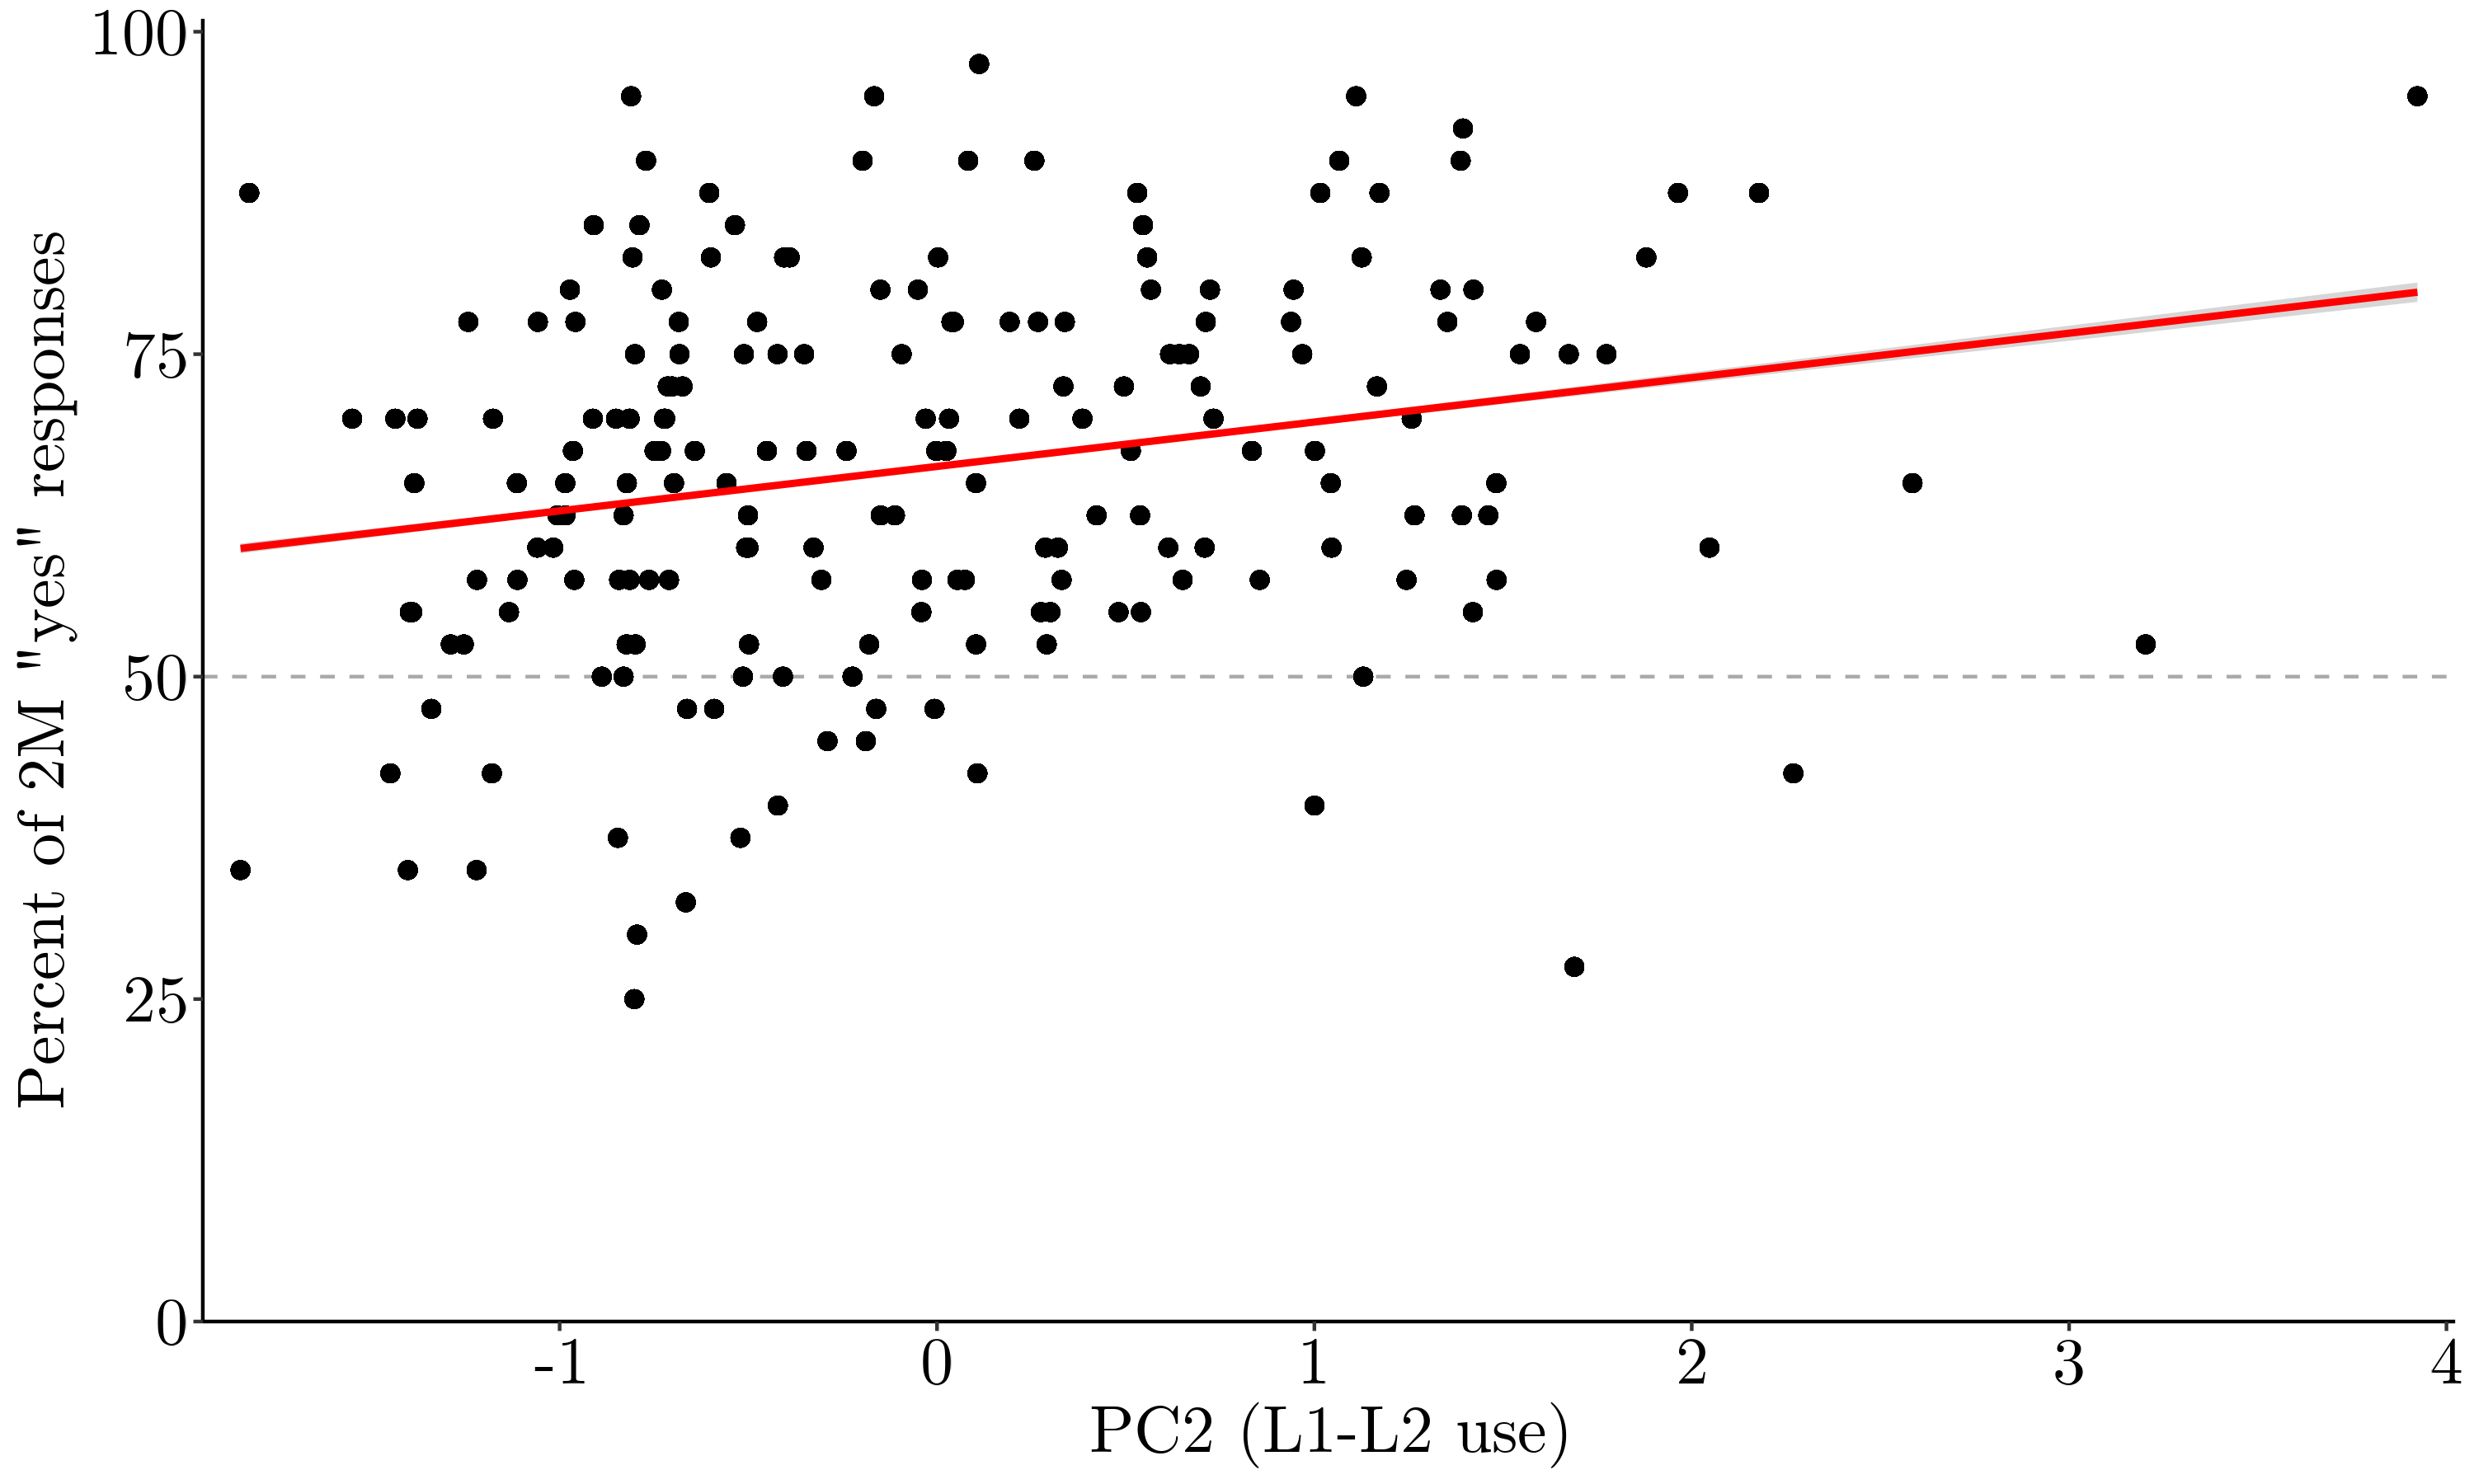
\includegraphics[width=0.99\textwidth]{Figures/exp3_2M_yes_PC2.png}
    \end{minipage}
    \begin{minipage}{0.49\linewidth}
        \centering
        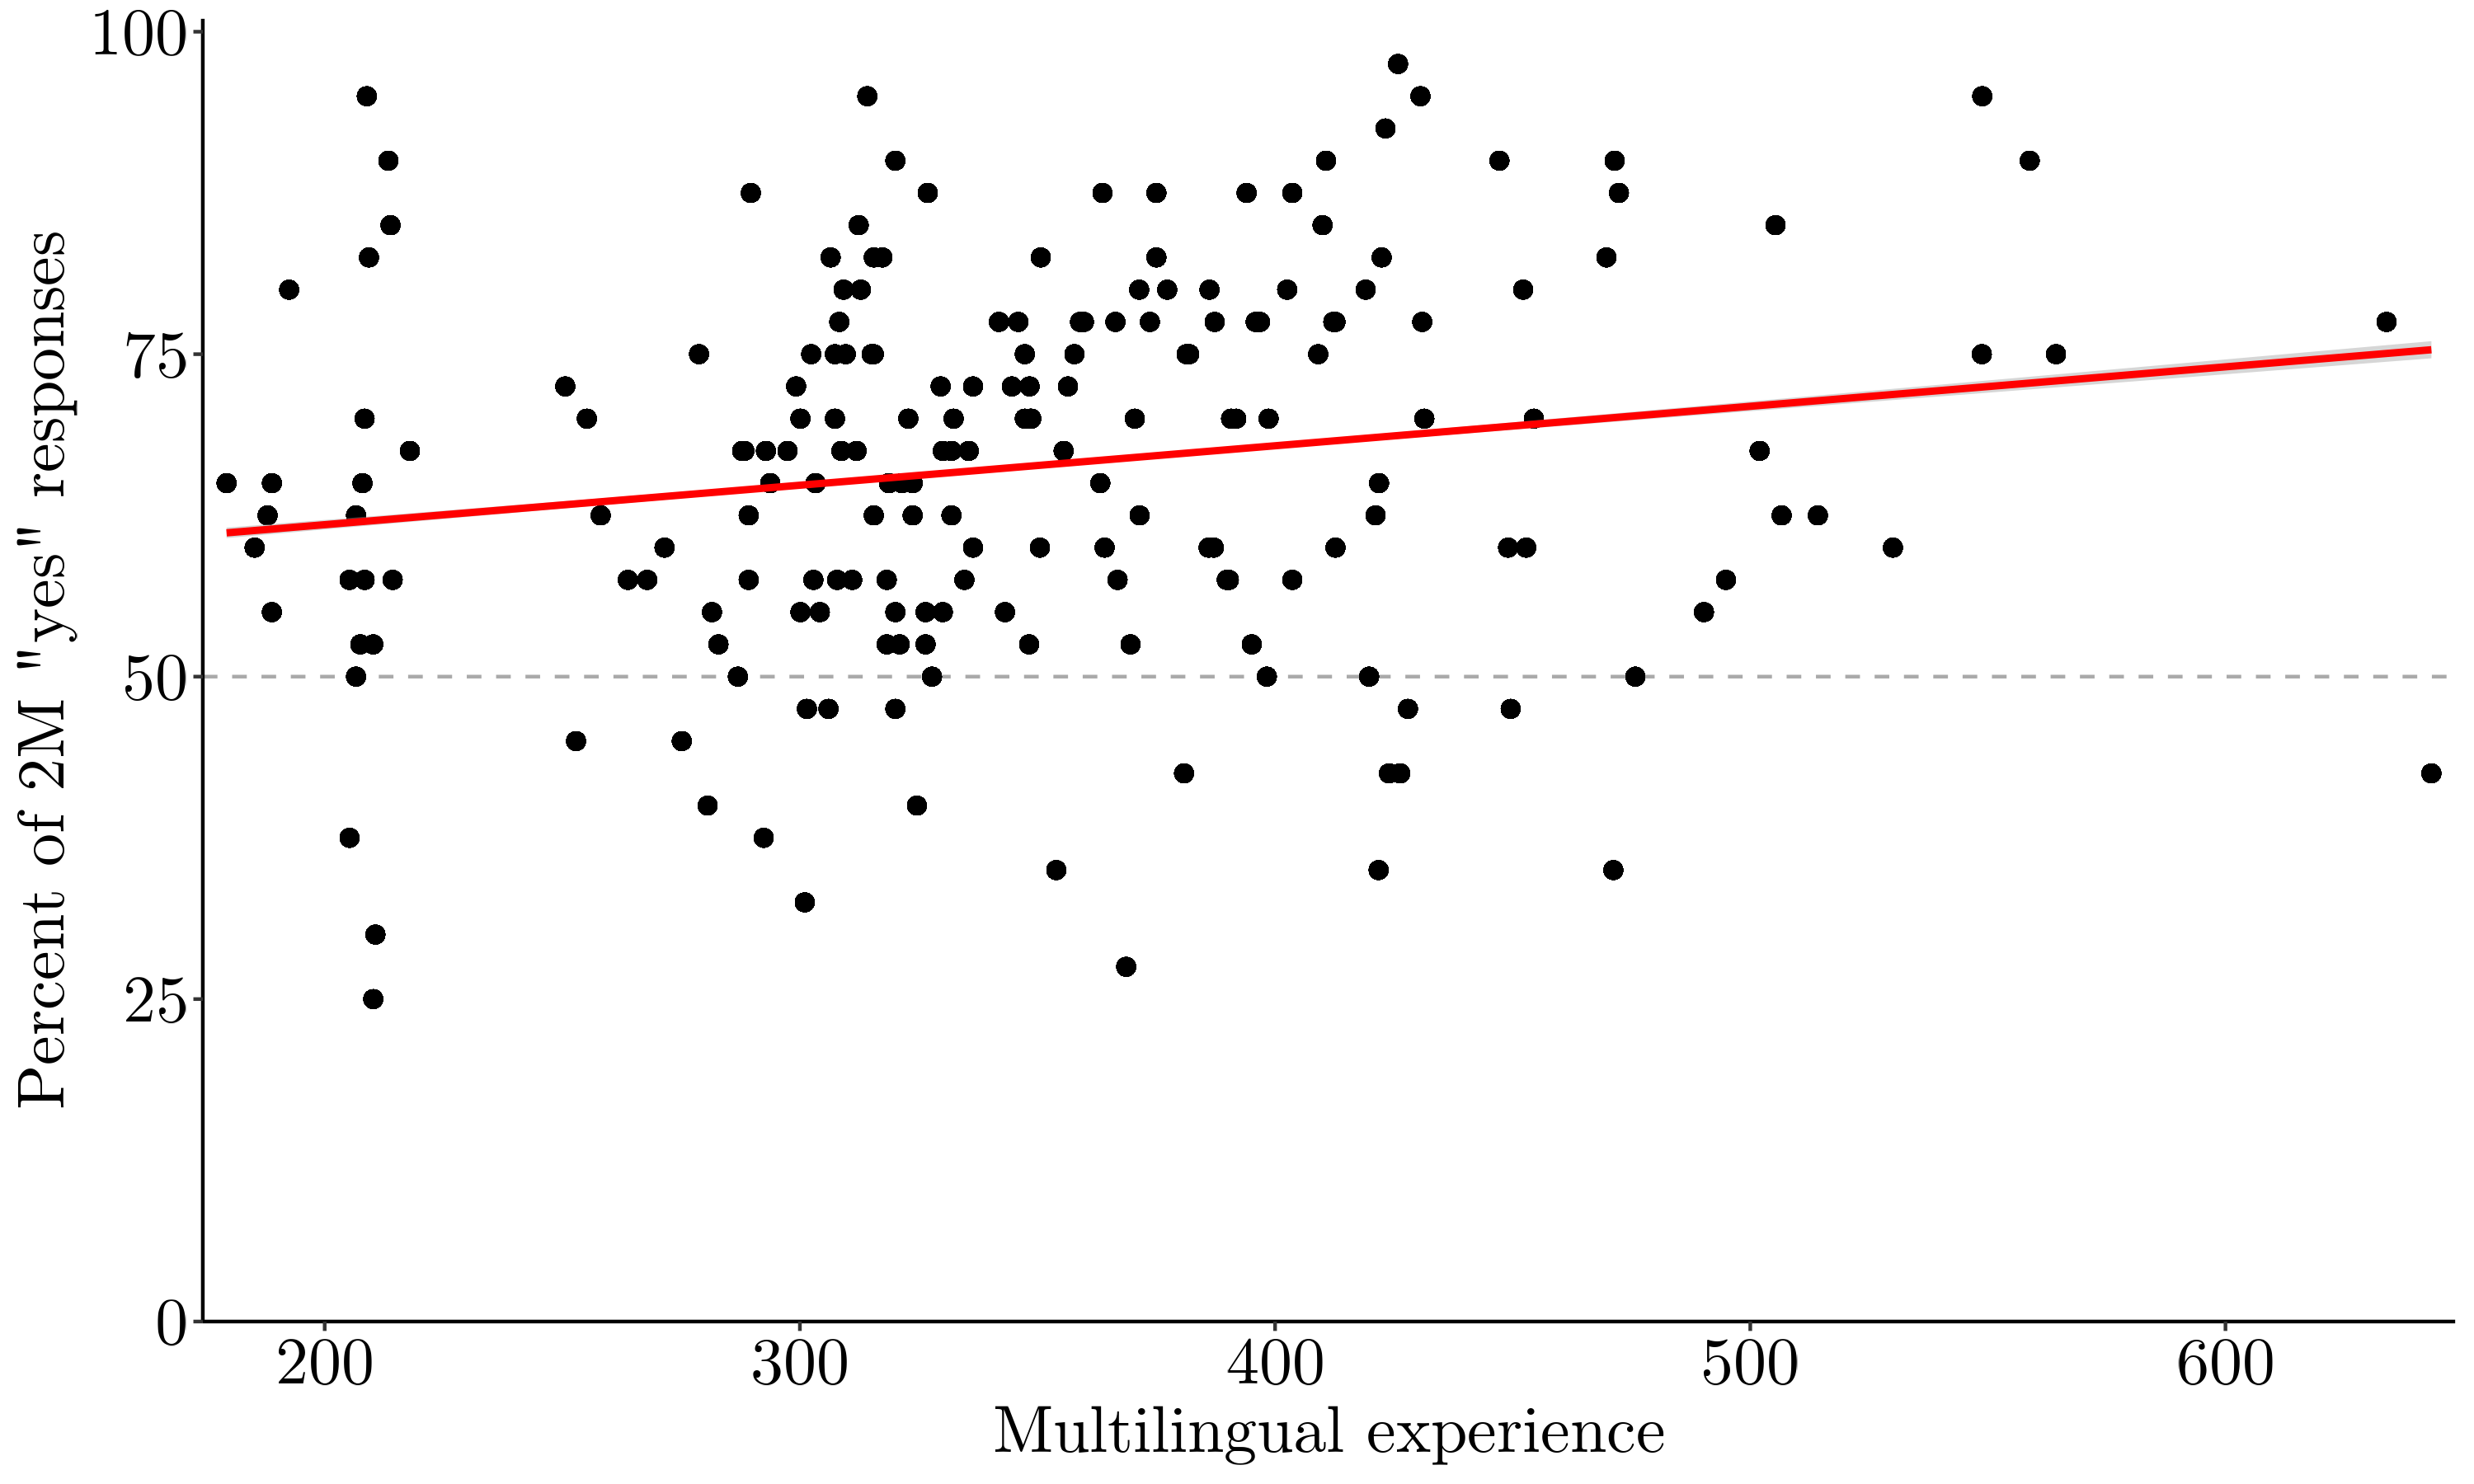
\includegraphics[width=0.99\textwidth]{Figures/exp3_2M_yes_multiexp.png}
    \end{minipage}
    \begin{minipage}{0.49\linewidth}
        \centering
        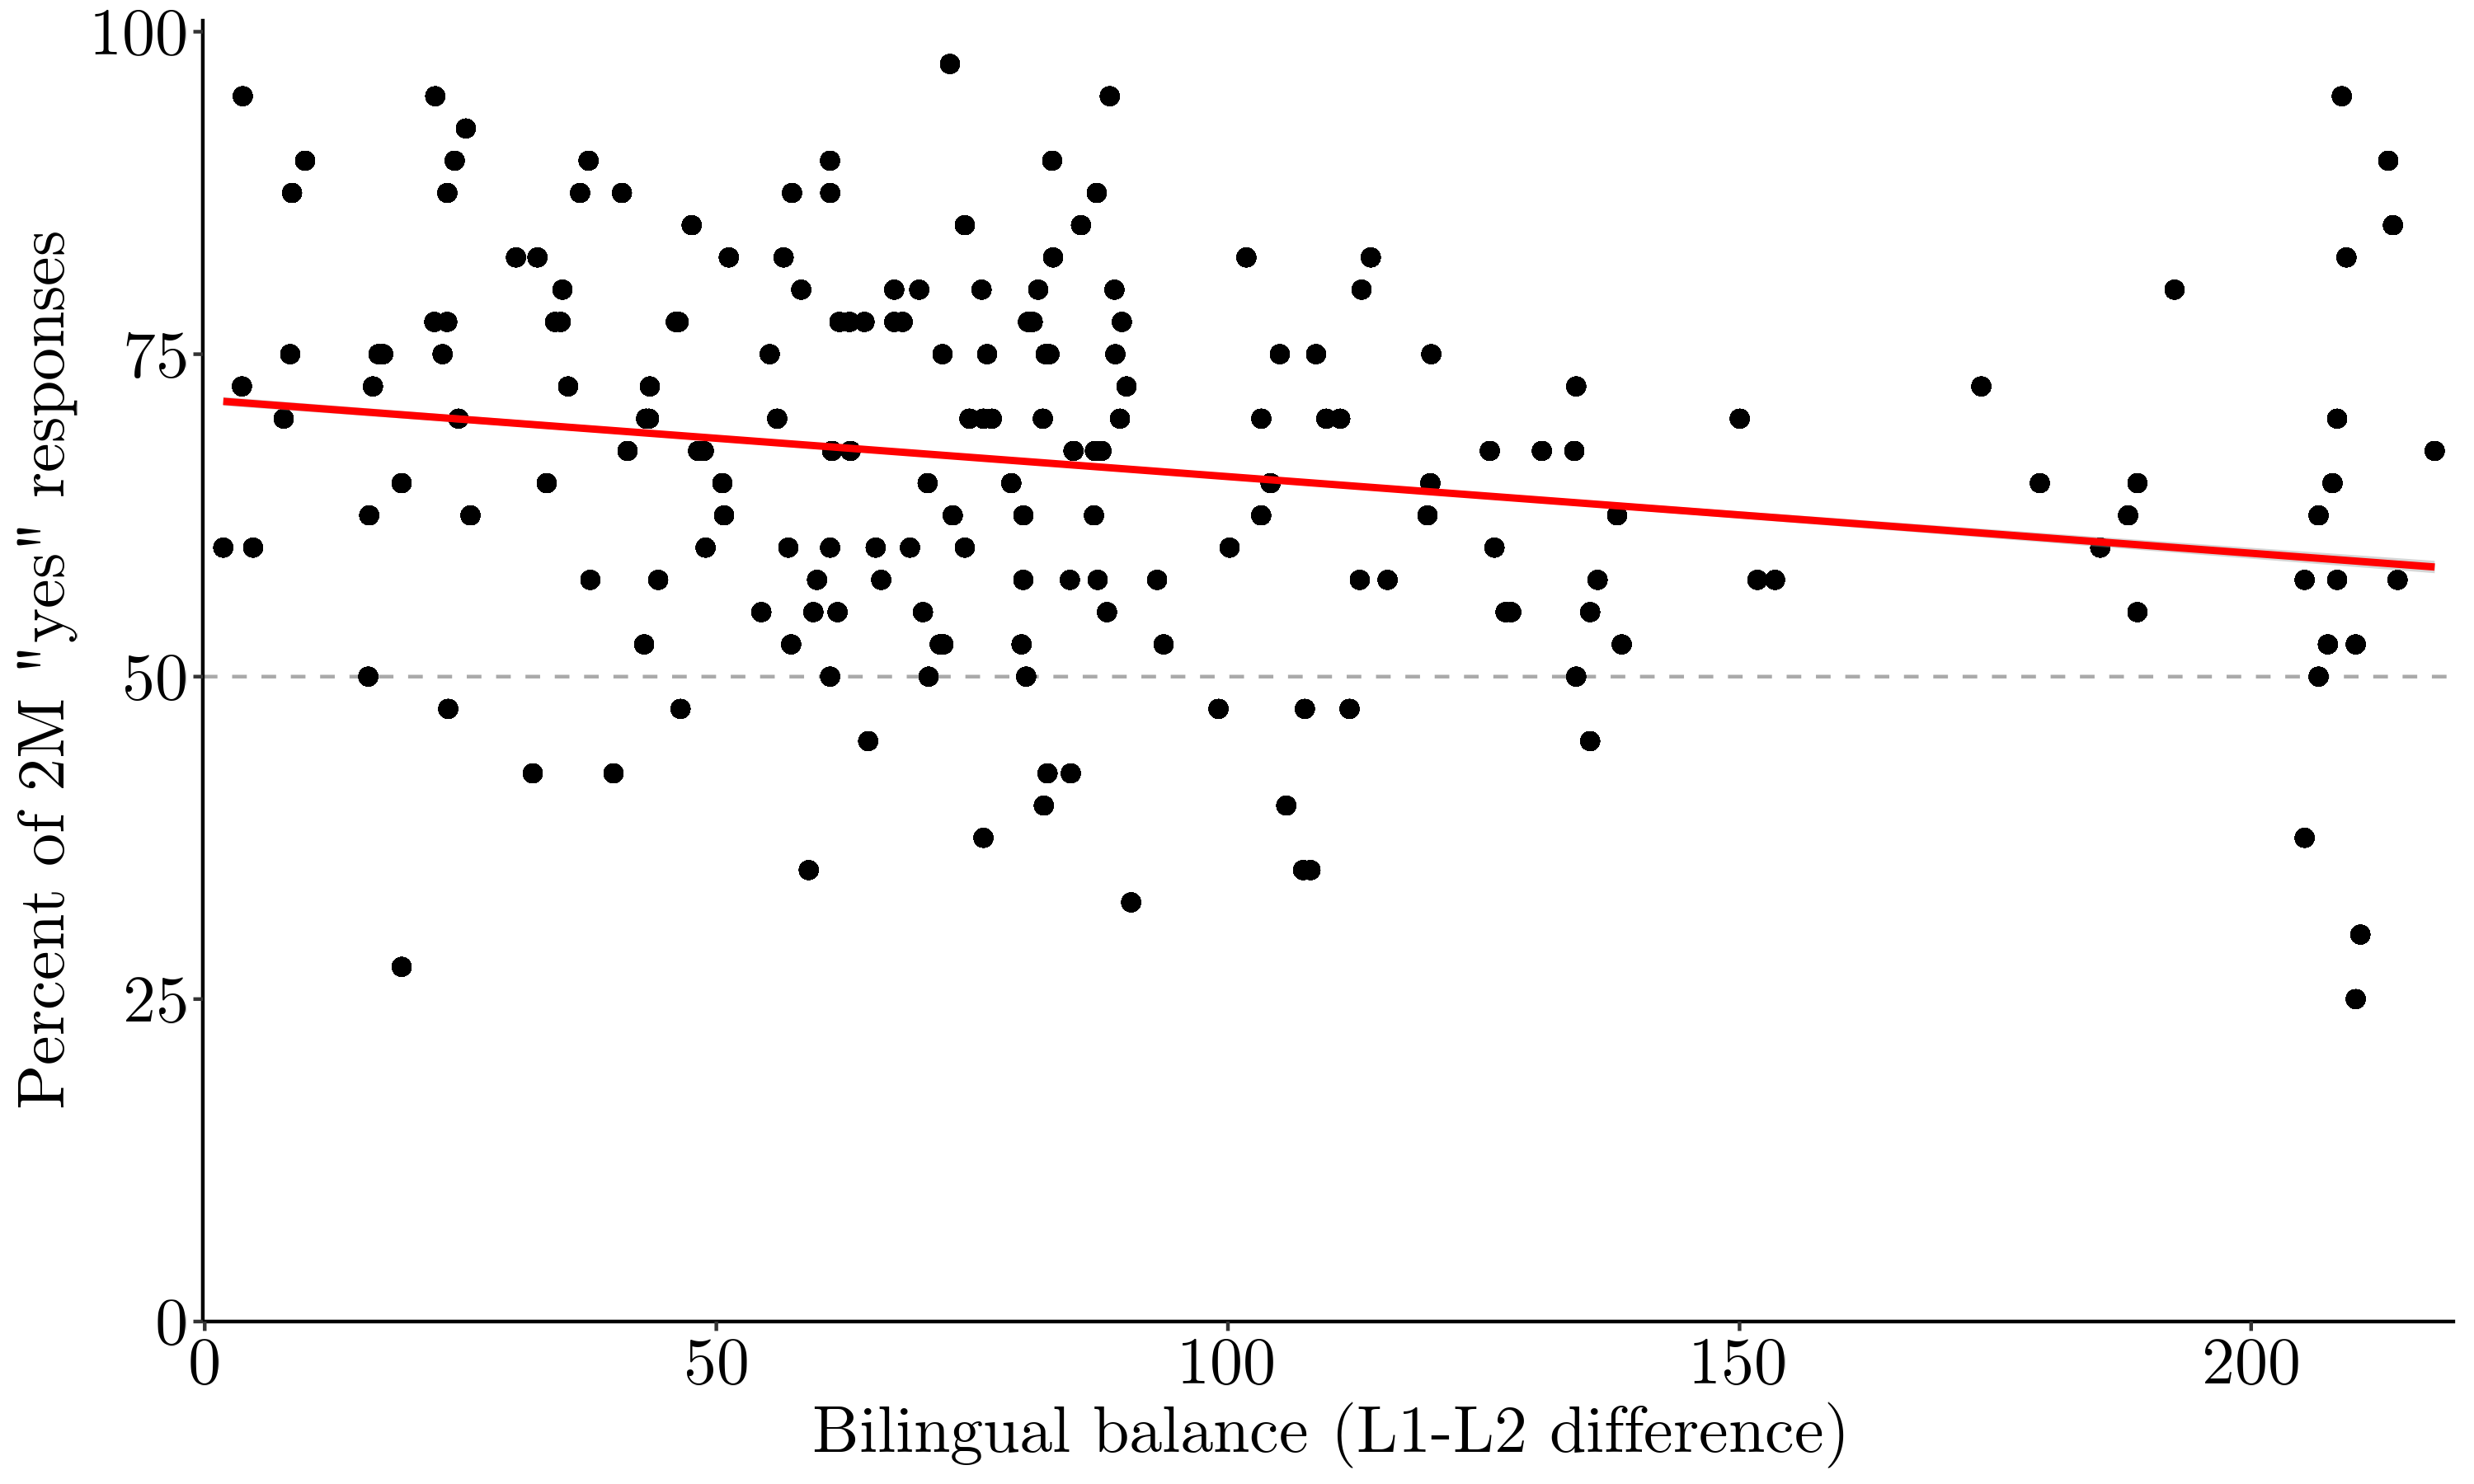
\includegraphics[width=0.99\textwidth]{Figures/exp3_2M_yes_L1L2diff.png}
    \end{minipage}
    \begin{minipage}{0.49\linewidth}
        \centering
        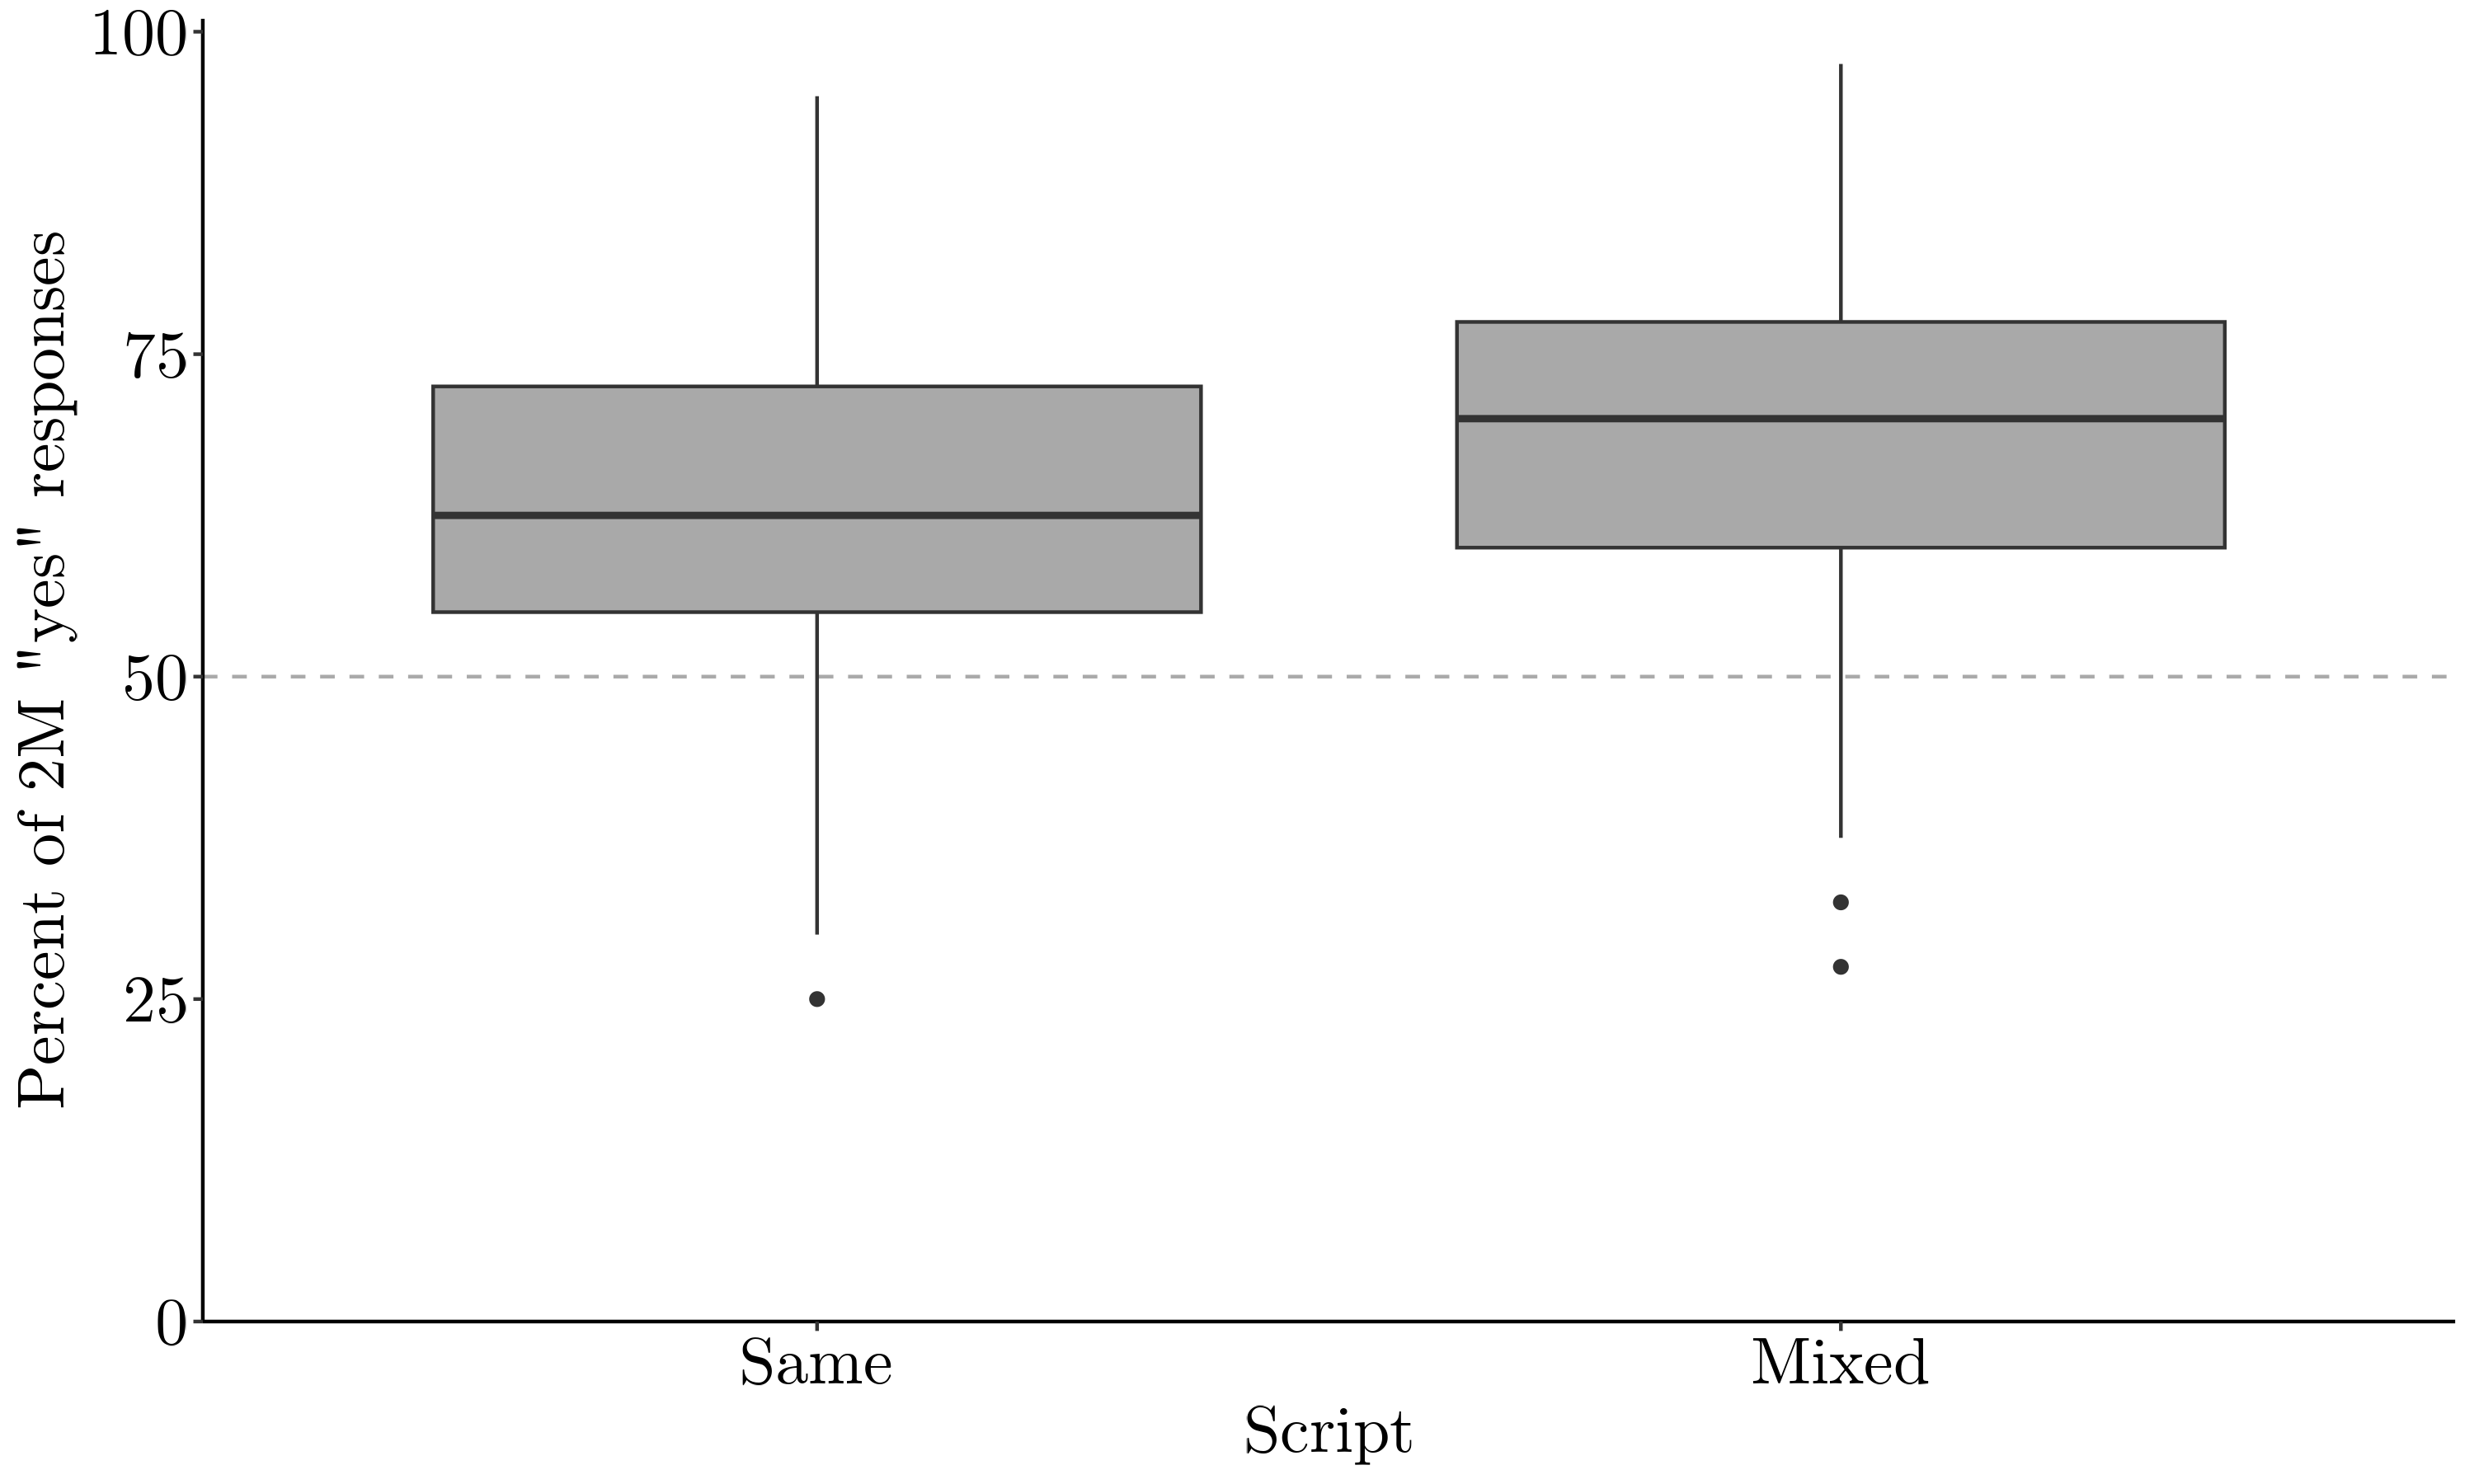
\includegraphics[width=0.99\textwidth]{Figures/exp3_2M_yes_script.png}
    \end{minipage}
    \caption[]{\justifying Plots of the percent of ``yes'' responses in the 2M condition as a function of PC2 (L2 vs L1 use; top left), multilingual experience (top right), bilingual balance (L1-L2 difference; bottom right), and script type (bottom right). Higher levels of PC2 means more L2 rather than L1 use. Lower levels of L1-L2 difference indicate more balanced profiles. The dashed line at 50\% indicate chance level.}
    \label{exp2_2Myes_PC2/multiexp/L1L2diff/script}
\end{figure}

\begin{figure}[!htbp]
    \begin{center}
        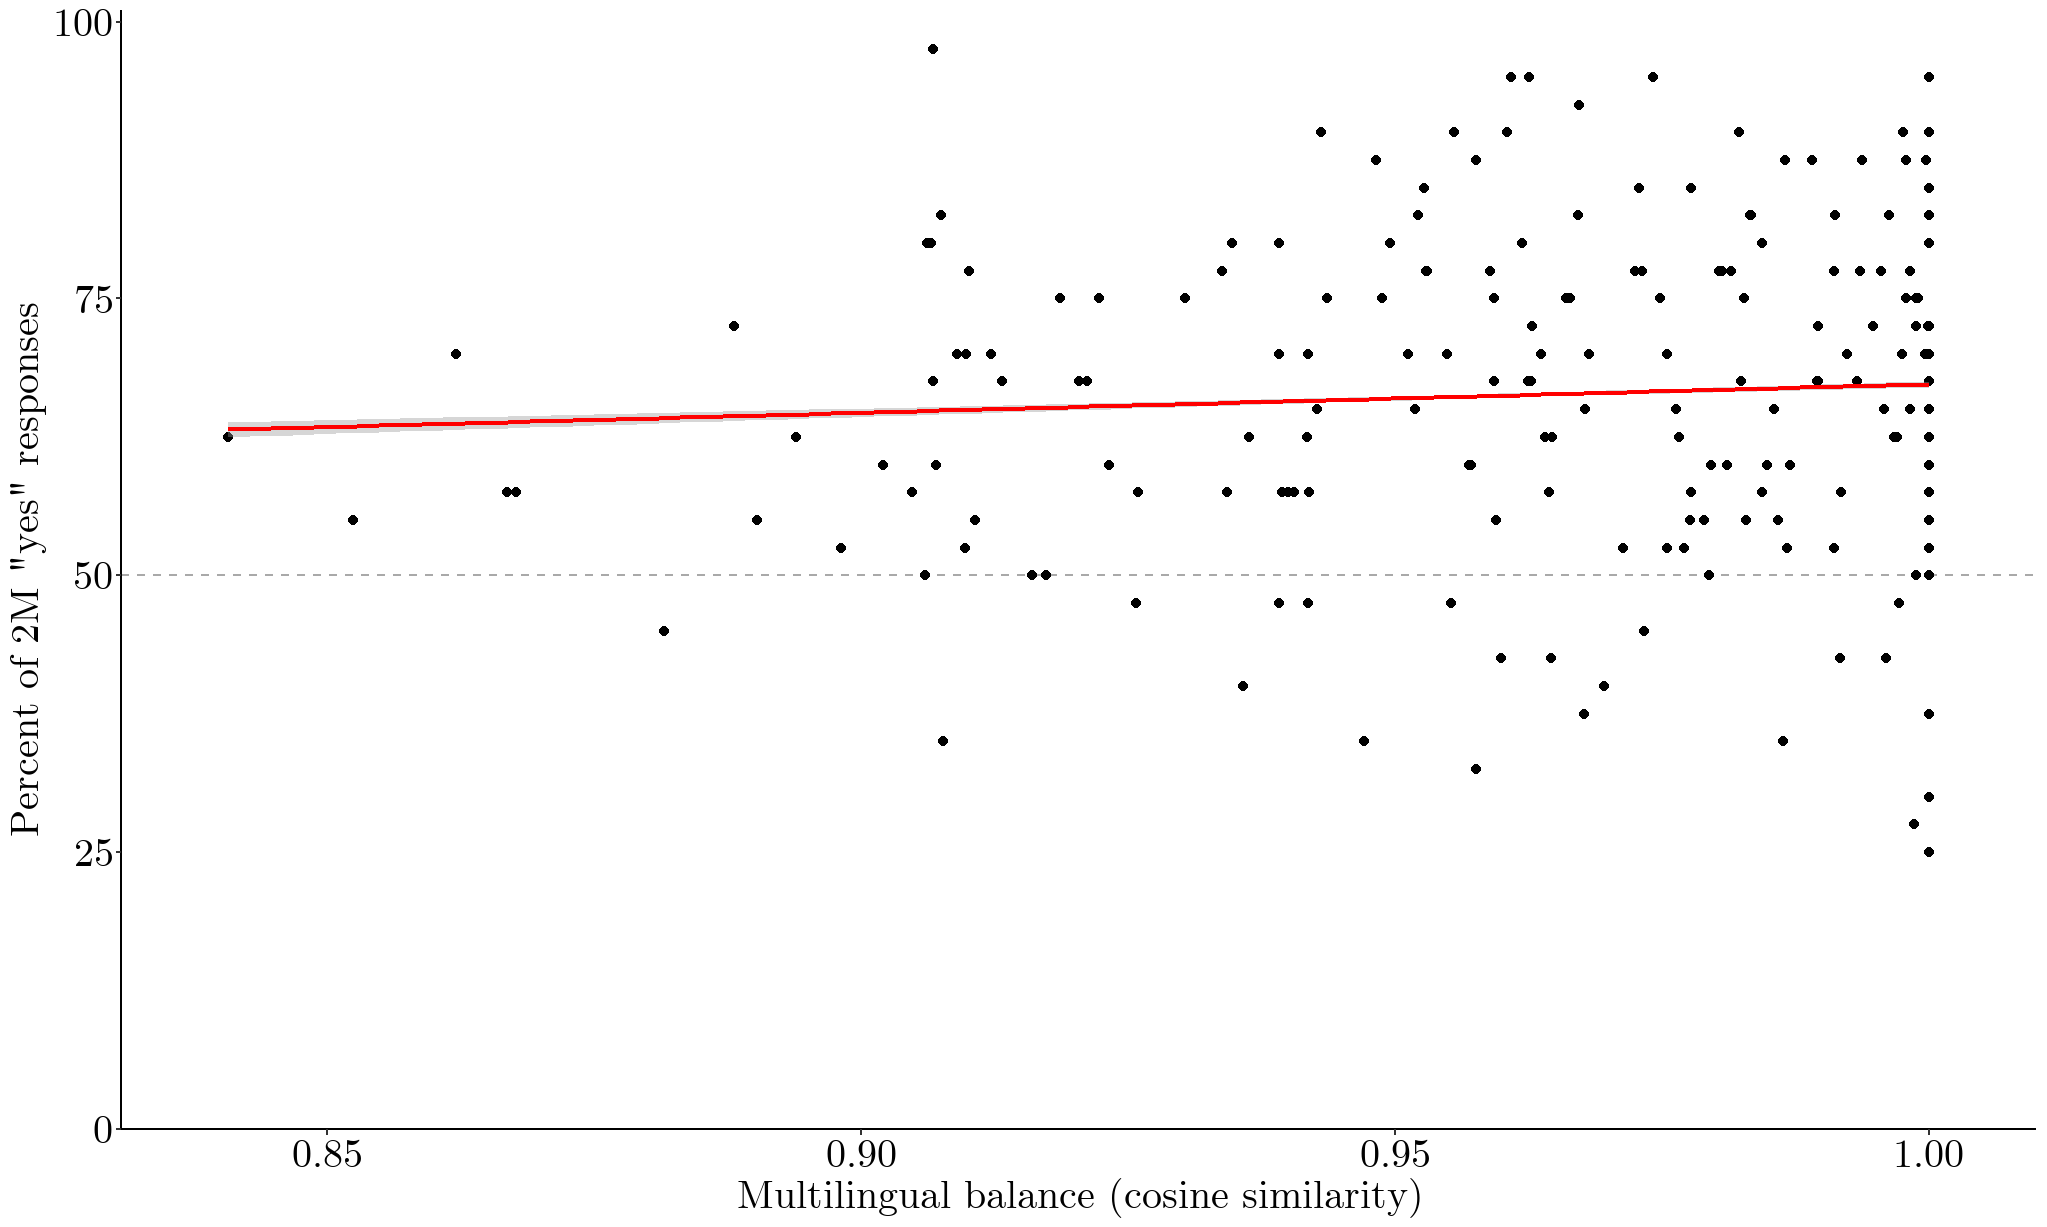
\includegraphics[width=0.6\textwidth]{Figures/exp3_2M_yes_cossim.png}
    \end{center}
    \caption[]{\justifying Plot of the effect of multilingual balance (cosine similarity) on 2M ``yes'' responses. Cosine similarity scores closer to 1 indicate more balance across a participants' languages. The dashed line at 50\% indicates chance level.}
    \label{exp3_2Myes_cossim}
\end{figure}

Crucially, three variables also predicted 2M accuracy. Most interesting given the results from the previous experiment, multilingual balance (cosine similarity) was once again a significant predictor of 2M accuracy (cosine similarity interaction $\beta$ = -0.13, z = -2.56, p = 0.01). However, in this version of the experiment, this effect preserved its significance when calculated without monolingual participants (cosine similarity interaction $\beta$ = -0.11, z = -2.02, p = 0.04). This relationship wa, however, in an unexpected direction: more balanced multilinguals were less accurate. Exploratory analyses found the same pattern of results when calculating cosine similarity using language use scores as opposed to overall language scores, as is sometimes done in past literature (use cosine similarity $\beta$ = -0.11, z = -2.24, p = 0.03). This would indicate that the previously detailed cosine similarity effect might be influenced in this direction through its language use components. 

Finally, the bilingual group had significantly higher accuracy than monolinguals (bilingual interaction $\beta$ = 0.34, z = 2.06, p = 0.04). In order to ensure that this group's accuracy was also significantly above chance level instead of the linear model intercept, a post-hoc Student's t-test was conducted. This confirmed that this group performed above chance level (t(90) = 3.46, p = 0.0008, estimate = 0.52). 

\begin{figure}[!htbp]
    \begin{minipage}{0.49\linewidth}
        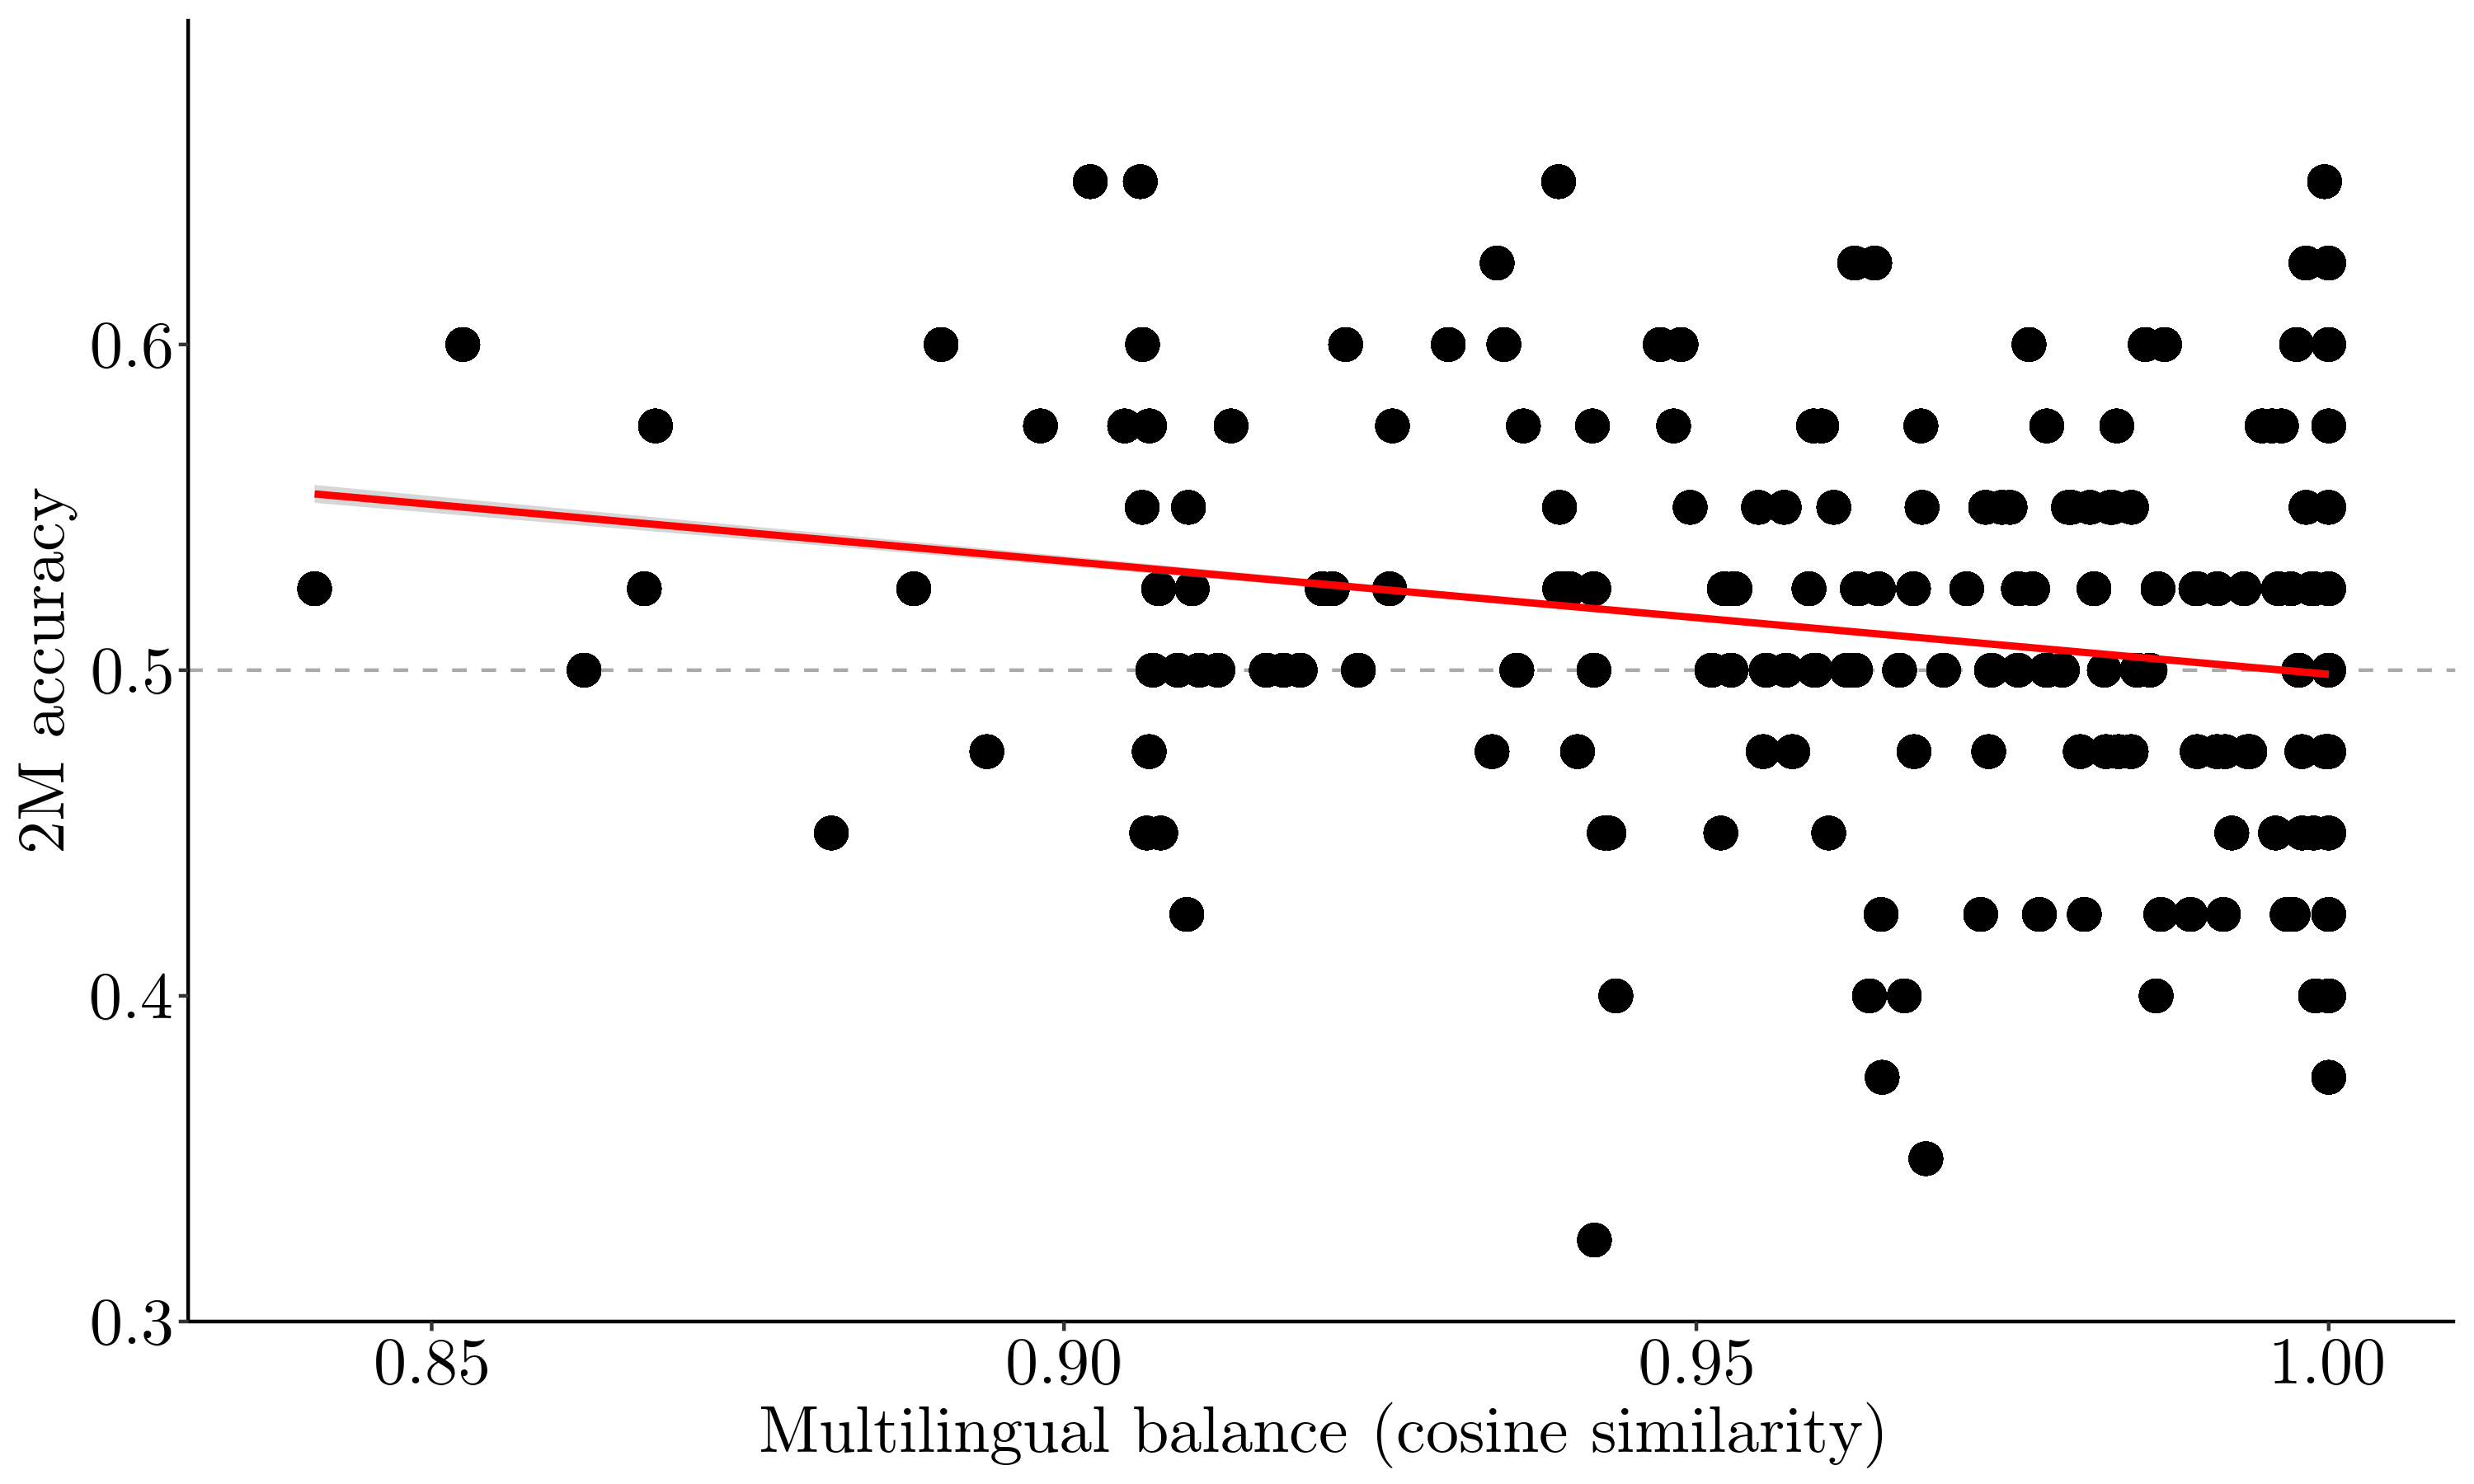
\includegraphics[width=0.99\textwidth]{Figures/exp3_2Mscore_cossim.png}
    \end{minipage}
    \begin{minipage}{0.49\linewidth}
        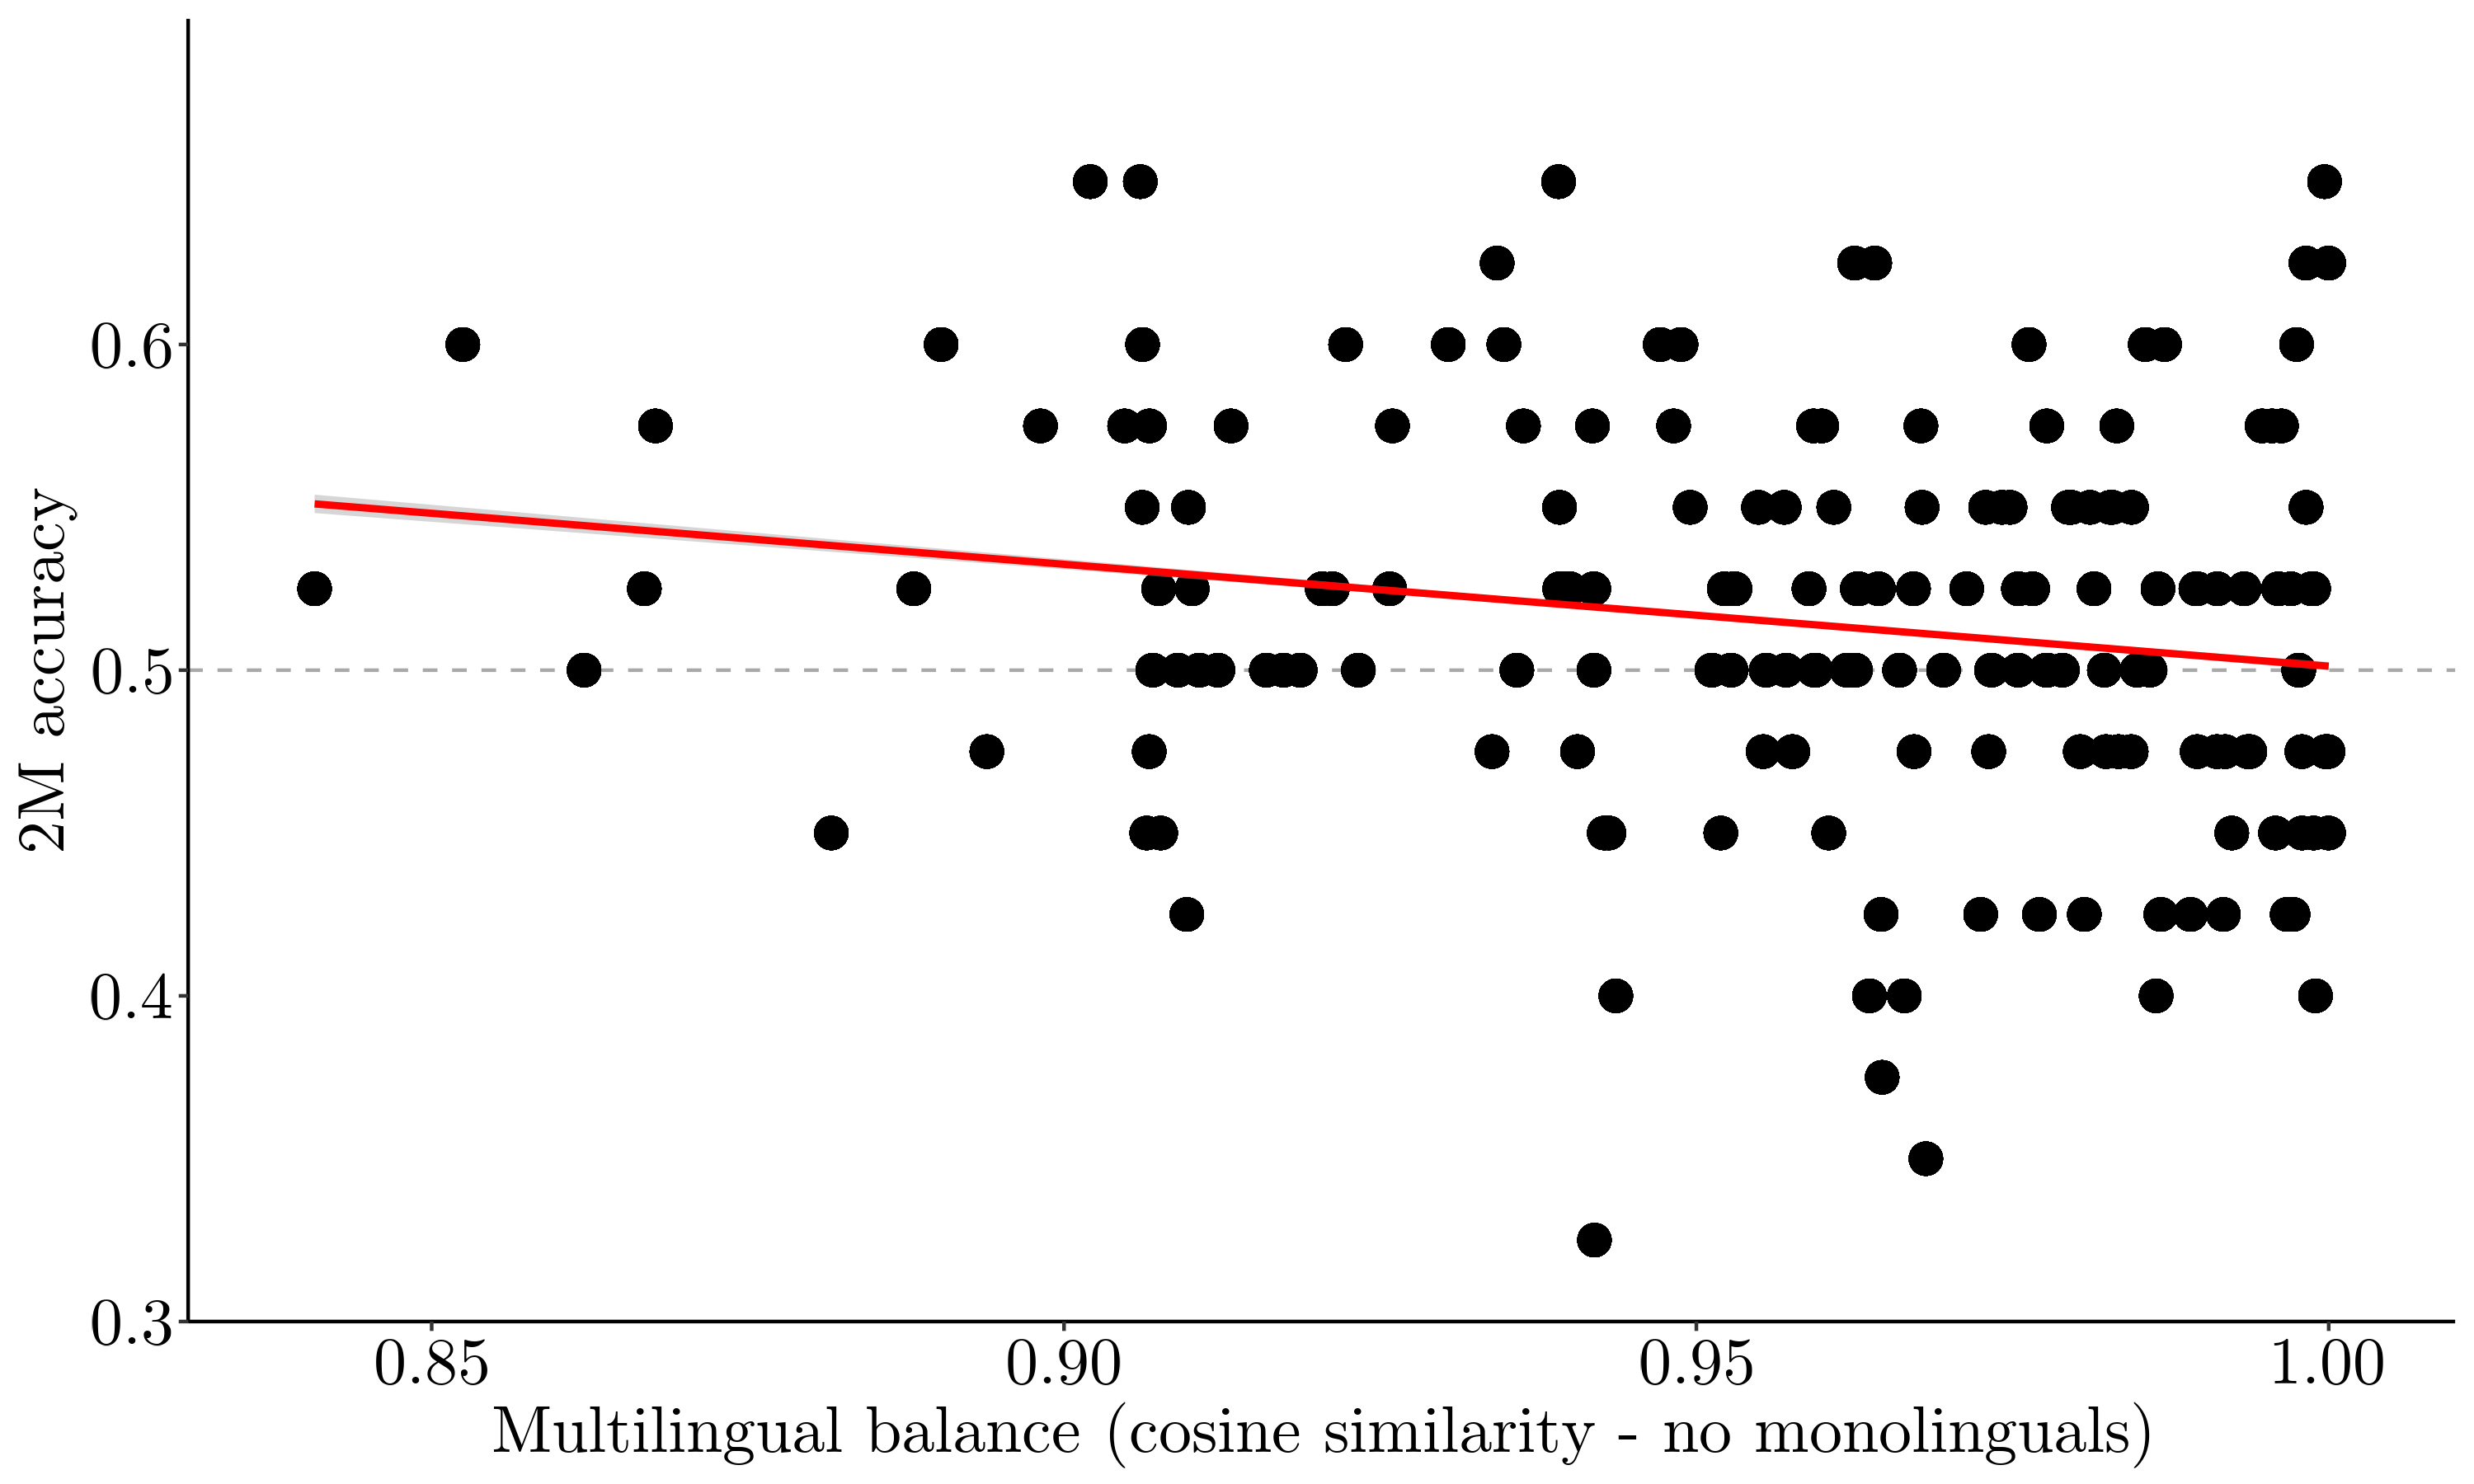
\includegraphics[width=0.99\textwidth]{Figures/exp3_2Mscore_cossim_nomonos.png}
    \end{minipage}
    \begin{minipage}{0.49\linewidth}
        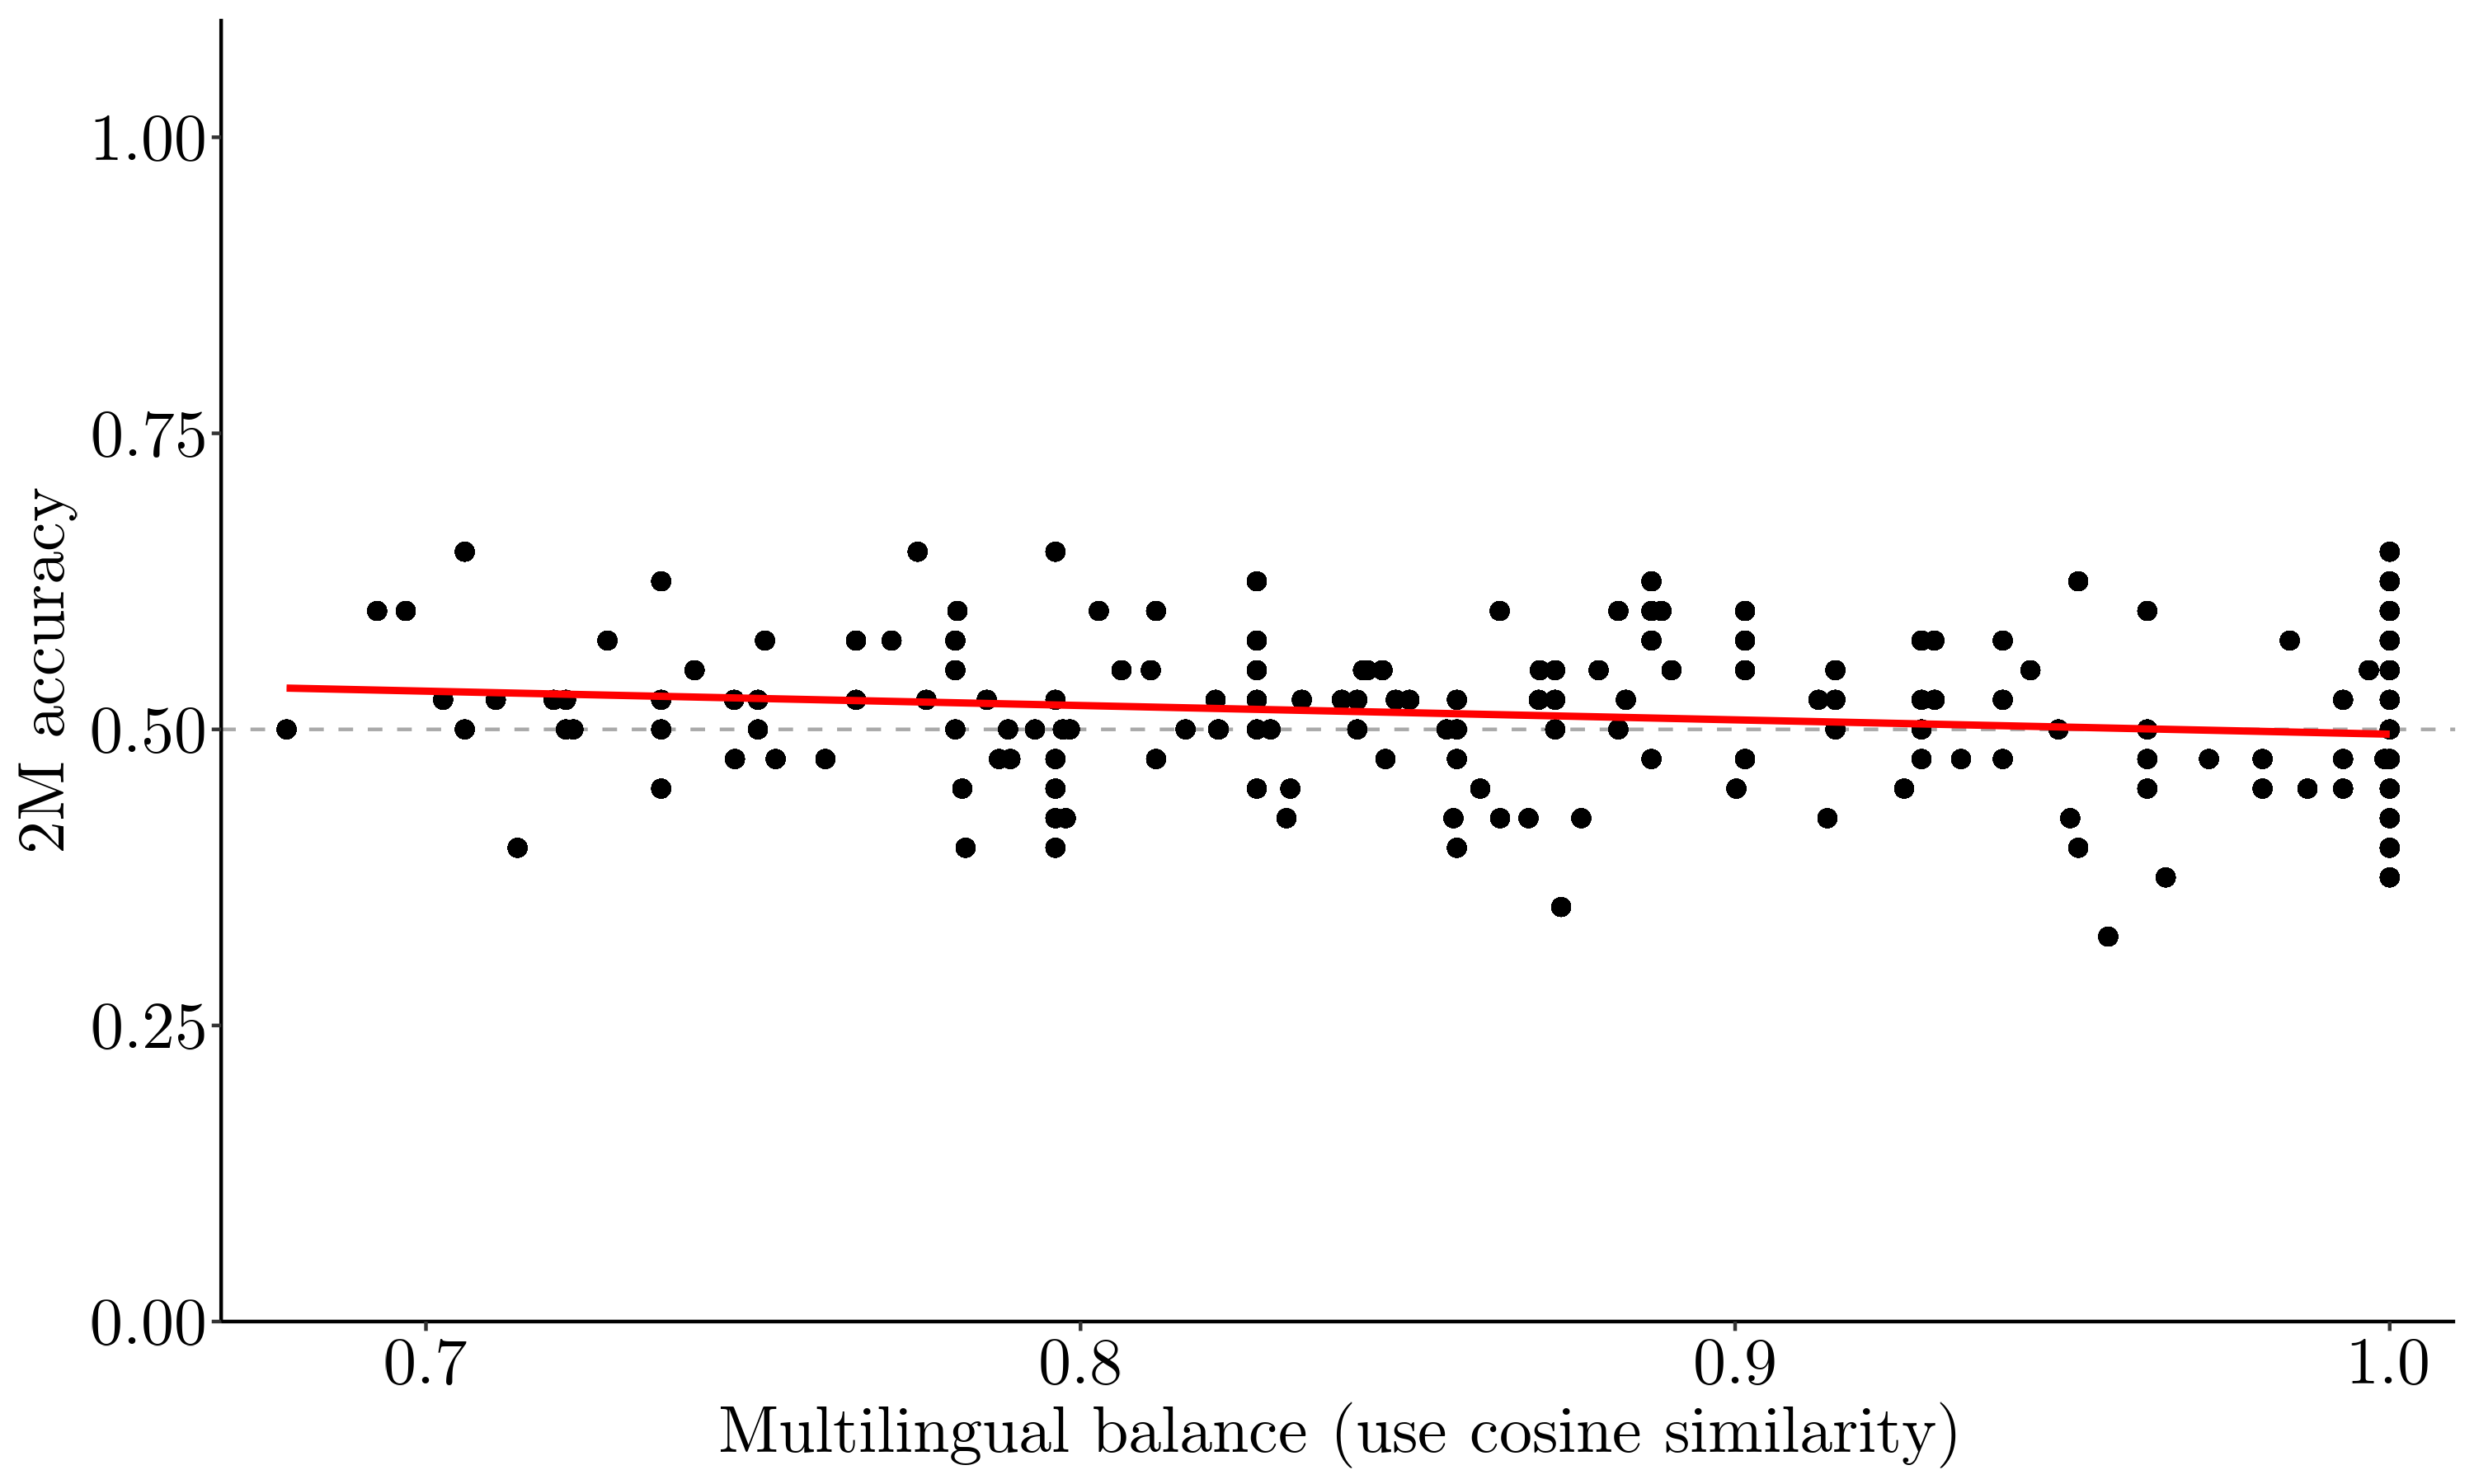
\includegraphics[width=0.99\textwidth]{Figures/exp3_2Mscore_use_cossim.png}
    \end{minipage}
    \begin{minipage}{0.49\linewidth}
        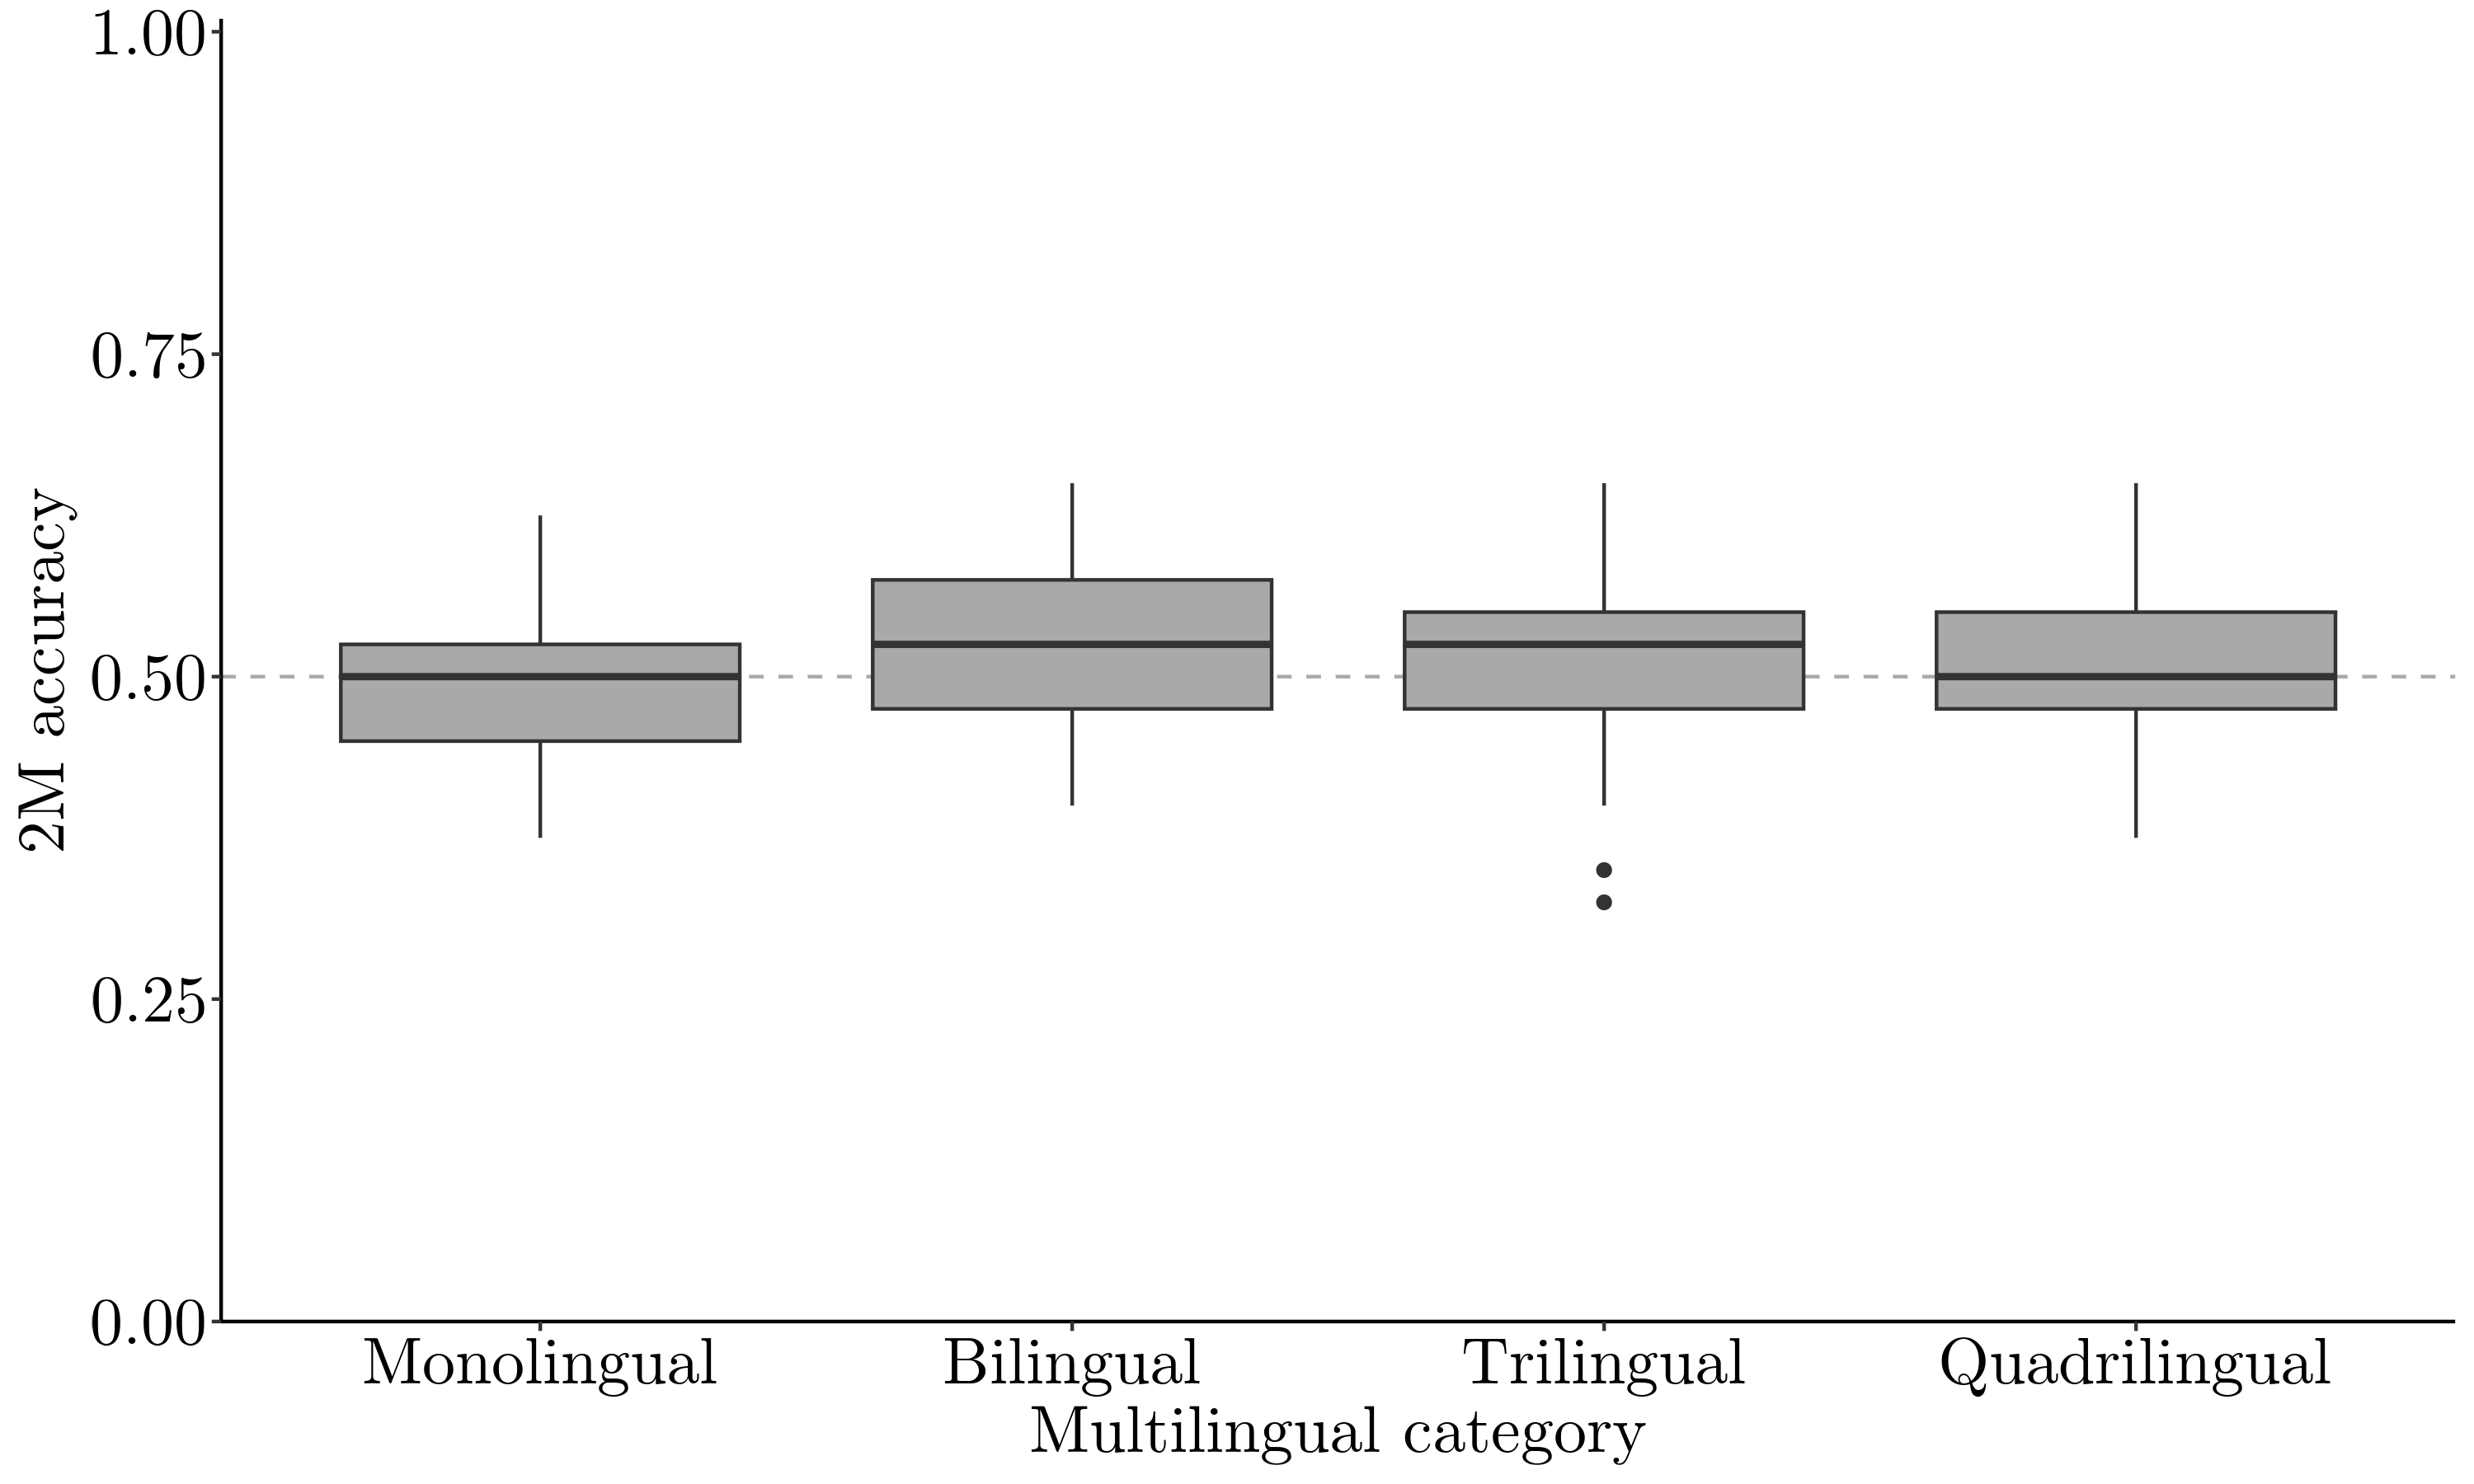
\includegraphics[width=0.99\textwidth]{Figures/exp3_2M_category.png}
    \end{minipage}
    \caption[]{\justifying Plots of the relationship between accuracy in the 2M condition and multilingual balance (cosine similarity, top left; without monolinguals, top right; use cosine similarity, bottom left) and multilingual category (bottom right). The dashed line at 0.5 indicates chance level.}
    \label{exp3_2Mcossim}
\end{figure}

\begin{table}[!htbp]
    \begin{center}
        \begin{tabular}{@{}lllll@{}}
            \toprule
            \multicolumn{5}{l}{\textbf{2M ``yes'' responses and accuracy}} \\ \midrule
            & \textbf{$\beta$} & \textbf{SE} & \textbf{z-value} & \textbf{p-value} \\ \midrule
            PC2 (L1 vs L2 use) & 0.18 & 0.06 & 3.10 & 0.002 \\ \midrule
            Multilingual experience & 0.15 & 0.06 & 2.58 & 0.0098 \\ \midrule
            L1-L2 difference & -0.15 & 0.06 & -2.74 & 0.006 \\ \midrule
            Mixed script & 0.24 & 0.11 & 2.14 & 0.03 \\ \midrule
            Cosine similarity & 0.11 & 0.06 & 1.99 & 0.047 \\ \midrule
            Cosine similarity$\ast$correct & -0.13 & 0.05 & -2.56 & 0.01 \\ \midrule
            Cosine similarity (no monolinguals)$\ast$correct & -0.11 & 0.05 & -2.02 & 0.04 \\ \midrule
            Use cosine similarity$\ast$correct & -0.11 & 0.05 & -2.24 & 0.03 \\ \midrule
            Bilinguals$\ast$correct & 0.34 & 0.16 & 2.08 & 0.04 \\ \bottomrule
        \end{tabular}
    \end{center}
    \caption{Summary of experiment 3 mixed modelling statistics of 2M ``yes'' responses and accuracy across conditions, for significant variables.}
    \label{exp3_2M_summary}
\end{table}
\break